\chapter{Thermal-Mechanical Design}  \label{thermal}

\section{Overview}
This chapter discusses the first of two major aspects of the LIFE design that are the focus of this thesis, the thermal-mechanical design. With previous instruments designed by the Atmospheric Research Group in ISAS, the thermal-mechanical design has played a smaller role. These instruments were not thermal imaging instruments and so had less stringent thermal requirements, and also had less power consumption which would lower any thermal effects. However, due to the complexity of these aspects with LIFE, it was determined that the thermal-mechanical design and analysis would play a major role and would require more research and simulations than previous instruments. The requirements that lead to the design are described in Section \ref{thermal_req_section}, which gives an overview of both the optical and electronic thermal ranges as well as the requirements for the mechanical design. The thermal environment is described in terms of how it relates to the thermal requirements and the simulations in Section \ref{thermal_env_ch3_sec}. The software used to develop both the design and perform the simulations is described in Section \ref{thermal_sim_sw_sec}, which also includes an overview of Finite Element Analysis. The description of the preliminary design and thermal simulations are found in Section \ref{prelim_design}, and finally the construction and testing of LIFE is described in Section \ref{preflight_const_analysis}.

\section{Requirements}\label{thermal_req_section}
Requirements always play a key role in any design, but may vary in how much they constrain the design process. Both the thermal requirements (set by the optical and electrical systems) and mechanical requirements (set by the CSA and CNES for the gondola) have had a large effect on the design. These requirements are described in detail in the following sections, before the design is described in detail, to provide background behind the design considerations. The optical system, being the most thermally sensitive and driving much of the LIFE design and thermal simulations, is described first. Following is the electrical system, which also has constraining requirements due to the high amount of heat dissipated as well as narrow operating temperature ranges. Finally, the mechanical constraints as set by CSA and CNES for the gondola flight are described.


\subsection{Optical Requirements}
The optical system, as with any thermal imagining instrument, must be carefully designed so that the thermal effect of the instrument from self-emission and temperature variations throughout flight due not have an effect on the data. Before describing the requirements for each component of the optical system, a Computer Assisted Design (CAD) model of the optical system is shown in Figure \ref{fig:optical_system_diagram} to illustrate all important optical system components. This will be described in greater detail in Section \ref{prelim_design}. A table summarizing the optical system requirements is presented at the end of this section, in Table \ref{optics_req_table}.

\begin{figure}[h]
\centering
  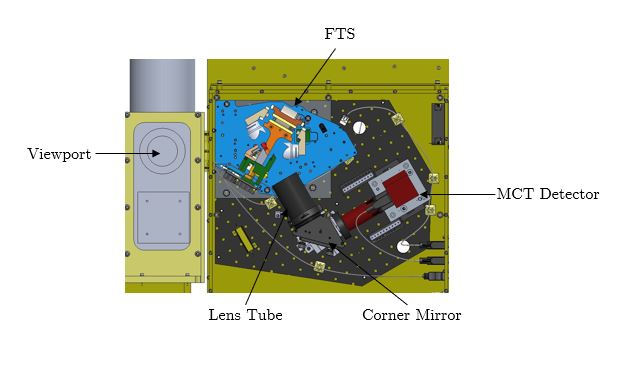
\includegraphics[width=\linewidth]{chap3_images/optical_system_diagram.JPG}
  \caption{CAD model of LIFE optical system.}
  \label{fig:optical_system_diagram}
\end{figure}

The optical system consists of the FTS, MCT detector, and imaging lens system between the FTS and detector. The first consideration is that the detector must be operated at 70K or lower as typical of MCT detectors. This requirement is already met by the pre-installed Stirling cooler that sits above the detector, so this requirement itself did not heavily influence the thermal design. However, something that still needs to be considered here is the removal of heat from this system. It must be ensured that the Stirling cooler is able to remove heat from the detector, either through conduction to the box walls or through sufficient radiation. Also, it must be considered that this removed heat will warm other components nearby, so must be designed for as well.

The lens array and FTS are the components that need to be most carefully thermally controlled. For this system, temperature requirements must be defined for environmental and mechanical reasons. Condensation in the lenses must be prevented during the ascent of the flight, where the instrument travels through the cold and humid troposphere. To provide a reasonable margin toa avoid the optics dropping to 0°C or below when condensation can form, a minimum temperature limit was set as 5°C. When operating in a warmer environment, such as the lab, thermal expansion of the lenses can be an issue, which may change optical properties and cause alignment problems. To avoid this, the maximum temperature requirement was set as 25°C. In addition to this temperature range requirement, the temperature drift must be considered as well. This is required to avoid issues with self-emission and removing the self-emission signal in the data analysis. As the time frame for multiple images of an instrument view (i.e. a blackbody or limb measurement) is on the order of minutes, the drift must be as small as possible over this range. A requirement is set at less than 0.1°C/min temperature drift over the lens and FTS components. 

The optical system mechanical requirements are to avoid any movement that could cause misalignment of the optics. It can be difficult to notice an issue with alignment as well as re-align the system, due to it being designed for non-visible light. The system must be as firmly built as possible to avoid any issues. There was originally also a mechanical requirement of removing vibrations from the system; small vibrations from the Stirling cooler were initially planned to be dampened or removed through some mechanical design. However, through discussions with ABB, it was determined that these vibrations would not have enough of a detrimental effect on the data to require a much more complex vibration dampening optics system design, and was removed from consideration.

\begin{table}[h]
\begin{center}
\begin{tabular}{ |c|c| }
 \hline
 \rowcolor{lightgray}
 System & Requirement\\
  \hline
  \hline
  MCT Detector & Temperature at 70K\\
 \hline
  MCT Detector & Dissipate heat to avoid overheating\\
 \hline
 FTS/Lenses & Temperature between 5°C - 25°C\\
 \hline
 FTS/Lenses & Temperature drift $<$ 0.1°/min\\
 \hline
 Mechanical & Minimize vibration\\
 \hline
\end{tabular}
\end{center}
\caption{Optical system requirements.}
 \label{optics_req_table}
\end{table}

\subsection{Electronics Requirements}\label{electronics_reqs}
The electrical components of LIFE have a wide variety of temperature ranges, which plays a large role in the design of the electronics box. There are a few particular components that have a narrow temperature range requirement, which must be placed accordingly in good locations and the temperature verified with simulations. The electronics are placed in a separate box from the optics; it is typical to place electronics in a separate box from the optical system, for both cleanliness and thermal reasons. The electronics in LIFE do not need to be as carefully controlled and kept as thermally steady as the optics, but it must be ensured that the temperature will not swing outside the required temperature range, especially during the ascent phase of flight through the tropopause. The most thermally sensitive components are the control board for the FTS system (BMXS Board), and the Ethernet interface boards (Pleora Boards) attached to the detector data acquisition (DAQ) boards. The thermal requirements for all major electronics in LIFE are detailed in Table \ref{therm_req_table}. 

\begin{table}[h]
\begin{center}
\begin{tabular}{ |c|c|c| }
 \hline
 \rowcolor{lightgray}
 Component & Minimum Temperature (°C) & Maximum Temperature (°C)\\
  \hline
  \hline
 BMXS Board  & 5 & 35 \\
 \hline
 CPU Stack (x2)  & -40 & 85 \\
 \hline
 DAQ Board (x2)  & -40 & 60 \\
 \hline
 DC-DC Converter & -40 & 85 \\
 \hline
 Ethernet Switch & -40 & 70 \\
 \hline
 Motor Driver & 0 & 60 \\
 \hline
 Pleora Board (x2)  & 0 & 40 \\
 \hline
 Temperature Controllers (x5) & -40 & 85 \\
 \hline
 VIPAC Power Supply & -40 & 95 \\
 \hline
\end{tabular}
\end{center}
\caption{Temperature limits of the major electrical system components.}
 \label{therm_req_table}
\end{table}

An important consideration in meeting these requirements is for the instrument to be able to dissipate enough heat in the warm scenario, without freezing in the cold scenario. Overall the total dissipation of the instrument is upwards of 500W, largely due to the two DAQ boards of 40W each. The instrument must be designed to move this heat away from these boards efficiently, and played a large role in the design.

\subsection{Mechanical Requirements}
The goal of the LIFE prototype was to fly on a high-altitude balloon gondola, and to do this the instrument had to meet mechanical requirements as outlined by CNES and the CSA. These requirements included volume, weight, bolt pattern, force and impact requirements. In addition to the gondola constraints, the instrument needed to be tested inside the ISAS Thermal Vacuum (TVAC) chamber, which provided further volume constraints.

\begin{figure}[h]
\centering
  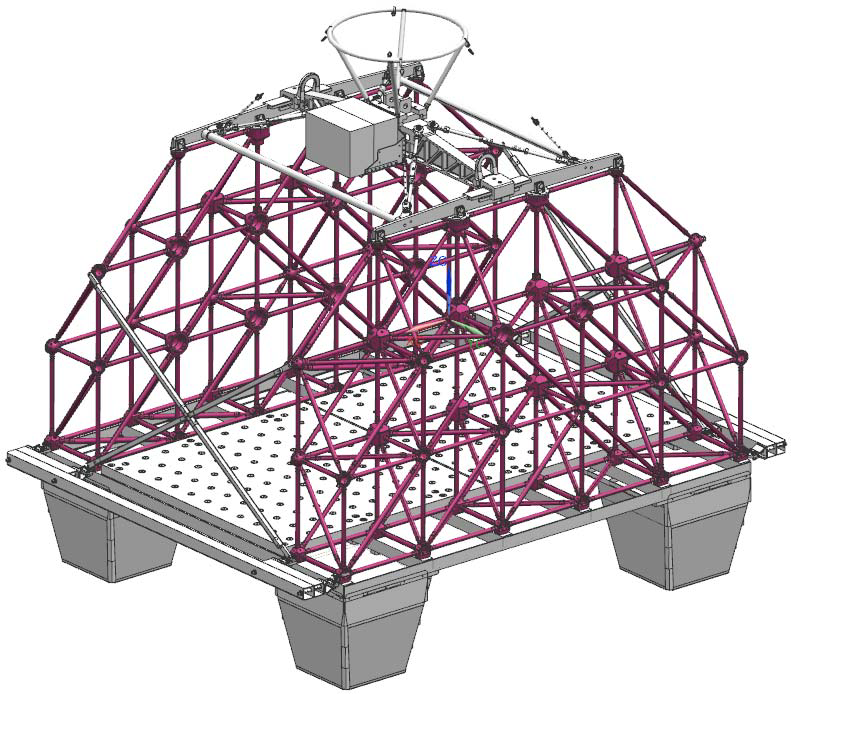
\includegraphics[width=0.7\linewidth]{chap3_images/Carmencita_empty.png}
  \caption{The CNES Carmencita gondola which carried LIFE for the test flight.}
  \label{fig:Carmencita_empty}
\end{figure}

CNES has multiple high-altitude gondola models of different sizes, and LIFE was designed to work with \textit{Carmencita}, the smallest model. A CAD model of Carmencita is shown in Figure \ref{fig:Carmencita_empty}~\citep{STRATOS_CARMENCITA_doc}. The design requirements that this gondola imposed upon the LIFE design were the volume, mass and bolt pattern constraints. As it is the smallest CNES gondola, and the flight was being shared with a few other smaller experiments, the CSA gave LIFE a maximum weight requirement of 100kg. In terms of size, the gondola is a modular design, forming 'boxes' with corner nodes that can be connected to other boxes. The size of one of these boxes is 342mm x 342mm, meaning that the total height of the gondola is 1.026m in the centre, sloping down to 342mm on the edge. No part of the instrument could protrude past this limit as a thermal blanket would be placed over top as a cover. LIFE was planned to be placed towards the centre of the gondola to maximize height allowance, but the sloping cover still needed to be taken into account, which could affect the LIFE maximum height depending on the width of the instrument. The honeycomb base plate panels that the instrument would attach to led to requirements for length and bolt pattern. The instrument base plate must match a 100mm x 100mm M6 pattern, and avoid protrusions used to attach the base plate to the structure. This gave a base plate length requirement of 950mm. The wall-to-wall length was slightly longer, at 1114mm~\citep{STRATOS_CARMENCITA_doc}. The TVAC chamber gives further volume requirements, with an internal size of 1006 x 813 x 794mm. A more detailed overview of the TVAC chamber is provided in Section \ref{TVAC_tests}. Both these dimensions and the Carmencita dimensions provided an overall size requirement of 950 x 813 x 794mm. 

LIFE had to meet numerous mechanical requirements as specified by the CSA. They provided an extensive Excel document which would calculate forces at each mechanical interface of the gondola to LIFE, as well as LIFE interfaces, to ensure it would survive a worst case force scenario. This was calculated at multiple angles from 0° to 315°, and calculated the maximum shear and tension forces based on the LIFE weight. A more detailed examination of these interfaces and forces calculated can be found in Section \ref{prelim_design} as the survival requirements depended on the detailed design, including mass and bolt pattern. However, one of the defining values for survival was the maximum force due to acceleration or shock. For the weight and size of the Carmencita gondola, this was given as 15g shock at ground impact. Other forces included rapid deceleration after parachute opening, at 8g. As LIFE was relatively heavy, it had to be ensured during design and through simulations that the connection between the instrument and the gondola, as well as connections between various parts of the instrument would be able to survive a maximum shock of this magnitude.

\section{Thermal Environment}\label{thermal_env_ch3_sec}
In addition to the stringent requirements given for the electrical and optical systems, these requirements need to be met in numerous environments, subject to a variety of conditions. The instrument must be designed by simulating different scenarios to ensure survival. This section discusses the main three environments the instrument will see, and the plan for simulations: the lab, the ascent phase of the flight, and the main float part of the flight. These environments formed the basis of the simulation temperatures and environments. 

\subsubsection{Lab Environment}
The instrument is most often operating in the lab environment. An air conditioning unit was installed in the lab to ensure that temperatures of both the instrument and the room would not increase substantially. The average temperature of the room was measured, so that the lab case for thermal simulations, known as the \textit{warm} case, could be determined as having an atmospheric temperature of 20°C, and a baseplate temperature of 15°C (based on the surface temperature of the table).

A difficult component of this environment to determine is convection. As described in Section \ref{heat_transfer}, it is difficult just to estimate a reasonable starting point for values such as the convection coefficient, which has a large impact on the resulting temperatures. Since this would have caused too much uncertainty in the model, convection is ignored for the lab environment simulations. Although this does make the simulations inaccurate, it provides a worst case scenario, as convection will only cool the instrument when the instrument is at higher temperatures than the room which is being cooled via air conditioning. Thus the baseline for the simulations was to set the baseplate temperature to 15°C and meet temperature requirements without the use of convection to cool. 

As a precaution for cooling, fans were planned to be installed in the instrument. The flow from these fans would cause forced conduction upon the electronics and cool everything quickly. This could theoretically be modelled via the SolidWorks Flow Analysis package, which would allow the simulations to be more accurate for the lab environment. However the package was deemed too difficult to use for this purpose, and unless there were serious temperature issues with the radiation and conduction based lab simulations, it would not be used.

\subsubsection{Flight Ascent Phase}
Ascent is the most rapidly changing environment, and also provides a wide array of unknowns, making it difficult to simulate properly. Ascent covers the phase from when the instrument is launched to when it reaches float altitude, covering over 30km. Both temperature and pressure change rapidly in this region, and for the LIFE flight from Timmins a pressure variation from 1000hPa to 3hPa and a temperature range from 10°C to -70°C can be seen as a worst case scenario. This minimum temperature can occur for as long as 60 minutes~\citep{STRATOS_CARMENCITA_doc}. These changes lead to difficulty in the simulation of convection, which depends on a number of variables, including temperature and pressure.

Due to the uncertainty in most simulation variables, this phase was chosen not to be modelled before flight. From previous instruments, it was found that although the temperature drop through the ascent has a noticeable effect, it is not in this region long enough to freeze and damage electronics. Further, there are no papers or materials on the change in convection in this pressure or temperature range; studies are typically done in warm environments at higher pressures, for the purpose of studying mechanical systems. It was decided that the instrument would be designed to withstand the worst case cold scenario at float altitude, and post-flight a simulation would be created based on the measured temperature through ascent, to inform future instruments and missions.

\subsubsection{Flight Float Phase}
At float altitude, the environment is fairly well defined and stable. Thus the instrument can be designed to survive and operate here with reasonable certainty in simulations. Although the measurements of the LIFE instrument do not depend on the time of day or night, it is chosen to fly at night to further define the thermal environment. It removes the possibility of seeing the sun, which presents issues such as solar heating and radiation, both of which are not well defined and are based on the viewing geometry of the instrument with respect to the sun, as well as what parts are shaded. In the night environment, the only external thermal impact on the instrument is due to conduction between the instrument baseplate and the gondola. As measured during the CATS flight and discussed in Section \ref{balloon_env}, the coldest the gondola will get is -40°C. This was used as the worst case cold scenario for the initial simulations. For the majority of the flight, the baseplate will sit between -20°C and -30°C, so the most common scenario, or the middle simulation case, was a baseplate at -30°C. In total, there are three initial simulation cases: 20°C (lab, warm case), -30°C (float, base case), -40°C (float, coldest case, following ascent). 

During flight, due to the unavailability of a landing site, the landing was delayed until the afternoon, well after the sun had risen. So even though the sun case was not considered in the design, it played a role in the resulting thermal data and should be described here. If a flight is planned to go past sunrise, sun shields are installed on the gondola to provide shade for the instruments to reduce solar heating. However since the daylight part of the flight was not planned, the sun had a significant affect on instrument temperatures. Solar heating at this altitude, due to the lack of atmosphere, can have a very strong impact on the temperature of an instrument if the absorptivity of a material is high. An example given from the CSA is a black anodized aluminum material, with an absorptivity $\alpha$ of 0.67, will reach a surface temperature of 117°C in direct sunlight of 1400 $W/m^2$ solar flux at float ambient temperature~\citep{STRATOS_CARMENCITA_doc}. Radiation will also be effected, as the object seen by the surface is at a very high temperature, as opposed to the cold atmosphere or deep space. The effects on LIFE of the part of the flight after sunrise is described and analyzed in Chapter \ref{postflight}.

Finally, the float component of the flight is good to simulate thermally as the simulations can be verified in the lab through the use of a Thermal Vacuum chamber (TVAC). With a vacuum environment and a cold plate that can reach -40°C through the use of liquid nitrogen, it can provide a good test of the actual flight float environment. Comparing results of the simulation to the actual results of a TVAC also helps to determine the answers to a number of questions, such as basic survivability, but also unknowns such as heat transfer coefficients across gaps. A more detailed discussion on the LIFE TVAC tests can be found in Section \ref{TVAC_tests}.

\section{Thermal-Mechanical Design \& Simulation Software}\label{thermal_sim_sw_sec}
With previous instruments, the thermal requirements were not overly stringent, and the thermal design could be estimated with simple calculations and knowledge of previous missions. With the LIFE requirements it was determined that this would not provide enough accuracy for flight, and a full thermal analysis of the instrument was needed. A thermal model was to be created, based on the instrument mechanical model. It would analyze the thermal performance in different flight and lab environments, and determine the necessary methods required to keep the instrument above freezing as well as to dissipate enough heat. Both mechanical and thermal designs were iterated many times before coming to a final design solution. The software used to perform the analysis and design is described here. This section also explains the basis behind many design analyses, Finite Element Analysis, and relates this to how this is used in LIFE thermal simulations.

\subsection{Computer Assisted Design Software}
There are a wide variety of Computer Assisted Design (CAD) software available, and they are all used widely in industry. A large subset of these can also perform thermal analyses within the program. Research was done into different software to determine which would best suit the needs of the LIFE simulations. Two final options were found: Siemens NX and SolidWorks, both the most popular options in industry.

Siemens NX, developed by Siemens AG, is a CAD software heavily used throughout industry for advanced modelling of large designs, and particularly thermal simulations. It was recommended for the LIFE project by Honeywell Aerospace, who used the software to develop the thermal models of the CATS and ALI (Aerosol Limb Imager) instruments that the ISAS group has co-developed. NX thermal modelling software is widely considered the most advanced in the industry, particularly in aerospace design. However, downsides to NX are a very steep learning curve and price. Regardless, the thermal simulation software would likely be the best to suit the needs of LIFE.

SolidWorks, developed by Dassault Systems, is likely the most popular CAD software available. It is designed more for modelling of smaller designs and parts rather than large assemblies, and has overall less functionality. While this is a downside, it also has an easier learning curve and academic licenses are easily available, which cuts down on cost. Due to its popularity, there is a large amount of community support through forums and online tutorials on both its basic functionality and simulation abilities. Further, the early initial CAD model of LIFE had already been designed in SolidWorks; using the thermal analysis functionality of the program would be much simpler, not having to rely on exporting to another software. The thermal simulation suite, which comes built-in with an academic license, does not have the same depth as NX. This will lead to less accurate simulations. SolidWorks does have an electronics thermal modelling package as an add-on, which could be beneficial to the design. However the complexity of the package was larger than necessary, and is meant more for board-level electronics designs. As such it was not considered in the final decision. Overall however, due in large part to the much cheaper cost and prior experience in the software, SolidWorks was eventually chosen to be used for the simulations and to develop the CAD model further. 

The mechanical model for LIFE, as is described in depth in Section \ref{prelim_design}, is designed entirely using SolidWorks. The thermal design is discussed in tandem with the evolution of the mechanical design, as they are heavily connected. Simulations were done with the aforementioned built in thermal software, and some structural simulations as well. The basis behind all SolidWorks simulations is an analysis technique known as Finite Element Analysis.

\subsection{Finite Element Analysis} \label{FEA}
Finite Element Analysis (FEA), also sometimes referred to as the Finite Element Method (FEM), is one of the most important numerical analysis tools available for engineering design. It allows any arbitrary surface or shape in any number of dimensions to be analysed and simulated numerically. Almost all CAD software simulations utilize FEA at its basis. FEA, overall, is a process of converting any shape along with its sources and restraints that can be represented by differential equations to a system of matrices that can be solved to give an approximate solution~\citep{FEA_SW}.

The basis of FEA is to replace any complex shape or model with simple shapes, that when summed together create the original shape. These simple shapes, which are dependent on the simulation but most often some type of triangle, are known as finite elements. These can be compared to the original model in the same way that finite elements of a sum can be compared to infinitesimal differential elements of integral equations. The elements can be altered in numerous ways, including shape and size, to work best for each simulation~\citep{FEA_SW}. The array of elements when it is applied to a part is known as a mesh. An example of a shape being converted into both a coarse mesh and fine mesh with slightly different shapes is shown in Figure \ref{FEA_mesh_example}.

\begin{figure}
    \centering
    \begin{subfigure}[h]{0.6\textwidth}
        \centering
        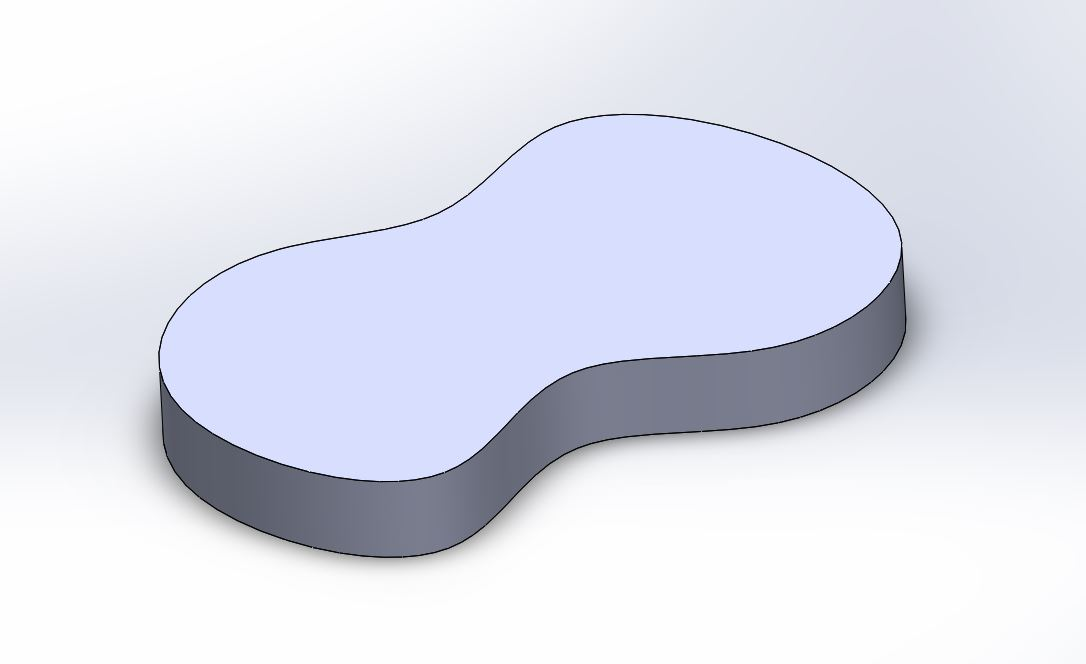
\includegraphics[width=\textwidth]{chap3_images/mesh_test_part_no_mesh.JPG}
        \caption{Example SolidWorks part, before elements applied.}
        \label{fig:FEA_mesh_before}
    \end{subfigure}
    \begin{subfigure}[h]{0.6\textwidth}
        \centering
        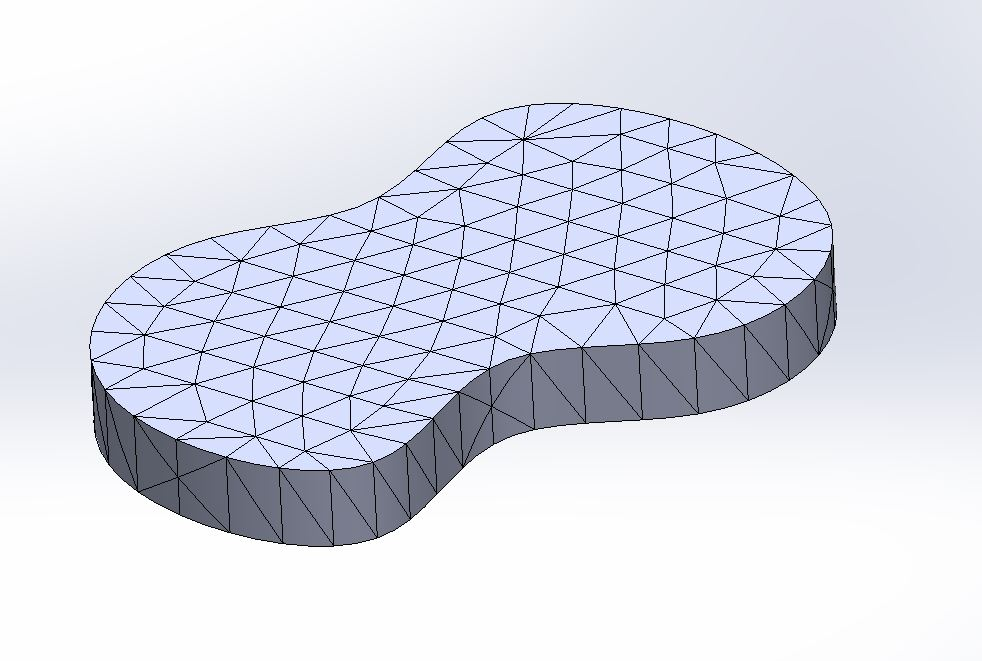
\includegraphics[width=\textwidth]{chap3_images/mesh_test_part_coarse_mesh.JPG}
        \caption{Example SolidWorks part, with coarse, regular elements.}
        \label{fig:FEA_mesh_coarse}
    \end{subfigure}
    \begin{subfigure}[h]{0.6\textwidth}
        \centering
        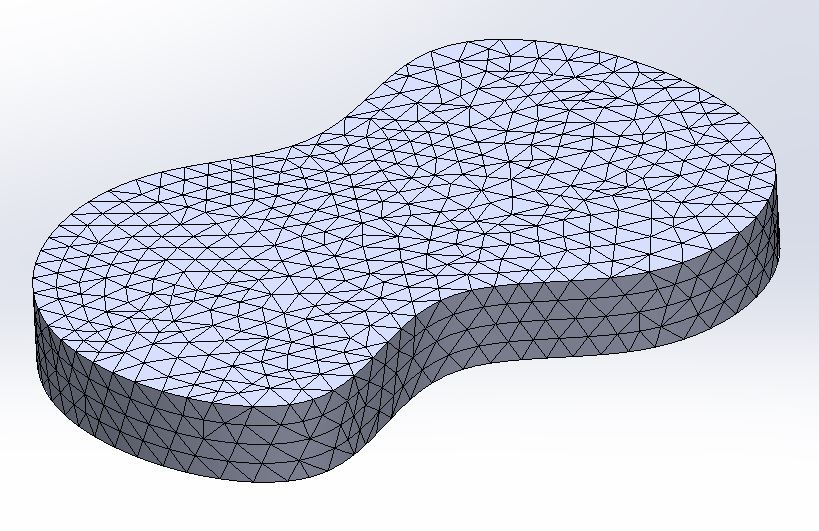
\includegraphics[width=\textwidth]{chap3_images/mesh_test_part_fine_mesh.JPG}
        \caption{Example SolidWorks part, with fine, curved elements.}
        \label{fig:FEA_mesh_fine}
    \end{subfigure}
    \caption{A shape being converted to finite elements, or a mesh.}
    \label{FEA_mesh_example}
\end{figure}

The volume of this part could now be easily calculated. The choice of element shape must be considered when creating the mesh; Computationally, the linear triangle, as shown in Figure \ref{fig:FEA_mesh_coarse}, is easiest to solve using a simple area equation for a linear triangle. All that is needed is the vertex components for all triangles to be able to calculate the area or volume. A quadratic triangle with curved sides, as shown in Figure \ref{fig:FEA_mesh_fine}, is better at approximating curved shapes, however more advanced numerical integration is needed to solve for the area or volume of a quadratic triangle~\citep{FEA_SW}. It is a trade-off that must be considered between error and simulation solve time, but often there is no choice, especially working with a lot of curved components, that the latter and more computationally expensive option must be used. By default, SolidWorks uses quadratic triangles, but use higher polynomial shapes if necessary. Tetrahedral elements are always used for volume components in SolidWorks. 

The evaluation of an FEA problem relies heavily on the mesh, and particularly its vertices. The mesh generates two arrays: The first is a list of all vertices, with their spacial coordinates, and is known as the nodal set. The second is known as the connectivity list and describes each vertex along with the vertices that it is connected to. This list is critical to solving analyses and simulations, as these inform the matrices and equations used for the solution~\citep{FEA_SW}. For each vertex in the mesh, there is one simultaneous equation that describes every equation or variable that may impact the final values at that node. 

For whatever type of simulation is being done, the general equilibrium matrix will always be the same. It is simplest to show this with the well-known spring system, following the example in the textbook \textit{Finite Element Analysis Concepts via SolidWorks}. For the problem of a single spring that is generalized so that either side can be restrained or loaded with force, the equilibrium equations can be shown as the matrix form in Equation \ref{spring_FEA_matrix}.

\begin{equation} \label{spring_FEA_matrix}
\begingroup
    k
    \begin{bmatrix}
        1 & -1 \\
        -1 & 1
    \end{bmatrix}
    \begin{Bmatrix}
        u_1 \\
        u_2 \\
    \end{Bmatrix}
    =
    \begin{Bmatrix}
        f_1 \\
        f_2 \\
    \end{Bmatrix}
\endgroup
\end{equation}

Here $k$ is the stiffness, $u$ is the displacement, $f$ is the force, and the subscripts correspond to each side of the spring. This can be used to represent a node of the matrix. However, in this form the equation cannot be solved; there is only information about this one node. Information must be given as an initial condition, i.e. displacement, and boundary conditions, i.e. force. If the initial condition is given as $u_{given}$ and the force on one end of the spring is given as $F$, then Equation \ref{spring_FEA_matrix} can be written as Equation \ref{spring_FEA_matrix_solvable}.

\begin{equation} \label{spring_FEA_matrix_solvable}
\begingroup
    k
    \begin{bmatrix}
        1 & -1 \\
        -1 & 1
    \end{bmatrix}
    \begin{Bmatrix}
        u_{given} \\
        u_2 \\
    \end{Bmatrix}
    =
    \begin{Bmatrix}
        F \\
        f_2 \\
    \end{Bmatrix}
\endgroup
\end{equation}

This leaves the displacement of the other end of the spring and the reactionary force to be solved for. The two given values would be input into SolidWorks, say as the force on a plate and its initial displacement, and it would calculate how far the next node would move based on its force and displacement from the initial node. This is calculated for all nodes in the mesh. This equation becomes much more complex as more nodes are added and as the shape of the elements becomes more complex, leading to more inputs on each node from other nodes. The general equation for the mechanical displacement problem is given in Equation \ref{gen_FEA_matrix}.

\begin{equation} \label{gen_FEA_matrix}
\begingroup \boldmath
    \begin{bmatrix}
        K_{uu} & K_{ug} \\
        K_{gu} & K_{gg}
    \end{bmatrix}
    \begin{Bmatrix}
        \Delta_u \\
        \Delta_g \\
    \end{Bmatrix}
    =
    \begin{Bmatrix}
        F_g \\
        F_u \\
    \end{Bmatrix}
\endgroup
\end{equation}

Here, $\bm{\Delta_u}$ are the unknown nodal displacements, $\bm{\Delta_g}$ are the given boundary values of other displacements, such as a restraint on the edge boundary of a part. For a known part, all values of the $\bm{K}$ matrices are known. The applied loads to the nodes is represented by $\bm{F_g}$, with $\bm{F_u}$ as the unknown reaction forces from other nodes and their boundary conditions. As there are only two unknowns remaining, this general matrix can be solved. 

Structural and thermal analysis have a number of analogous terms, making it simple to use Equation \ref{gen_FEA_matrix} in thermal simulations be changing a few variables. A table showing the conversion from structural analysis to thermal analysis is shown in Table \ref{mech_to_thermal_properties}~\citep{FEA_SW}.

\begin{table}[h]
\begin{center}
\begin{tabular}{ |c|c|c| }
 \hline
 \rowcolor{lightgray}
 Equation Component & Thermal Variable  & Mechanical Variable\\
  \hline
  Unknown & Temperature, T [K] & Displacement, u [m]\\
  \hline
 Gradient & Temperature gradient, $\Delta T$ [K/m] & Strain, $\epsilon$ [m/m]\\
 \hline
 Flux & Heat flux, q [W/m\textsuperscript{2}] & Stress, $\sigma$ [N/m\textsuperscript{2}]\\
 \hline
 Source & Heat source, Q [W] & Force, g [N]\\
 \hline
 Indirect restraint & Convection & Elastic Support \\
 \hline
 Restraint & Set temperature, T [K] & Set displacement, u [m]\\
 \hline
 Reaction & Heat flow, H or Q [W] & Force, F [N]\\
 \hline
 Material Property & Thermal conductivity, k [W/mK] & Stiffness, k [N/m\textsuperscript{2}]\\
 \hline
 Law & Fourier's Law & Hooke's Law\\
 \hline
\end{tabular}
\end{center}
\caption{Equivalents between thermal and mechanical simulations.}
 \label{mech_to_thermal_properties}
\end{table}

Thermal simulations with FEA all have a single equation governing each node, as in mechanical simulations. All above components of the equation are considered within this equation. This includes heat flux due to heat power, radiation, and conduction, the convection restraint, restraints on specified temperatures (for example, the base plate must be -40°C as a worst-case scenario), the reactions are the resultant heat flow that is necessary to maintain the specified temperatures, and the final unknown is the temperature. All other conditions add source terms, such as the dissipated heat power of electrical components~\citep{FEA_SW}.

For thermal equilibrium, the resulting matrix equations have a general form as shown in Equation \ref{gen_T_matrix}.

\begin{equation} \label{gen_T_matrix}
\begingroup \boldmath
    \begin{bmatrix}
        K_{uu} & K_{ug} \\
        K_{gu} & K_{gg}
    \end{bmatrix}
    \begin{bmatrix}
        T_u \\
        T_g \\
    \end{bmatrix}
    =
    \begin{bmatrix}
        F_g \\
        F_u \\
    \end{bmatrix}
\endgroup
\end{equation}

where $\bm{T_f}$ represents the restrained vertex temperatures and $\bm{F_g}$ represents the thermal heat power (heat flow) of the vertex. The $\bm{K}$ values represent the thermal conductivity matrix for each node, where if the material is assumed isotropic is unit matrix. $\bm{F_u}$ is unknown and represents the total heat flow in or out of a node that is necessary to maintain the given temperatures $\bm{T_g}$. $\bm{F_g}$ is calculated with heat flux, which is where conduction and radiation equations are used in the solution. For thermal conductive heat flux, Fourier's Law is used, from Equation \ref{FC_law}. Heat flux incident on the body and radiation from the body is from Equation \ref{SB_surroundings}. $\bm{F_u}$ is thus calculated from adding the conductive flux from Equation \ref{FC_law} the radiation flux from Equation \ref{SB_surroundings}, and the flux resulting from $\bm{F_g}$. This allows to complete the goal of the equations which is to solve for $\bm{T_u}$~\citep{FEA_SW}~\citep{FEA_Procedures}. An example solution equation for the temperature at a node would look like Equation \ref{TA_solution_eq}.

\begin{equation}\label{TA_solution_eq}
    \bm{T_u = K_{uu}^{-1}(F_g-K_{ug}T_g)}
\end{equation}

In a simple example part in a vacuum environment, $\bm{T_g}$ would be an array of constants as chosen for the simulation, k would be a constant material conductivity if the material was isotropic, and $\bm{F_g}$ would the conductive heat flow plus the radiative heat flow. 

The size of the set of equations that is in general given by Equation \ref{gen_FEA_matrix} is the number of nodes. Thus, for an example of 100,000 nodes, there are 100,000 equations, and 100,000 temperatures calculated. Putting all these nodes together in the CAD model gives a solved thermal model necessary for thermal analysis.  The model can be evaluated for both lab and flight conditions by including or neglecting convection respectively, and by specifying relevant boundary conditions. 

\section{LIFE Thermal-Mechanical Design Process}\label{prelim_design}
The preliminary design for LIFE was completed using SolidWorks, through a series of iterations of different components of the instrument. In all, the instrument can be split into four major parts: The blackbody system, the box containing the optical system, the main electronics box which contains electrical parts for the FTS and detector as well as the computers, and finally a smaller electronics box that contains the electronics used to control the blackbodies. To give an overview for how these parts are connected before going into detail of the design process for each, a block diagram of LIFE is provided in Figure \ref{fig:LIFE_block_diagram}.

\begin{figure}
    \centering
    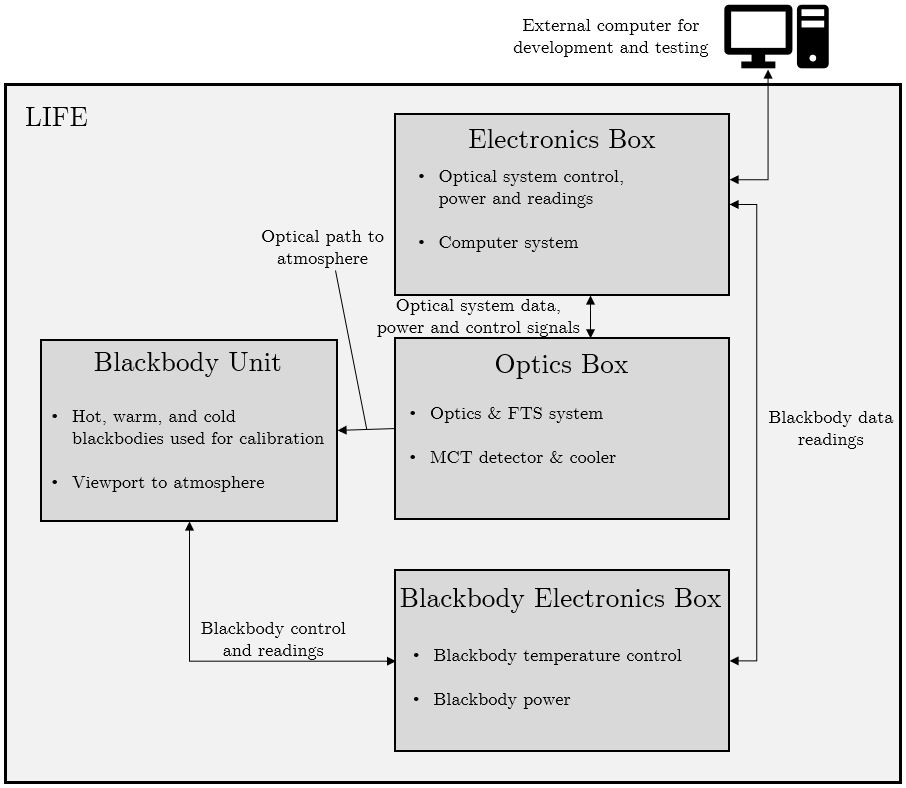
\includegraphics[width=\linewidth]{chap3_images/LIFE_block_diagram.JPG}
    \caption{Block diagram of the LIFE instrument.}
    \label{fig:LIFE_block_diagram}
\end{figure}

Although there are fluctuations through the design process, it is helpful to give an overview of the purpose of each component. The blackbody assembly houses the three blackbodies that the instrument images during calibration and testing, which was procured from ABB. The instrument also views the atmosphere through this unit, through a side viewport. This system is described in greater detail in Section \ref{blackbody_assem_sec}. The optics box houses all the core components of the imaging system of the instrument: The lens array, the FTS, and the detector. These are all mounted to an optical breadboard plate, which is mounted to the side of the box interior for FOV purposes. The optical path goes out of the Optics Box and into the blackbody unit, where it is reflected into the atmosphere. The Electronics Box houses the parts necessary for operation of all components of the instrument, except for the blackbodies. This includes the data acquisition boards for the detector, the control board for the FTS, the computer system, multiple power supplies, and its own heaters and temperature controllers. As such, there are critical connections between the optics and electronics box that carry the sensitive data signals from the detector as well as control signals to and from the FTS. This box also interfaces with an external computer, which can be used if necessary to control and read data from the instrument during the development and testing phase, as well as troubleshooting. Finally, the Blackbody Electronics Box houses the electronics necessary for operation of the blackbodies, such as the temperature controllers and power supply. In early iterations, the electronics in this box were part of the main electronics box, until the size grew too large for the volume requirements of the CNES gondola. It sends this data to the main computer in the electronics box.

The LIFE instrument went through a large number of design iterations before reaching the final design that was constructed and launched. Each subsection below, with the exception of the Blackbody Assembly (as it did not play a role in the design iterations), discusses a version of the design. This includes a detailed description of the optics and electronics boxes, which each went through a number of their own versions, and the thermal analysis done for each. The thermal analysis often formed the basis for a new version of the design. The final section goes into further detail about the final version and the detailed thermal analysis that was done to prepare it for TVAC tests and the flight.

\subsection{LIFE Preliminary Design: Blackbody Assembly}\label{blackbody_assem_sec}
The blackbody assembly, unlike the rest of the design, was not designed in-house. It was procured separately from ABB for use in the LIFE instrument, to save the cost of designing and building or purchasing a new blackbody system. However, it still required work to characterize the blackbodies to ensure proper operation and to ensure that they would work properly with LIFE. They also play an important part in the overall LIFE design, so they will be described here.

The blackbody assembly has six blackbody surfaces that can be imaged. The original purpose of the instrument required two identical systems, so there are two entrance viewports, three pairs of blackbodies, and two exit viewports towards the atmosphere. LIFE only requires one system, so the other was used only for lab verification testing. Focusing now on one part of the system, there are three surfaces that can be imaged. The cold blackbody surface is connected to a thermoelectric cooler. The minimum temperature of this cooler is unknown, but is rated to go well below 0°C. However, in a lab environment, the surface temperature dropping below zero would lead to frost buildup on the surface, causing changes in the emissivity. With changes in the emissivity, the temperatures would no longer be measured properly, and in addition the frost buildup could cause dust and other materials to build up on the surface, rendering it less accurate. Thus the lowest temperature this blackbody was set at was 5°C, and was set to 10°C for the majority of our testing. Another external blackbody, from the ACE instrument, was procured from ABB for the purposes of looking at a temperature well below freezing, in a TVAC environment. This is described in greater detail in Section \ref{non-linearity_sec}. 

The other two surfaces can theoretically be used interchangeably as the hot and warm blackbody surfaces, however it was discovered that the power of the heater inside one surface is much larger than the other, so to ensure enough power to reliably keep the temperatures steady, the former was chosen as the hot blackbody surface. During tests, the blackbody surfaces were interchanged, and in a cold environment there is not enough power to keep the temperature steady for the hot blackbody with the lower power heater. No maximum temperature was given for these surfaces, but were used in their original configuration as high as 225°C. In the LIFE configuration, most often the hot blackbody was set at 60°C and the warm blackbody was set at 30°C. A schematic of the blackbody system is shown in Figure \ref{fig:bb_schematic}, and a CAD model of the system is shown in Figure \ref{fig:CAD_Blackbodies}.

\begin{figure}
    \centering
    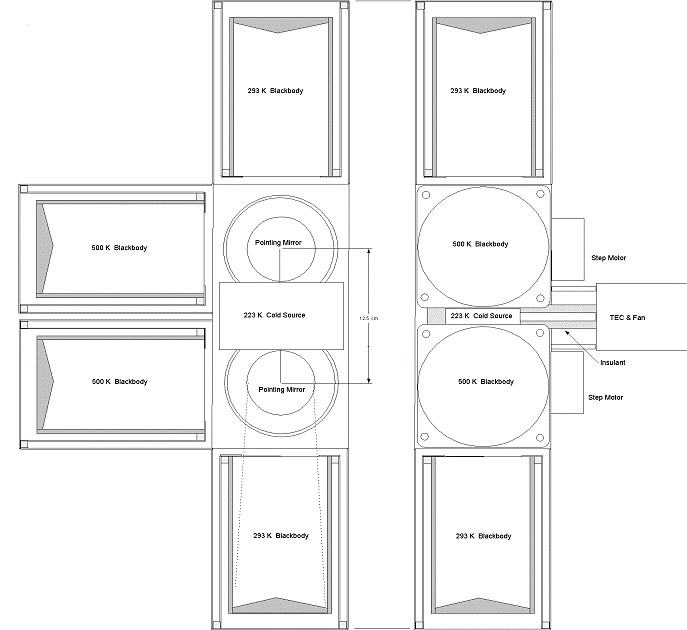
\includegraphics[width=\linewidth]{chap3_images/Blackbody_schematic.png}
    \caption{Schematic of the LIFE blackbody system.}
    \label{fig:bb_schematic}
\end{figure}

\begin{figure}
    \centering
    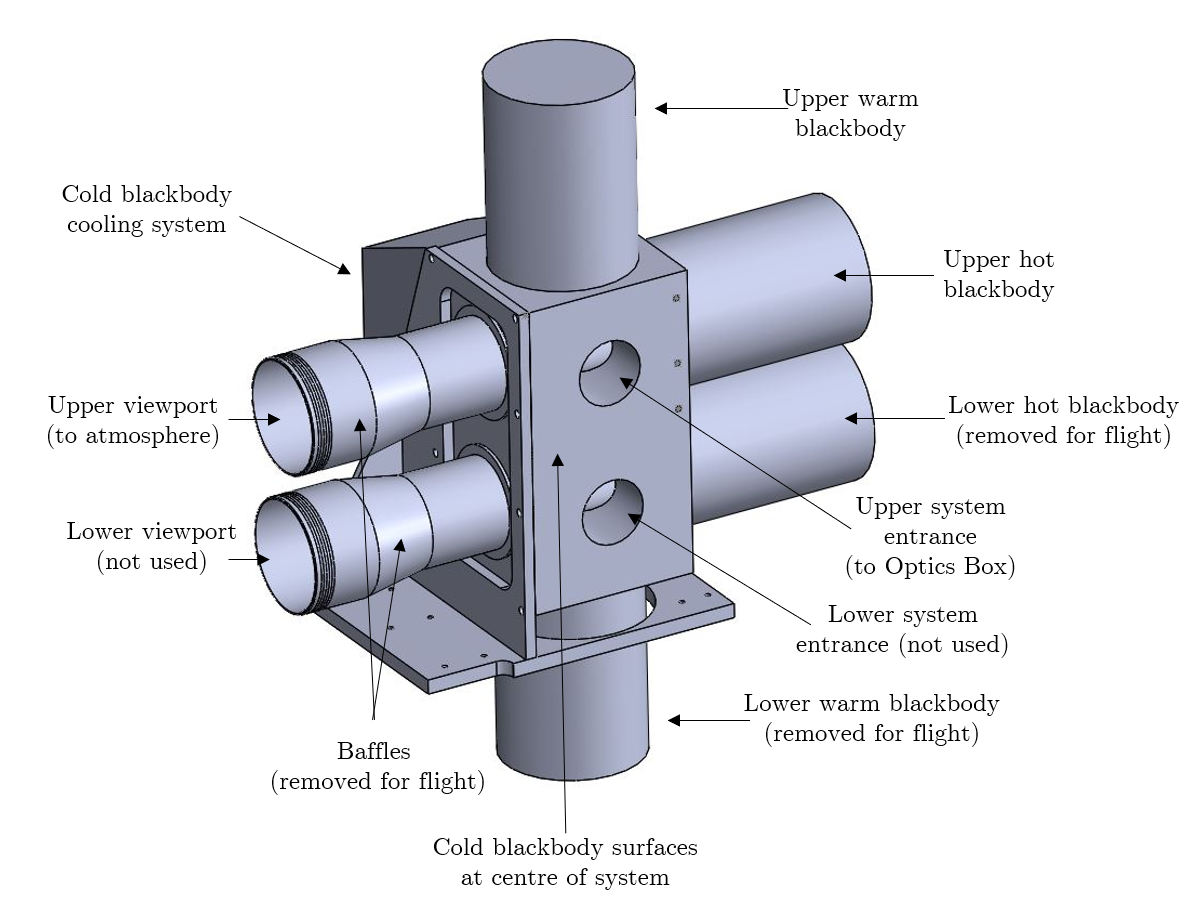
\includegraphics[width=\linewidth]{chap3_images/Blackbody_CAD_labelled_PNG.png}
    \caption{CAD model of LIFE blackbody system.}
    \label{fig:CAD_Blackbodies}
\end{figure}

The temperatures in the schematic show the temperatures from the original configuration, not the LIFE configuration. Also, for the final flight configuration of LIFE, it is noted that the bottom warm blackbody and the bottom hot blackbody are removed, as they are only used for lab verification and are unnecessary weight. Plates were built and installed to cover the openings into the system left by removing these two blackbodies, to ensure that the surfaces remained clean.

The blackbody system operates using a rotating mirror at the centre of each system. The optical path goes through the input window, and reflects off the mirror in whichever direction is necessary: Up for warm blackbody, right for hot blackbody, down for cold blackbody, or left towards the atmosphere. The optical properties of this mirror are unknown, which caused some uncertainty in the self-emission calculations. However as it has a gold coating and was used in a previous application where self-emission minimization was also important, it is assumed to be low. The operation of the mirror was done by rotating a stepper motor, which was one of the first parts of the system to be reconfigured for LIFE. Software needed to be developed to control the stepper motor; this was first done in the proprietary software interface for the particular stepper motor, which was used for all testing and development. Later, in-house software was developed using C++ to allow more direct control and avoid the use of the interface. 

The accuracy of the stepper motor also needed to be verified for proper data analysis after flight. To allow retrievals of the data, a very precise knowledge of the viewing angle of the instrument is needed, to within 0.1°. As there was no encoder for the stepper motor, it was impossible to tell through data feedback where the motor exactly was. Numerous measurements needed to be taken to see the variation in angle each time the mirror realigned itself to image a blackbody or the atmosphere. This also led to the discovery of a few systematic errors, such as the motor overshooting its required stopping position by a certain number of steps. Through testing and development of the motor, this systematic error was corrected, and the error in angle was deemed to be within the 0.1° required.

The largest issue with the blackbody system that required correction were the surface temperatures. Although the surface temperatures of the blackbodies were not important to the detector characterization, as long as they were well known and replicated in all images, the temperature drift over time of the surface was. The LIFE FTS system requires 2.3 seconds to take a full image; if the temperature of the imaged surface changes significantly during this time, there are significant errors in the spectral data and the results are meaningless. The blackbody temperatures must be kept as steady as possible during the image capture time, ideally less than 0.1°C of drift. Temperatures of the blackbodies were controlled via Team Wavelength proportional–integral–derivative (PID) temperature controllers, which were able to withstand a vacuum environment with small modifications, and had been used by previous atmospheric research instruments developed by ISAS. It was discovered that when using these controllers with defined setpoints, the temperature would oscillate around the setpoint indefinitely. PID controllers reach their setpoints by oscillating around a setpoint making small corrections, with the oscillations becoming smaller until the steady setpoint was reached. In the LIFE design the setpoints were never reached, and a different size of oscillation occurred for each blackbody: The hot blackbody oscillated by roughly 4°C every ten minutes, while the cold blackbody could oscillate by as much as 25°C in the same time frame. A temperature reading acquired by the hot blackbody temperature controller is shown in Figure \ref{fig:C2H_temp_oscillation} to demonstrate this oscillation.

\begin{figure}
    \centering
    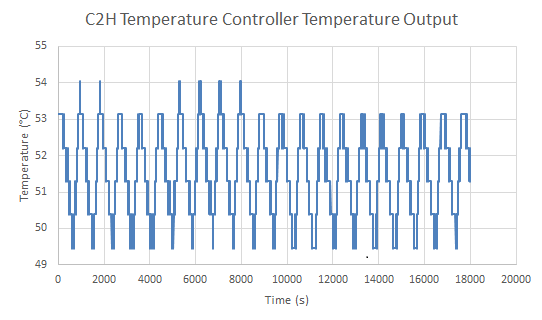
\includegraphics{chap3_images/C2H_temperature_oscillation_excel.png}
    \caption{Oscillation of hot blackbody temperature over 5 hours.}
    \label{fig:C2H_temp_oscillation}
\end{figure}

Often, in a PID system, the oscillation and setpoint overshoot can be minimized by selecting optimized P, I, and D values. In the chosen temperature controller, the only value that allowed direct control was the proportional gain, P. Tests with various values of proportional gain found it to have very little effect on the oscillation error. Eventually it was found through examining documentation and contacting the manufacturer that the integration constant can be changed by changing a specific capacitor. The manufacturer could not provide any guess on what a better capacitance would be, only that it should be lower. Starting with a capacitance of 0.05{\textmu}F, different capacitors were tested with decreasing capacitance. With each decrease in capacitance, the oscillation decreased, but it was not until a 1nF capacitor was used that the error in temperature oscillation was within the required 0.1°C, for the warm and hot blackbodies. However, even at this capacitance, the cold blackbody temperature continued to oscillate by at least 2°C. This problem was eventually solved by using a different temperature controller. This option was not easily available for the other two controllers as they had to be used during flight, needed to be remotely controlled, and be able to survive a vacuum environment. The cold blackbody was only to be used for verification in the lab, so the controller did not have the same requirements. An external controller was sourced, in which the PID values could be easily configured. Through further testing, the values were optimized such that the oscillation of the cold blackbody surface was 0.1°C. With the temperature drift requirements met for all three blackbodies, the blackbody system was fully ready to be used for LIFE.

\subsection{LIFE Preliminary Design: Version 1} 
Prior to the beginning of this thesis, Ethan Runge had planned to develop the thermal-mechanical design himself as part of his MSc. Eventually, it was decided that due to the required amount of work for the design, it should be a separate thesis. However, prior to this decision and prior to this work, a first preliminary version was developed. A large part of Ethan's MSc. thesis was the development of the LIFE optical system, and a CAD model of this system had already been developed in SolidWorks partly through some of Ethan's work and partly from models sent by ABB. This was placed into two early versions for the optics and electronics boxes, both known as Version 1. Though these models would be eventually redesigned from the ground up (besides the core optical system) as part of this thesis, it is helpful to examine this initial design as it would inform the basic concept of future designs. A model of LIFE Version 1 is shown in Figure \ref{fig:LIFE_V1}.

\begin{figure}[h]
    \centering
    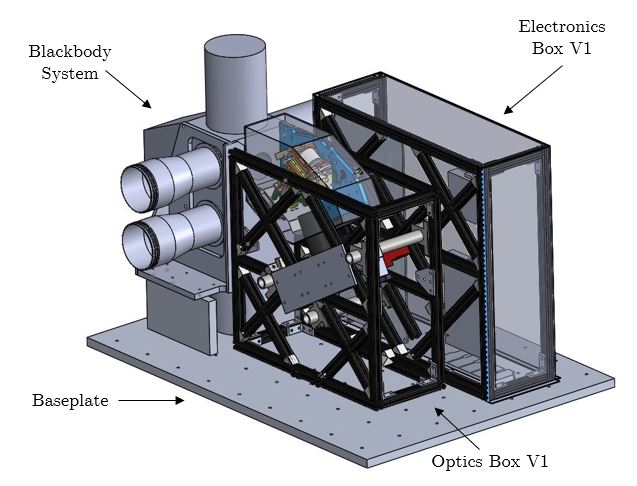
\includegraphics[width=0.8\linewidth]{chap3_images/LIFE_V1_images/LIFE_V1_labelled.JPG}
    \caption{LIFE Version 1.}
    \label{fig:LIFE_V1}
\end{figure}

The layout of this design is the basis of the layout of all subsequent designs: a baseplate with the blackbody at the front, a box containing the core optical system, and an electronics box that contains the optics electronics. However, this is the only aspect of the design that does not change through the subsequent iterations and updates. This footprint is heavily based on the requirement that the MCT Detector be tilted 90° relative to the horizontal, which is described in the next section.

\subsubsection{Optics Box Design: Version 1}
The driving requirement behind the Optics Box design where the optical system is mounted perpendicular to the baseplate is the orientation of the MCT detector pixels. To vertically profile the atmosphere as required, the pixel array needed to be vertical. However, the detector that is supplied with the FTS system has a horizontal 1x16 pixel array. As a result, it needed to be mounted on its side, such that the horizontal array would be turned vertical, and the atmosphere could be vertically resolved. Mounting the optical system perpendicular to the baseplate was a break from all previous instruments that the ISAS atmospheric research group had designed, and led to increased complexity in development. This complexity would lead to issues such as needing to be mounted to the wall, yet have all parts be free to move if necessary for alignment, and still be sturdy enough to avoid any shaking causing misalignments during the flight. Version 1 of the Optics Box, designed to meet the requirement of tilting the optical system, is shown in Figure \ref{fig:OB_V1}.

\begin{figure}
    \centering
    \begin{subfigure}[h]{0.4\textwidth}
        \centering
        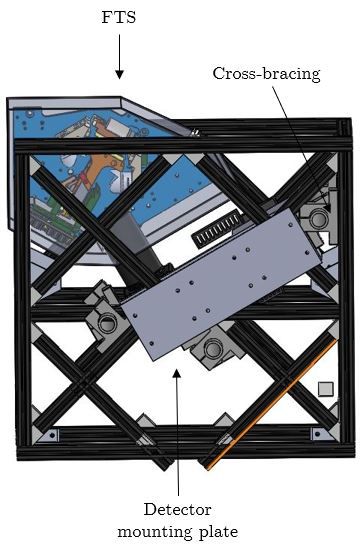
\includegraphics[width=\textwidth]{chap3_images/LIFE_V1_images/Optics_Box_V1_V0_front_view_labelled.JPG}
        \caption{Front view of Optics Box V1.}
        \label{fig:OB_V1_front}
    \end{subfigure}
    \begin{subfigure}[h]{0.42\textwidth}
        \centering
        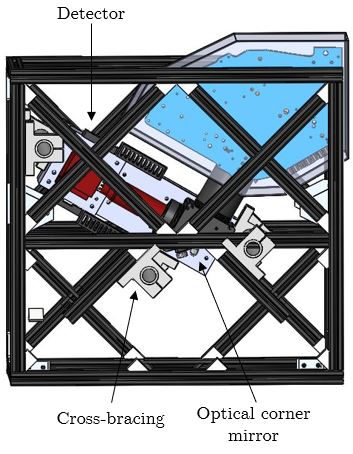
\includegraphics[width=\textwidth]{chap3_images/LIFE_V1_images/Optics_Box_V1_V0_rear_view_labelled.JPG}
        \caption{Rear view of Optics Box V1.}
        \label{fig:OB_V1_rear}
    \end{subfigure}
    \caption{Original design of the Optics Box.}
    \label{fig:OB_V1}
\end{figure}

The initial design used a construction material known as \textit{T-frame}. It is an inexpensive, off-the-shelf component made from aluminum that is designed to easily fit together and also comes with fasteners and connectors, all readily available and easy to build. Being able to order this material and build in-house would save a large amount of the construction budget. It also still allowed freedom in the design, as all components could be cut to length as necessary. Using a CAD model of this material taken from a suppliers website, a model for the box could be quickly designed. However, downsides to this material was that although easy to build, it is not entirely secure, as a result of manufactering tolerances. Connecting things to this frame would also be a challenge, as there was no easy way to mount any parts, such as the FTS, to the wall, without having either an interface plate or to install it prior to putting the box together, which meant a significant amount of time could be necessary for repairs.

Initially, as described in Section \ref{electronics_reqs}, vibration needed to be dampened as much as possible. Vibrations from the Stirling cooler could potentially cause vibrations in the FTS, which would cause errors in the data. The solution to this was to use a spring system between the detector and the wall of the box, which would dampen the vibrations enough that they would not travel to the FTS system. These springs cannot be seen in Figure \ref{fig:OB_V1} but are between the detector mounting plate and the detector. The box was further stiffened through the use of rods connecting the two walls of the box, to try to avoid vibrations propagating freely through the T-frame structure, either from the detector or from the gondola.

When I began my thesis, and took over the mechanical design, one of the first design decisions made was that the vibrations were not going to be as much of an issue as originally thought. As a result, the spring system and cross-braces were removed. A Version 1.1 was developed, which was a simplified version of the original design with the optics attached to the walls through an interface plate, and other unnecessary stiffening and dampening components removed. An updated model of this design is shown in Figure \ref{fig:OB_V1.1}.

\begin{figure}
    \centering
    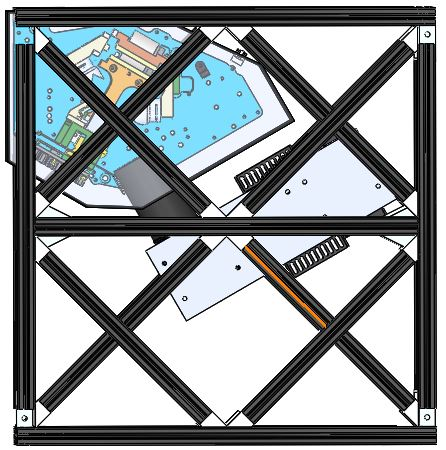
\includegraphics[width=0.5\textwidth]{chap3_images/LIFE_V1_images/Optics_Box_V0_5_front_view.JPG}
    \caption{Version 1.1 of the Optics Box, with dampening and cross-bracing components removed.}
    \label{fig:OB_V1.1}
\end{figure}

One of the main issues of this design is that it is open; the optics must be kept as clean as possible, and need to be well protected when not in a clean room. In addition, thermal control of the optics would be easier if the entire temperature environment inside the box could be kept steady. Therefore, the main requirement of the next version of the optics box would be to design an enclosure for the optics, in a way that would enclose the optics and FTS while not directly attaching to these components to avoid vibration propagation and to be easier to install around the optics. 

\subsubsection{Electronics Box Design: Version 1}
The design of the Electronics Box changes throughout the design process largely due to two reasons: The thermal requirements, and adding more components. As the mechanical design progressed, so did the electrical design, completed by lab engineer Paul Loewen. This required room for more parts, and the box grew, and parts shifted around. However, for the first design, the only electronics that were of concern were the components necessary for the operation of the optical system: The FTS control board, known as the BMXS board, the two data acquisition boards, with the Pleora Ethernet interface boards attached, an Ethernet hub to allow the data acquisition boards, BMXS board and the external computer to all communicate, and a power supply for the system. An image of Version 1 of the Electronics Box is shown in Figure \ref{fig:Ebox_V1}. Similar to Version 1 of the Optics Box, the original version of the Electronics Box used T-frame as its basic structure. Aluminum panels on all sides, including on the back to which the electronics are bolted, are transparent in the figure so the T-frame and inner electronics can be seen. This is a simple design, and like the Optics Box T-frame, would be easy and inexpensive to build.

\begin{figure}
    \centering
    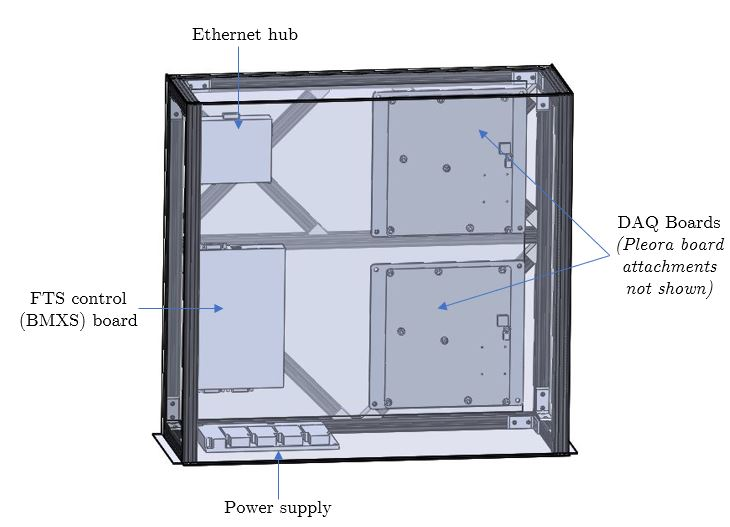
\includegraphics[width=0.85\textwidth]{chap3_images/LIFE_V1_images/Ebox_V1_labelled.JPG}
    \caption{CAD model of Version 1 of the Electronics Box.}
    \label{fig:Ebox_V1}
\end{figure}

Although later in the process the design of the electronics box would be driven by the thermal analysis, the initial design was driven by the cable length connecting the detector and the data acquisition boards. Sixteen cables (one for each detector pixel) sent signals from the detector to these boards, to be amplified, digitized and sent to the computer. These cables were extremely delicate and could not be lengthened; due to the signals being unamplified coming from the detector, they would have to be fed directly from the Optics Box to the Electronics Box. Thus these boards were placed and oriented in the Electronics Box to minimize distance to the detector. The rest of the components were placed around arbitrarily in the rest of the box. The thermal analysis of this box is completed when the first computer stack was developed and added to the design, during the development of LIFE Version 2.

\subsection{LIFE Preliminary Design: Version 2}
The second iteration of LIFE was largely based around a thorough update of the optics box. This was the first major design iteration that was developed as part of this thesis, and was more heavily based on thermal constraints. Design changes are largely based on the results of thermal analyses. The Electronics Box remained largely the same for this iteration, with the exception of adding the computer stack component. However, the initial thermal simulations of the Electronics Box were done in this version as well, and would inform updates of the Electronics Box in future LIFE versions. A full model of LIFE Version 2 is shown in Figure \ref{fig:LIFE_V2}.

\begin{figure} % This may not need to be here, could just skip the full version models
    \centering
    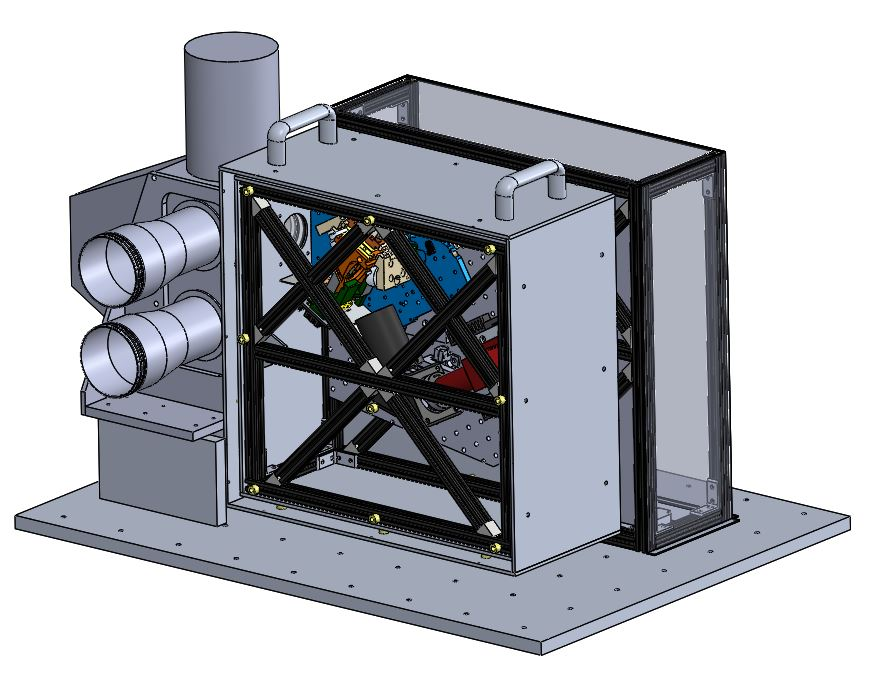
\includegraphics[width=0.8\textwidth]{chap3_images/LIFE_V2_images/LIFE_V2.png}
    \caption{LIFE Version 2}
    \label{fig:LIFE_V2}
\end{figure}

\subsubsection{Optics Box Design: Version 2}
To allow the optics temperatures to be more easily controlled, and to protect the optics when outside of a clean room, a box was designed around the T-frame. It consists of six panels that are bolted directly onto the T-frame structure. In addition to this, the optics system was redesigned to be attached to a single optical breadboard. This breadboard could be attached directly to the T-Frame, so the placement, alignment and testing of all optical components could be done externally outside the box, before a simple installation. In addition, all components would be on one plane inside the box, making final alignment much easier. Having all components bolted to this breadboard also allows a more uniform temperature across all components. With the previous design, different components were mounted on different parts of the frame, meaning multiple heaters, temperature sensors, and controllers would be necessary to ensure that each optical component would remain at the same temperature. Constraining the optical system to one baseplate means easier temperature control, as they are all on one surface, the temperature of which could be more easily controlled. A further change to this design was to make it smaller and cut out unnecessary empty space inside. The height of the FTS is the constraint, as it must align with the entrance of the blackbody system, so there will be an empty area towards the bottom of the box; however the extra space on all sides of the optical system were made smaller. 

Beyond this improvement in the optics and surrounding box, there was still a potential to improve it further.  With the components enclosed in a box, external radiation, either from the environment (e.g. sun) or from nearby components (e.g. Electronics Box), could warm the box and cause the system to overheat. An idea was taken from the CATS instrument design, which had similar requirements for temperature: External walls, known as radiation plates, can be placed as an outer layer over the inner box. To prevent any thermal path between the internal and external walls, titanium spacers are used as a connection between these plates, which have a low thermal conductivity. Thus, in a vacuum environment, heat can only be transferred through radiation from the exterior plates to the interior plates, and through conduction through the spacers. Heat transfer through both of these paths are very slow. This allows the inner box to stay at a steadier temperature, minimizing any external temperature variations that may occur. This design also added titanium spacers as an attachment between the Optics Box and the baseplate. The gondola temperature can swing as low as -50ºC, and this limits large temperature oscillations and temperature drops as a result inside the optics box. Smaller heaters can then be used to keep the optics above the minimum temperature requirements. The finalized model for the Optics Box Version 2 is shown in Figure \ref{fig:OB_V2}.

\begin{figure}
    \centering
    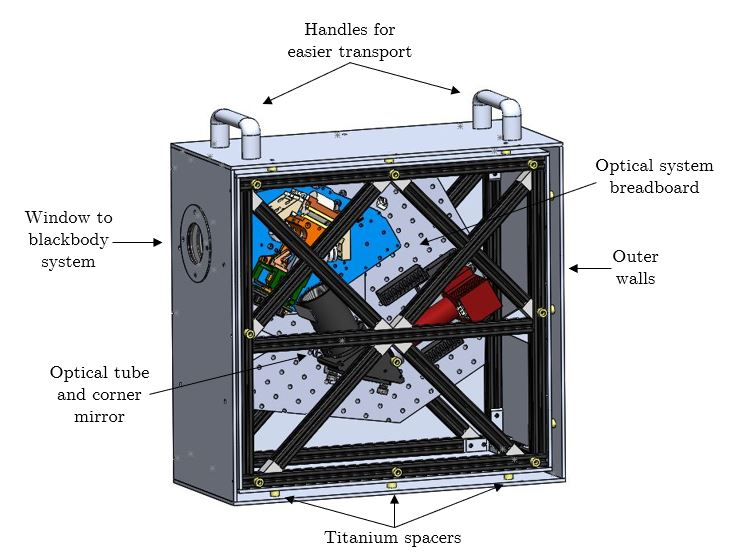
\includegraphics[width=0.84\textwidth]{chap3_images/LIFE_V2_images/Optics_Box_V1_labelled.JPG}
    \caption{Version 2 of the Optics Box, which incorporates external radiation plates.}
    \label{fig:OB_V2}
\end{figure}

This was the first component of the instrument to be studied with thermal analysis. As this design was created with thermal properties in mind, it was important to see the results of using these various design methods to help with the thermal analysis. There are four main heat loads for the thermal analysis of this box: The dissipated heat of each electrical component, the temperature of the base of the box (i.e. gondola temperature), the temperature of the side wall caused by the electronics box, and the power of the resistive heaters applied to the plate. The dissipated heat of each electrical component is known, and given by ABB: The FTS generates a negligible amount of heat (1W chosen for study) and the MCT generates 8W. The baseplate temperature was changed between -30°C and -20°C. The side wall heat load was assuming a thermal connection between the electronics box and optics box, as a way to dump heat from the electronics box and warm the optics box. The final heat load, the heaters, is unknown and iterated through the design to meet the temperature requirements. A total of 17 designs were simulated, each with a different amount of heaters, placement of heaters, and power dissipated from the heaters. For each simulation, temperatures of various components were measured, such as the FTS, different parts of the breadboard, the lens system, and an average temperature of the breadboard, outer and inner walls. These were recorded in a spreadsheet describing the results of each simulation to track the changes through simulation iterations. Only a few of these iterations will be described here.

It is noted that the majority of the initial simulations, until later in the design process, were steady-state. SolidWorks has the ability to perform transient analysis, and is utilized for the final designs, but to perform these simulations it must complete a simulation for each time step. As a result, the time to solve a transient analysis can be very long, and it was not realistic to perform this for rapid prototyping. Through some transient analysis tests, it was found that many hours were required to actually reach steady state temperatures ($>$12 hours), longer than the time of flight. As such, the steady state temperatures are the maximum or minimum temperatures that will be reached, and can be treated as worst-case scenario results. If the temperatures from a steady-state simulation fit within the temperature requirements, it will certainly reach those requirements for the transient analysis and during the flight time frame.

The initial simulation involved no heaters, as a test to see how cold the optics would get with a -30°C baseplate. The majority of the heat comes from the Electronics Box, based on an idea that the Electronics Box and Optics Box could be thermally connected, as a way to use the waste heat from the Electronics Box and make the instrument more efficient. The result of this simulation is shown in Figure \ref{fig:OB_V2_TA_1}. 

\begin{figure}
    \centering
    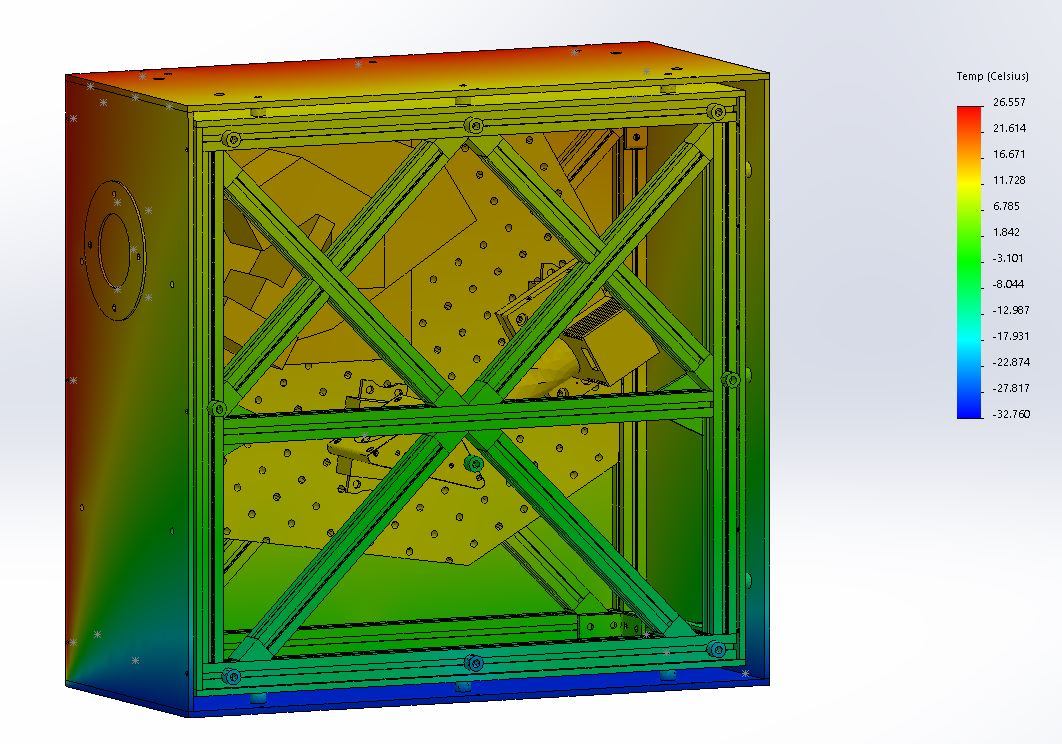
\includegraphics[width=0.8\textwidth]{chap3_images/LIFE_V2_images/Thermal_Analysis_25_deg_-30_deg.JPG}
    \caption{Initial temperature simulation of Optics Box V2, with no heaters and a direct connection to the Electronics Box.}
    \label{fig:OB_V2_TA_1}
\end{figure}

A key takeaway from this simulation is that the titanium spacers are accomplishing their task of minimizing the cold travelling through the bottom of the box into the optical system. With a spacer of roughly 1cm in height, there is a temperature change of almost 20°C. The temperatures of the optical system are in a range of 12-15°C, on the low end of the required temperature range, and is dependent on heat coming from the Electronics Box. As a way to increase the temperature for the next test, the outer radiation plate between the optics and electronics boxes is removed. This allows a more direct heat path between the boxes with the removal of the titanium spacers, and will further warm the optics box. The results of this simulation is shown in Figure X\ref{fig:OB_V2_TA_2}

\begin{figure}
    \centering
    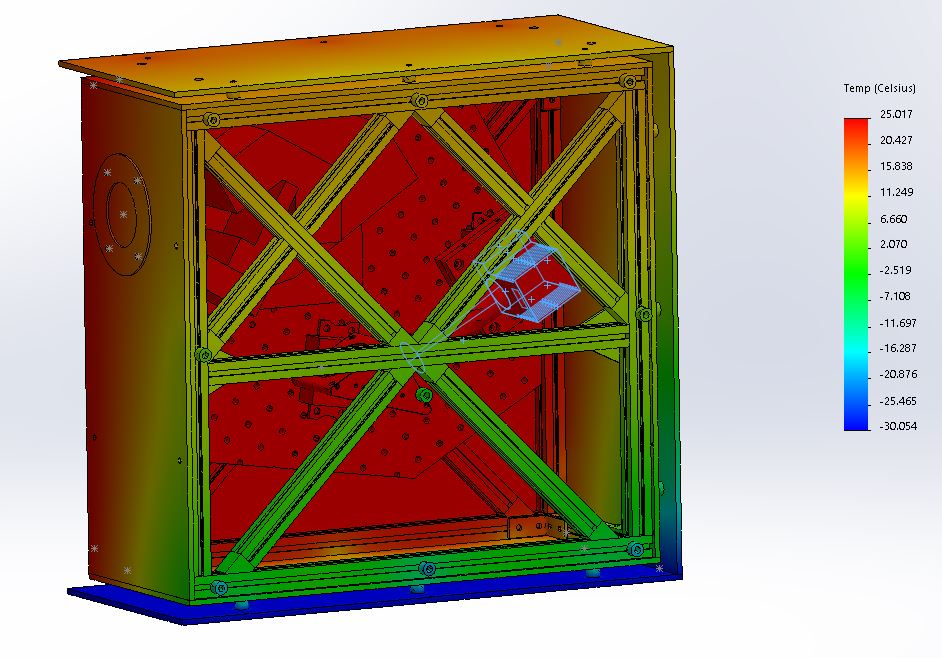
\includegraphics[width=0.8\textwidth]{chap3_images/LIFE_V2_images/TA_25_-30_no_front_left_outer_walls.JPG}
    \caption{Simulation of Optics Box V2 without an outer wall between the Optics Box and Electronics Box.}
    \label{fig:OB_V2_TA_2}
\end{figure}

The result, as expected, is that the optical system is much warmer. With a direct path to a 25°C source, much of the optics come close to 25°C. The temperatures of the optics are at the high end of the required temperature range, and ideally should be more towards the centre. However, the biggest issue with this design is that the temperature of the optics are based heavily on the temperature of the Electronics Box, which cannot be controlled as it is simply heat being dissipated from the electronics. There should be a better method of control than relying on this heat, so heaters are added to the design. For the next simulation, the outer wall is added back, so the temperature from the Electronics B=ox will be closer to what is seen in Figure \ref{fig:OB_V2_TA_1}. For this test, the heaters are all set to 30W, and the resulting simulation is shown in Figure \ref{fig:OB_V2_TA_3_3HEATERS}.

\begin{figure}
    \centering
    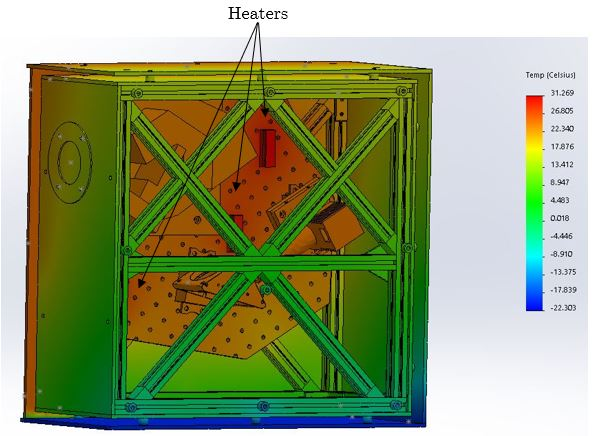
\includegraphics[width=0.8\textwidth]{chap3_images/LIFE_V2_images/TA_25_-20_no_front_wall_three_heaters_labelled.JPG}
    \caption{Simulation of Optics Box V2 with three heaters at 30W.}
    \label{fig:OB_V2_TA_3_3HEATERS}
\end{figure}

The temperatures of the core components of the FTS and lenses are now roughly 23°C. It is on the high end of the temperature range but the power to the heaters can be controlled by turning them off if the temperature of the optics gets too high; thus the maximum temperature they will reach is 23°C. This design satisfies the temperature requirements. However, these temperatures are still assuming a constant temperature of 25°C from the Electronics Box. If the electronics were not dissipating as much power as expected, this temperature would fall, potentially causing the optics to fall below 5°C. To see what would happen if this temperature connection was removed, thus allowing full control of the optics just through heaters, a simulation was done with no temperature condition on the side wall. To compensate, an extra heater was added on the optics plate. Through a few iterations, the heat powers also had to be increased to allow the optics to stay within their required ranges: 25W for the heater attached to the FTS, and the three heaters attached to the breadboard are 100W, 50W, and 25W. The results of this simulation is in Figure \ref{fig:OB_V2_TA_4_4HEATERS}.

\begin{figure}
    \centering
    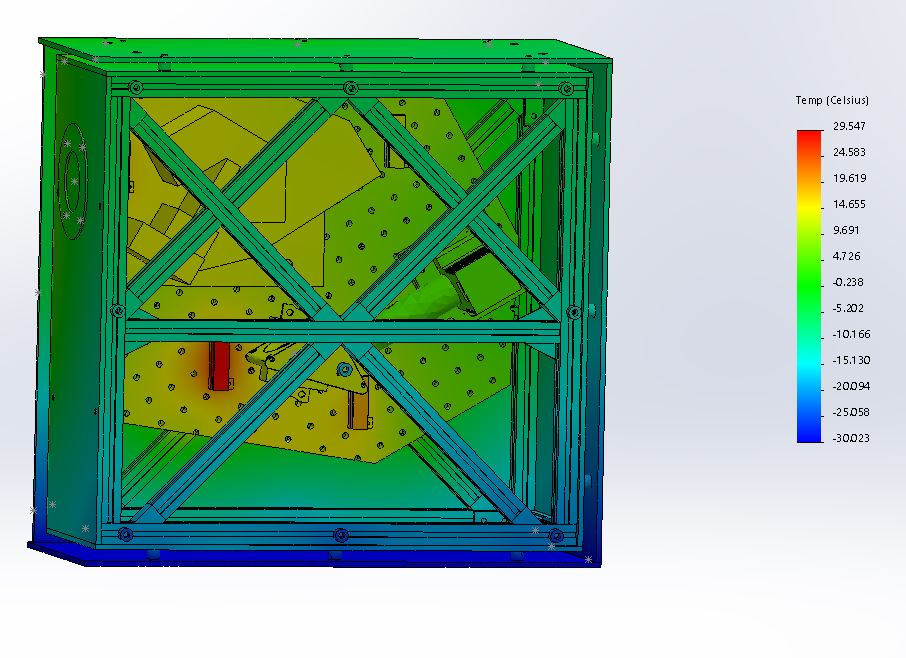
\includegraphics[width=0.8\textwidth]{chap3_images/LIFE_V2_images/TA_-30_no_front_wall_four_heaters.JPG}
    \caption{Simulation of Optics Box V2 without any heat flow from the electronics box, and four heaters.}
    \label{fig:OB_V2_TA_4_4HEATERS}
\end{figure}

These temperatures are in the required temperature range. However, just to maintain minimum allowable temperatures, the total power for the heaters was 200W, which is far beyond the reasonable power limit to just heat the Optics Box. To ensure a more reasonable power draw, the best option would be to transfer heat from the Electronics Box. However, another method to better control the optics temperatures is explored in the next version of the Optics Box.

In addition to the issues with trying to maintain proper Optics Box temperatures, there is an issue with the mechanical design. It was discussed that the cost savings of the T-frame may not be worth the difficulties that come with it. It will be difficult to align all connections properly after building the T-frame, due to its loose tolerances, and in addition it is difficult to attach the plates to the frame, where a special screw attachment is needed, and attaching it through various panels could prove difficult. A new version of the Optics Box would later be created that removed the T-frame structure, to allow for easier construction.

\subsubsection{Electronics Box Design: Version 1 Thermal Analysis}
This Electronics Box overall design remained largely unchanged in Version 2 of LIFE, but the initial thermal simulations were completed here, after the thermal simulations of the Optics Box Version 2 as described above. The main change before simulations was the addition of the LIFE \textit{Computer Stack}, the computer control centre of the instrument. This does not have stringent temperature requirements and does not dissipate a large amount of heat so does not have a large affect on the design, but must be considered for the purpose of space. As discussed in Section \ref{electronics_reqs}, most electronics have narrow temperature ranges and simulations must be completed to ensure that they will stay within these ranges during flight and in the lab.

Initial simulations were completed with each part dissipating typical heat power, and the baseplate temperature was kept at -20°C and is changed to more extreme temperatures in later tests. The first thermal test of the Electronics Box with these constraints is shown in Figure \ref{fig:EBOX_V1_TA_1_SQUARECENTRE}. The main issue with this design is that there is not enough heat being dissipated from the DAQ boards, and the temperature reaches 51°C in the top right corner, which is above the maximum operating temperature of 45°C. The design must be altered so that more heat can be dissipated to the gondola deck. To do this, the baseplate which the electronics are mounted to was made larger, extending out to the edge of the T-frame. This allowed more thermal contact with the structure so that more heat could dissipate into the frame, which could dissipate into the gondola deck. The results of this change are shown in Figure \ref{fig:EBOX_V1_TA_2_BIGGERCENTRE}.

\begin{figure}
    \centering
    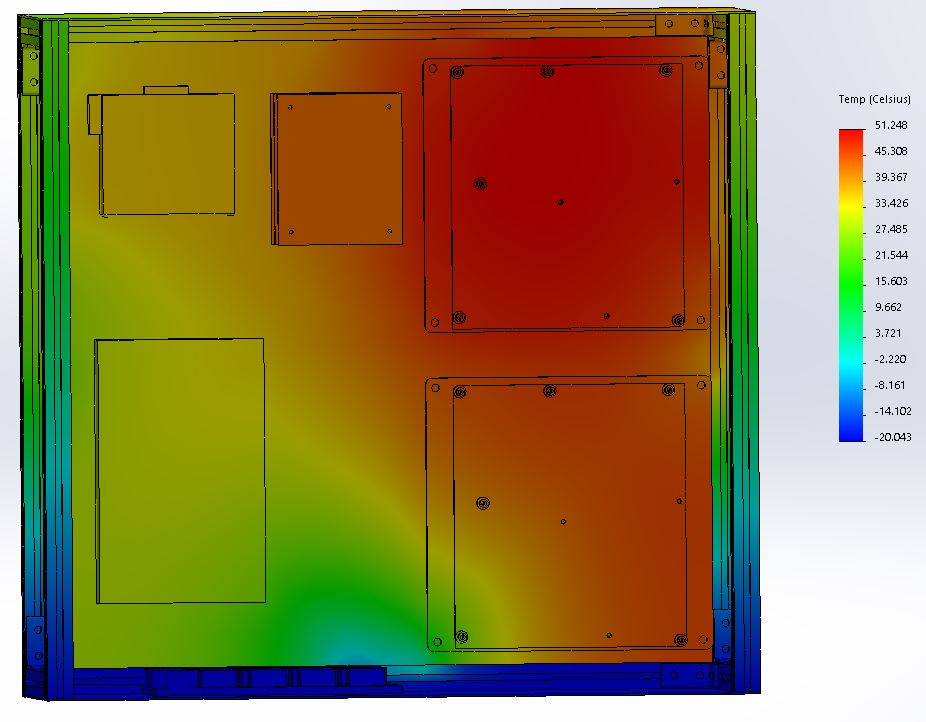
\includegraphics[width=0.7\textwidth]{chap3_images/LIFE_V2_images/TA_-20_square_centre_plate.JPG}
    \caption{Initial thermal simulation of Electronics Box V1, with a base temperature of -20°C.}
    \label{fig:EBOX_V1_TA_1_SQUARECENTRE}
\end{figure}

\begin{figure}
    \centering
    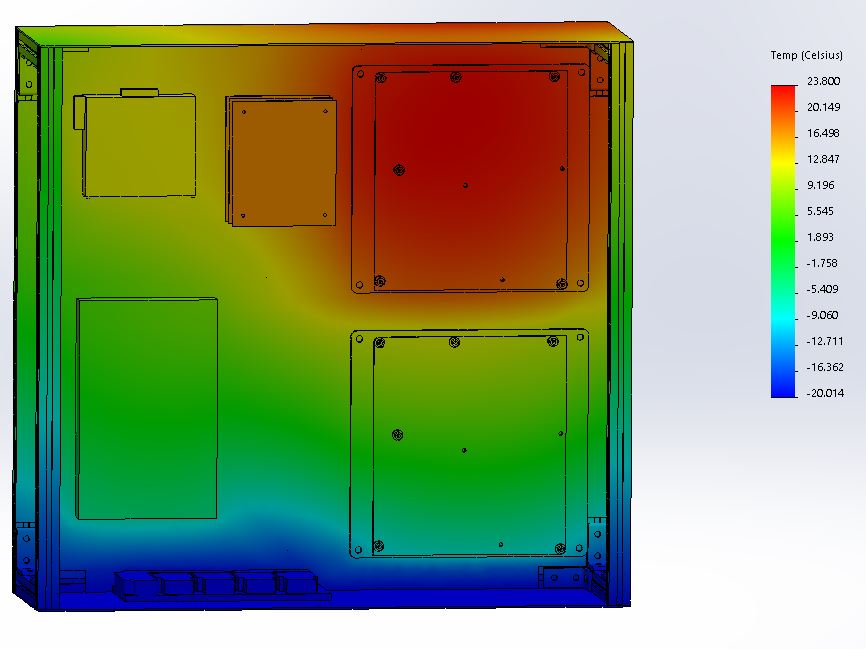
\includegraphics[width=0.8\textwidth]{chap3_images/LIFE_V2_images/TA_-20_expanded_centre_plate.JPG}
    \caption{Second thermal simulation of Electronics Box V1, with an expanded electronics mounting plate.}
    \label{fig:EBOX_V1_TA_2_BIGGERCENTRE}
\end{figure}

In this model, the temperatures of the upper DAQ board is improved to be within a reasonable range, but now the lower DAQ board (on the bottom right) and the BMXS board are now dangerously close to their minimum temperature limits, as the cold from the gondola makes better contact with the electronics baseplate. This would be a recurring problem with the design of the electronics box; the DAQ board dissipate a high amount of power, and to avoid overheating, this power needs to be dissipated to the gondola baseplate. However, with a large thermal connection to the baseplate, the electronics become too cold, as the minimum temperature value of the DAQ board is 0°C and the minimum value for the BMXS board is 5°C. It is unlikely that this design would have survived the extreme temperatures of the ascent. The further development of this thermal model to address these issues is done alongside the development of the Optics Box thermal model, and in subsequent chapters are discussed together. 

\subsection{LIFE Preliminary Design: Version 3}

Similar to Version 2, the main change in Version 3 of LIFE was a widespread update to the Optics Box. It was designed around the need for something easier to build, and is further based upon the CATS design. On the other side of the instrument, the Electronics Box received minor updates, adding electronics and further altering the design to improve the thermal properties of the instrument. A more thorough update of the electronics box occurs in Version 4 of the instrument. A model of Version 3 of LIFE is shown in Figure \ref{fig:LIFE_V3}.

\begin{figure}
    \centering
    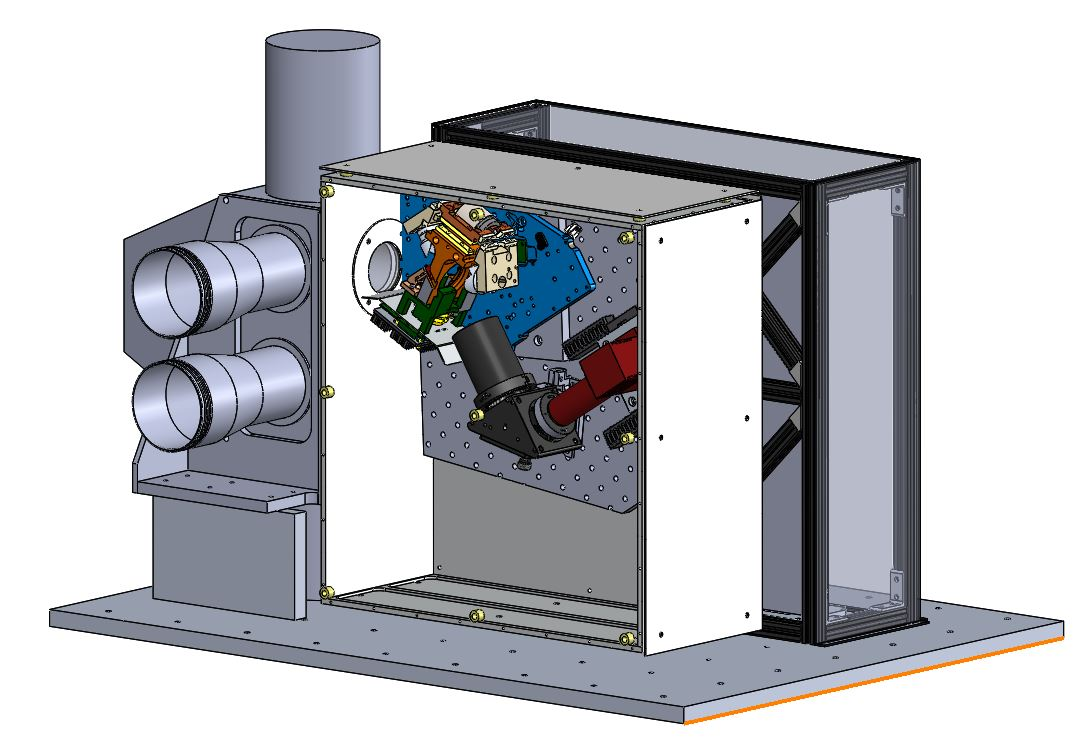
\includegraphics[width=0.7\textwidth]{chap3_images/LIFE_V3_images/LIFE_V3.JPG}
    \caption{Third version of LIFE, with an updated optics box.}
    \label{fig:LIFE_V3}
\end{figure}

\subsubsection{Optics Box Design: Version 3}
Although the previous version of the Optics Box met most of the requirements, such as the proper temperature range in different scenarios and holding a steady temperature, there were still some downsides to the design. Chiefly, there was the issue of it being very difficult to assemble. Although the costs were kept low by buying a number of off-the-shelf components and keeping the cost of having the components made by the machine shops low, it would be tough to maintain. With the T-frame design, all walls would have to be bolted to the T-frame, which would be a more difficult task once the instrument was more fully enclosed. It would be even more difficult when attaching the outer radiation plates through the inner walls, where the bolts would have to be connected blindly. In addition to attaching plates, it would be difficult to attach the optics breadboard baseplate to the wall, as it would need to be done from the optics side (hence the bolts could not be in the optical path, and would also lead to a risk of bumping the optics). Finally, the largest issue would be the need to perform fixes, alignments and maintenance to the optical system when it was fully built. The T-frame would need to be removed from one side of the box to allow access, which would be difficult, time intensive, and difficult to reinstall without altering the optical setup.

After discussions with the rest of the LIFE team, it was agreed that a trade-off of higher cost would be reasonable for a design that was easier to build and access. Thus, a new design was developed from the ground up, only keeping the core optics system the same. The new design was further developed from CATS: The walls would be thicker and all walls could be directly bolted together, thus only needing six parts for inner walls, and removing the need for any inner structure. The outer radiation plate design would be kept the same, but would be easier to install as the outer plates could be attached directly to the inner plates. The optical system baseplate could be directly bolted to the wall from the opposite side of the optics. If the optics needed to be aligned or otherwise worked on, the entire baseplate could be disconnected from the other side and lifted out, or only one side of the box would need to be removed to have access, rather than one side plus the T-frame bracing. A model of the third version of the Optics Box is shown in Figure \ref{fig:OB_V3}. 

\begin{figure}
    \centering
    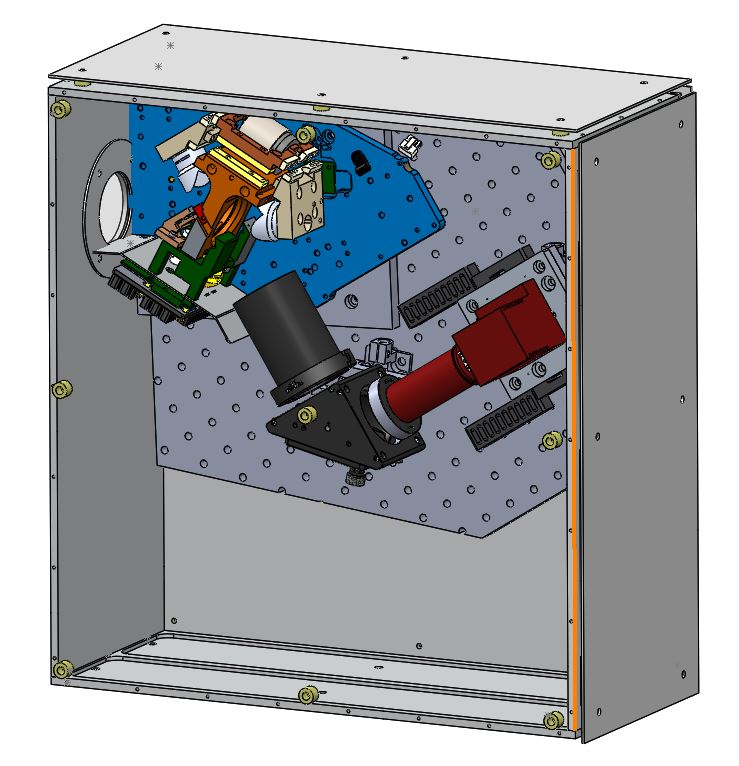
\includegraphics[width=0.7\textwidth]{chap3_images/LIFE_V3_images/Optics_Box_V2.JPG}
    \caption{Third version of the Optics Box, based on the CATS design.}
    \label{fig:OB_V3}
\end{figure}

The two main drawbacks to this new design was expense and weight. The weight was minimized by milling cavities from the thicker panels, and the cover plate was chosen to be as thin as possible (the backplate was thick and not milled out to be able to hold the weight of the optics system). All parts for this new design would need to be built by the machine shops, which caused a threefold increase in price. However it was decided that this design was worth the cost, and would be the core design for the rest of the design iterations.

For the thermal analysis of this version, the core aspects of the thermal design are still present: The titanium spacers and radiation plates. However as the walls are rigidly connected together and there is no frame, heat would flow differently. Another change from the previous design is leaving gaps between the radiation plates, which removes heat flow between these plates and  better isolates the interior. Once again, there were a large number of thermal simulation iterations, and only a select few will be discussed here.

Initial simulations for this box still assume a thermal connection between the Optics Box and Electronics Box, so the outer radiation plate that faces the Electronics Box is set as 25°C. In this simulation, although all heaters are still in the model from Optics Box Version 1, only one is dissipating power (the bottom right), at 12.5W. The bottom plate is set at a temperature of -20°C. The FTS and MCT Cooler are dissipating their normal heat loads. The results of this simulation can be found in Figure \ref{fig:OB_V3_TA_1}.

\begin{figure}
    \centering
    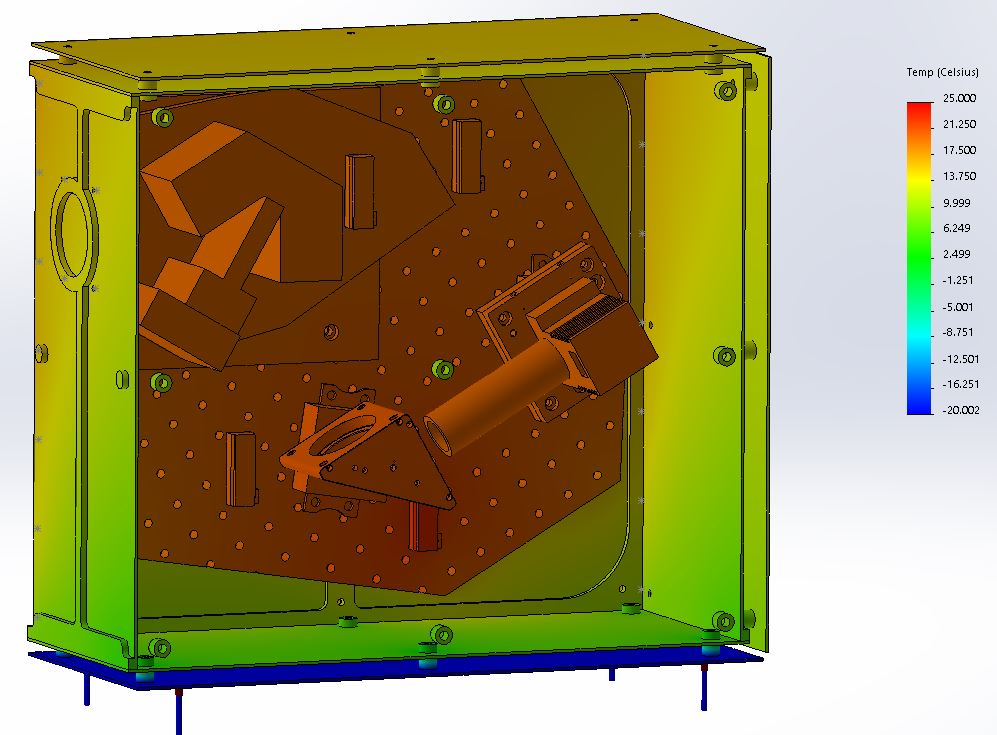
\includegraphics[width=0.8\textwidth]{chap3_images/LIFE_V3_images/TA_-20_deg_20_deg_12W_heater.JPG}
    \caption{Simulation of Optics Box V3 with a heater and thermal connection to the Electronics Box.}
    \label{fig:OB_V3_TA_1}
\end{figure}

The most important outcome of this simulation is it shows the effect of heat flow compared to the previous version. With a 12.5W heater and heat dissipated from the electronics box, the temperatures are staying within their required limits, as compared to heat power of over 100W needed for the last simulation with T-frame. The titanium spacers are still performing well in maintaining steady temperatures and isolating the inner box from the gondola baseplate. The next simulation shown is with no thermal connection between the Electronics Box and Optics Box, to allow better thermal control without relying on heat coming from the electronics, which cannot be actively controlled. With only the top right heater being used with a power dissipation of 35W, Figure \ref{fig:OB_V3_TA_2} shows the resulting simulation with a baseplate temperature of -30°C (extreme cold case).

\begin{figure}
    \centering
    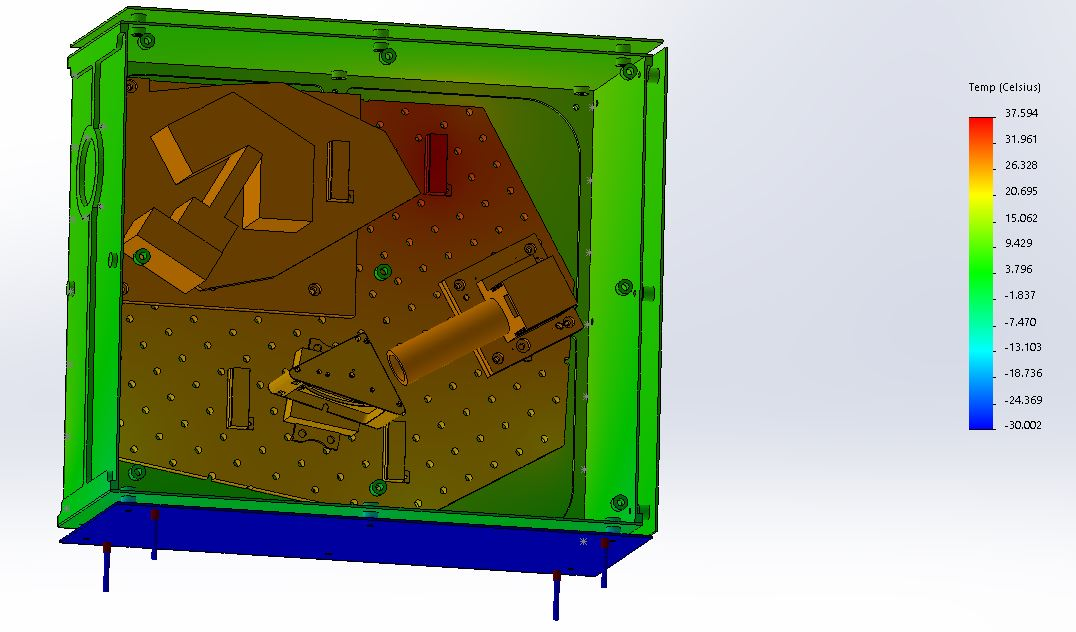
\includegraphics[width=0.8\textwidth]{chap3_images/LIFE_V3_images/TA_-30_deg_35W_heater.JPG}
    \caption{Simulation of Optics Box V3 with no thermal connection to the Electronics Box.}
    \label{fig:OB_V3_TA_2}
\end{figure}

The temperatures are above their temperature ranges, even with the -30°C baseplate, which is good. Although the temperatures are too high, with a properly controlled heater this will stay within its temperature limits. Further iterations can be completed to see exactly what heater power is required. However, although this system works, one more thermal control method is implemented. Currently, although the inner Optics Box stays at a relatively uniform temperature due to the titanium spacers and outer radiation plates, it can still incur larger temperature oscillations than required for good optical operation. To prevent this and better isolate the optics, titanium spacers are added between the optics breadboard and the Optics Box wall. This is one of the most important parts of the thermal system to ensure a steady temperature in the optics, as it further decreases temperature oscillations as a result adding another thermal insulation layer. Also, it allows for a more uniform temperature across the whole system, allowing for further ease in removing the self-emission, and also lowers the necessary heater power as the heat can only escape through radiation. With the titanium spacers in place, a simulation is performed with a heater power of 20W and a baseplate temperature of -30°C, shown in Figure \ref{fig:OB_V3_TA_3_SPACERS_ADDED}.

\begin{figure}
    \centering
    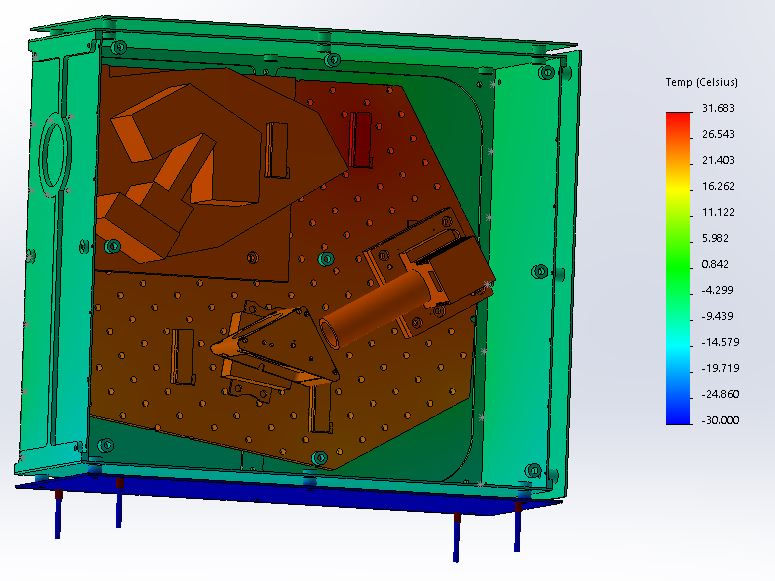
\includegraphics[width=0.8\textwidth]{chap3_images/LIFE_V3_images/TA_-30_deg_20W_heater_isolated_board.JPG}
    \caption{Simulation of Optics Box V3 with titanium spacers added between the optics breadboard and the side wall.}
    \label{fig:OB_V3_TA_3_SPACERS_ADDED}
\end{figure}

This model shows that the titanium spacers do have a signification effect. The temperatures of the optics are the similar to the previous simulation, but with 15W less heater power necessary. The temperature of the optics has less dependence on the gondola baseplate temperature as well. Overall this design is much improved over the previous design, using much less heater power while keeping temperatures more steady, and also being easier to build. This is the last major update for the Optics Box overall design, but further temperature simulations are done as part of the larger LIFE assembly, which includes the Electronics Box. This begins in Version 4 of the instrument.

\subsection{LIFE Preliminary Design: Version 4} 
The next version of LIFE is largely based around a thoroughly redesigned Electronics Box. This is also the first version to simulated both the Optics Box and Electronics Boxes together as a full assembly. As there is no major updates to the Optics Box, there will only be a discussion of the redesigned Electronics Box before going into the full assembly thermal simulations.

\subsubsection{Electronics Box Design: Version 2}
The previous version of the Electronics Box had the same design issues as the first two versions of the Optics Box, which was the use of T-frame. As in the Optics Box, the use of T-frame to build the Electronics Box, although inexpensive, would have been difficult to build well, and the thermal design more difficult. As a result, the Electronics Box was redesigned from the ground up using a similar design to the Optics Box, using CATS as inspiration. The box would now be made from machined aluminum panels, which would connect to each other directly, so that an inner frame did not need to be used. To save weight, the side panels had milled cavities. The heaviest part of this new design was the mounting plate for the electronics, the thickness of which was based on both the strength needed to mount the electronics securely, as well as dissipate heat effectively. This version still only contains the core electronics at this point; the next version of the box contains the rest of the necessary components. The layout of the electronics remains the same as the previous version, with the exception of the power supply, as a result of the mounting holes on the bottom plate. This model is shown in Figure \ref{fig:EBOX_V2}.

\begin{figure}
    \centering
    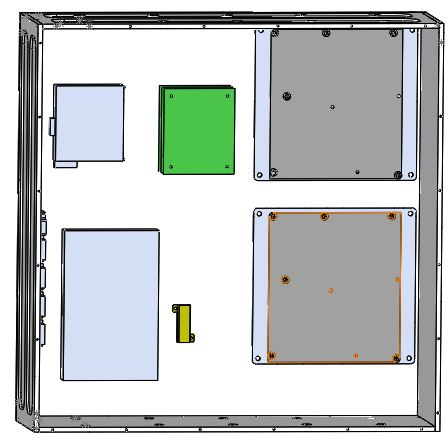
\includegraphics[width=0.7\textwidth]{chap3_images/LIFE_V4_images/Ebox_V2.JPG}
    \caption{Second version of the electronics box, following the design of the Optics Box.}
    \label{fig:EBOX_V2}
\end{figure}

The thermal analysis of this box was done as a full assembly with the Optics Box. However it is noted that there is now a better thermal connection between the box and the gondola deck. As a result, the heat from the DAQ boards can dissipate easily into the gondola deck, but in the cold case the BMXS and DAQ boards can go below minimum required temperatures. To ensure this doesn't happen, a heater is placed next to the BMXS board to help warm it in the cold case, and the power supply (which dissipates 45W) is placed nearby to maintain a temperature above 5°C.

\subsubsection{LIFE Version 4 Thermal Analysis}
Version 4 was the first model to be simulated as a full assembly, i.e. with the Optics Box and Electronics Box simulated in the same thermal model. In terms of changes to the model, excluding the Electronics Box (changes of which are discussed previously), the unnecessary heaters are removed from the optics breadboard. This leaves one in the top right part of the breadboard, to maintain the FTS temperature. Initially, the boxes are flush with each other, allowing heat to transfer between them. Now that simulations are being performed for the entire model, tests for all three temperature cases will be performed: The cold case with a gondola deck temperature of -30°C, the average case with a gondola deck temperature of -20°C, and a warm (lab) case with a gondola deck temperature of 15°C. The Optics Box heater is set at 14W, 12W, and 0W for the cold, average, and warm cases respectively, and the Electronics Box heater is set at 150W, 60W, and 0W for the same respective scenarios. The results of these three simulations are shown in Figure \ref{LIFE_V4_TA_1_Optics} (Optics Box view) and Figure \ref{LIFE_V4_TA_1_Ebox} (Electronics Box view).

\begin{figure}
    \centering
    \begin{subfigure}[h]{0.65\textwidth}
        \centering
        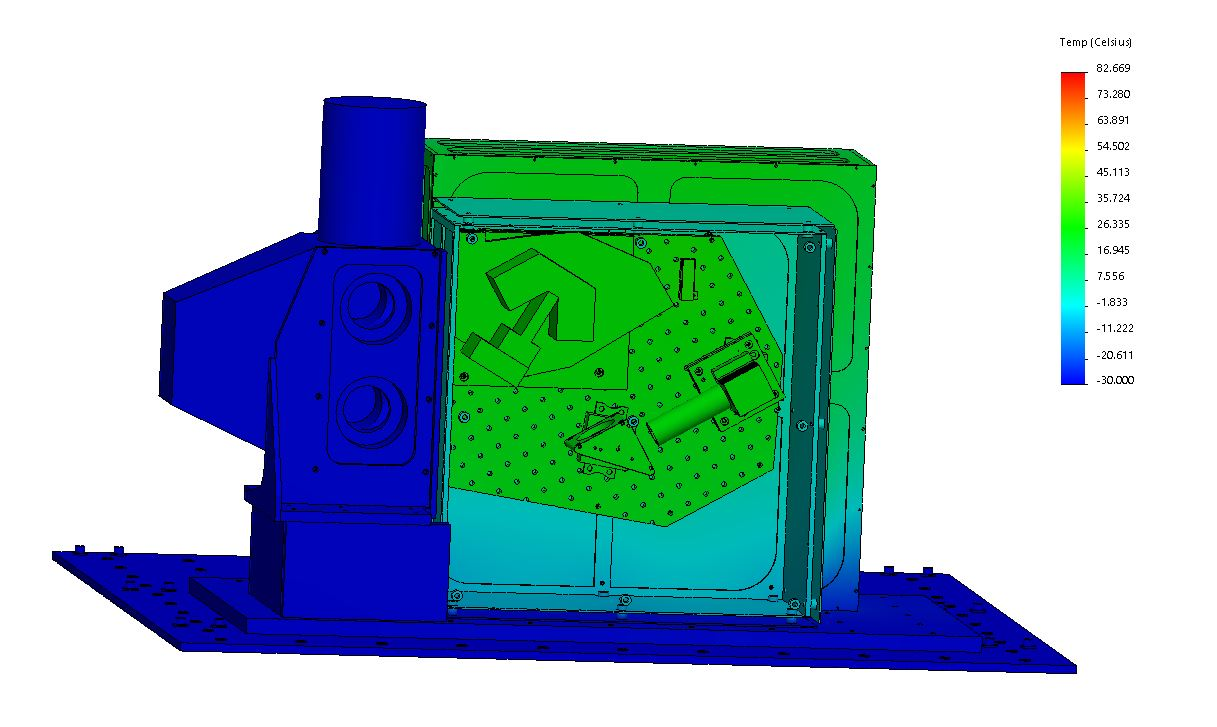
\includegraphics[width=\textwidth]{chap3_images/LIFE_V4_images/TA_Full_Model_Iter_1.JPG}
        \caption{Cold temperature case simulation for Optics Box, boxes connected.}
        \label{fig:LIFE_V4_TA_Optics_1a}
    \end{subfigure}
    \begin{subfigure}[h]{0.65\textwidth}
        \centering
        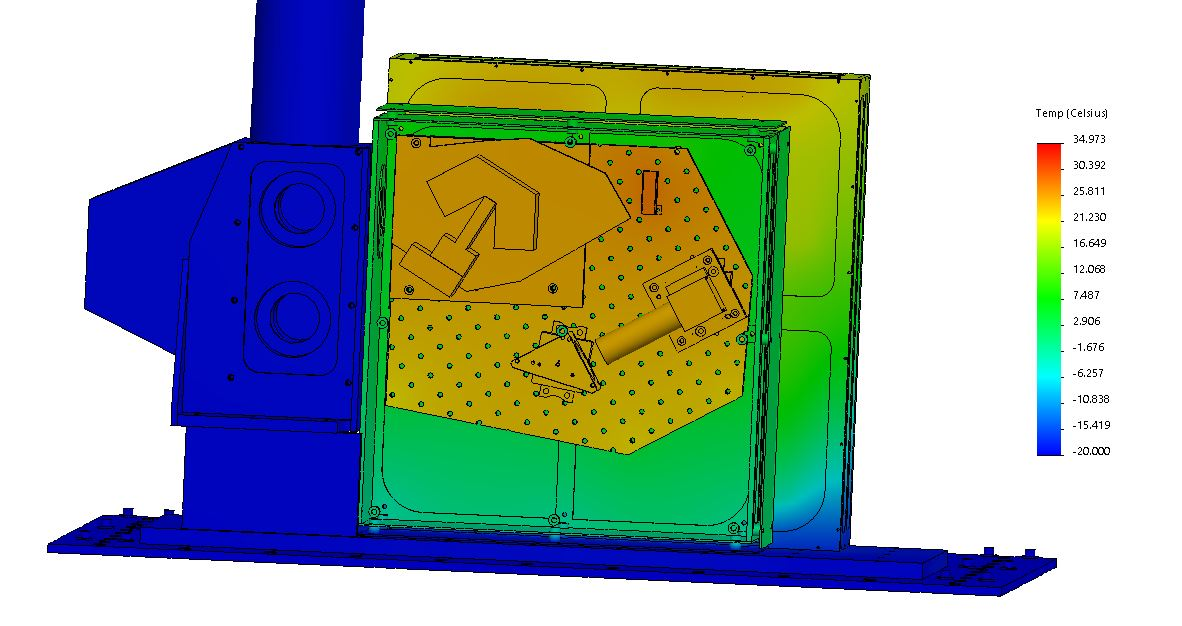
\includegraphics[width=\textwidth]{chap3_images/LIFE_V4_images/TA_Full_Model_Iter_2.JPG}
        \caption{Average temperature case simulation for Optics Box, boxes connected.}
        \label{fig:LIFE_V4_TA_Optics_1b}
    \end{subfigure}
    \begin{subfigure}[h]{0.65\textwidth}
        \centering
        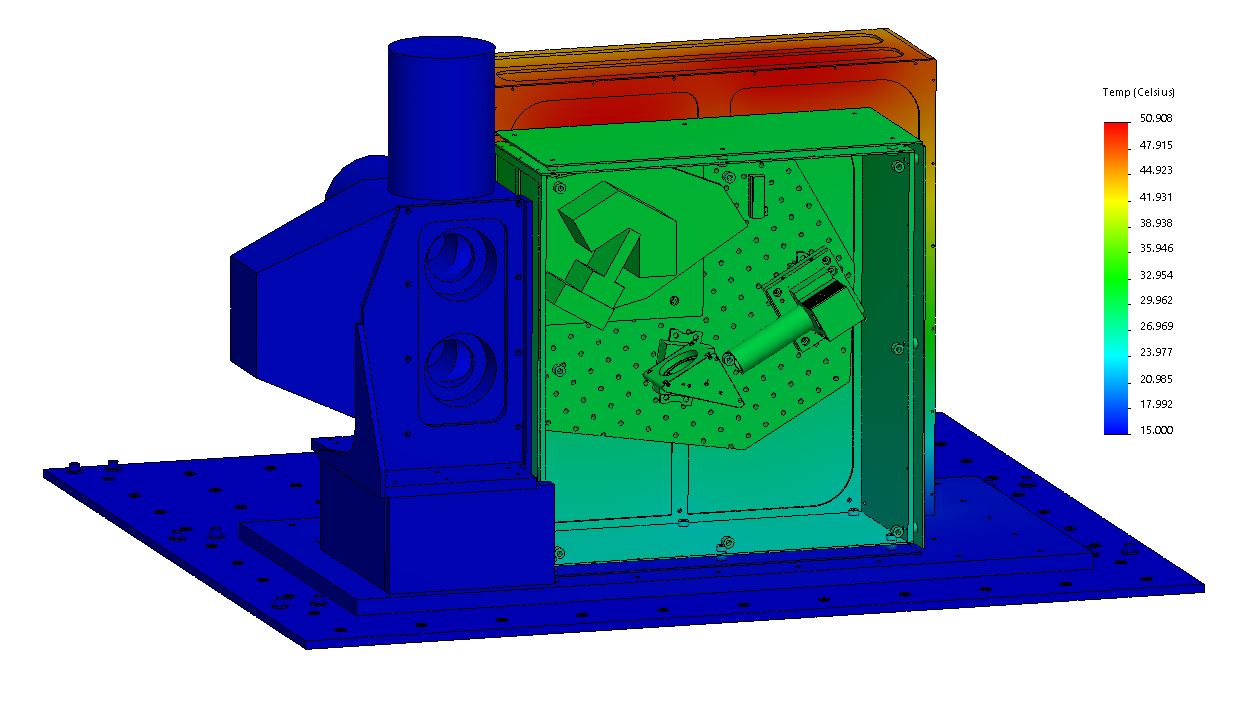
\includegraphics[width=\textwidth]{chap3_images/LIFE_V4_images/TA_Full_Model_Iter_3.JPG}
        \caption{Warm temperature case simulation for Optics Box, boxes connected.}
        \label{fig:LIFE_V4_TA_Optics_1c}
    \end{subfigure}
    \caption{Simulations for LIFE V4, Optics Box view, boxes connected.}
    \label{LIFE_V4_TA_1_Optics}
\end{figure}

\begin{figure}
    \centering
    \begin{subfigure}[h]{0.65\textwidth}
        \centering
        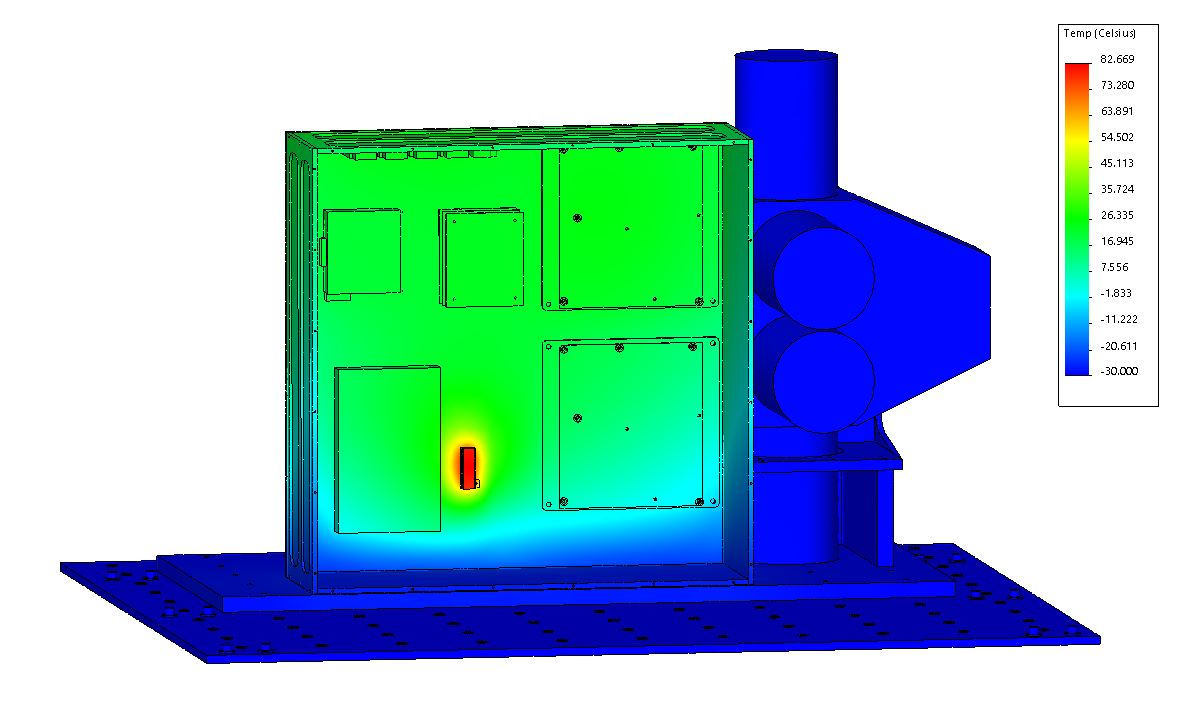
\includegraphics[width=\textwidth]{chap3_images/LIFE_V4_images/TA_Full_Model_Iter_1_ebox.JPG}
        \caption{Cold temperature case simulation for Electronics Box, boxes connected.}
        \label{fig:LIFE_V4_TA_Ebox_1a}
    \end{subfigure}
    \begin{subfigure}[h]{0.65\textwidth}
        \centering
        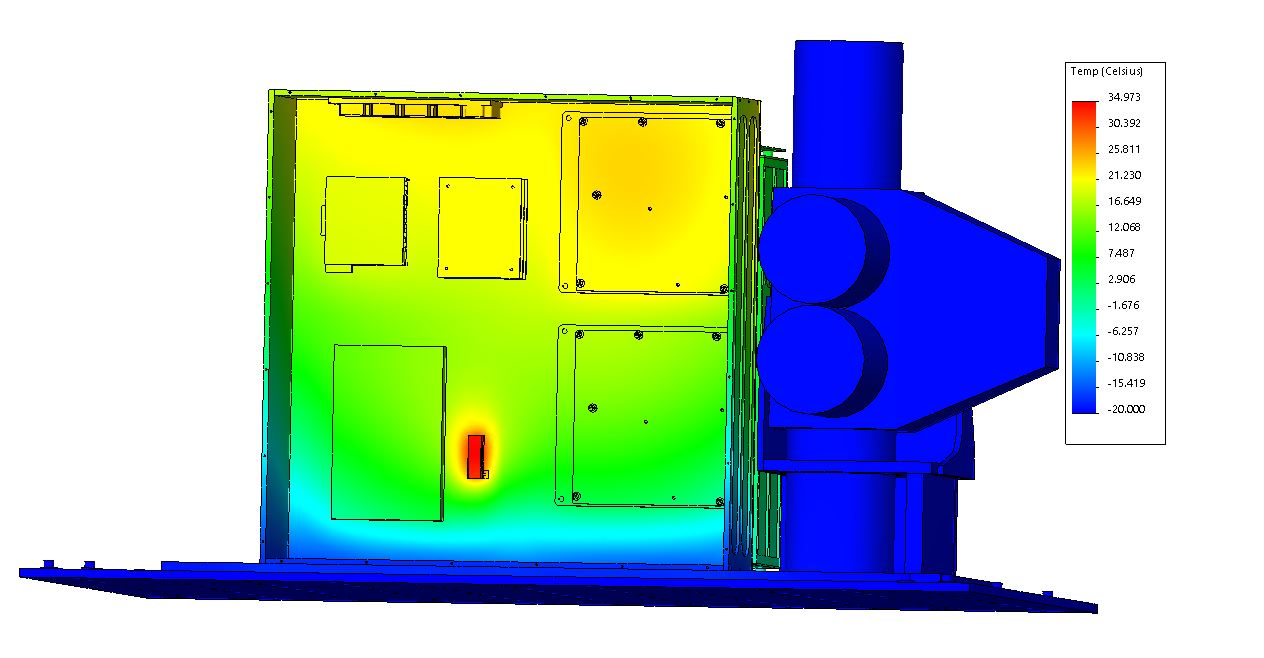
\includegraphics[width=\textwidth]{chap3_images/LIFE_V4_images/TA_Full_Model_Iter_2_ebox.JPG}
        \caption{Average temperature case simulation for Electronics Box, boxes connected.}
        \label{fig:LIFE_V4_TA_Ebox_1b}
    \end{subfigure}
    \begin{subfigure}[h]{0.65\textwidth}
        \centering
        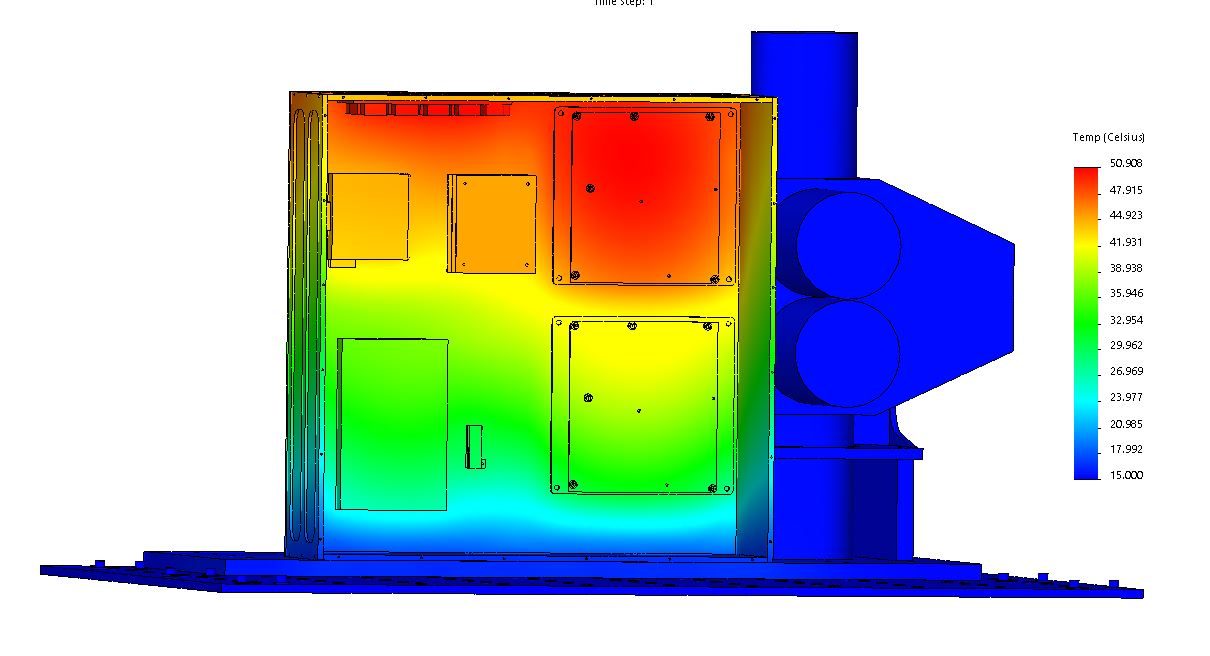
\includegraphics[width=\textwidth]{chap3_images/LIFE_V4_images/TA_Full_Model_Iter_3_ebox.JPG}
        \caption{Warm temperature case simulation for Electronics Box, boxes connected.}
        \label{fig:LIFE_V4_TA_Ebox_1c}
    \end{subfigure}
    \caption{Simulations for LIFE V4, Electronics Box view, boxes connected.}
    \label{LIFE_V4_TA_1_Ebox}
\end{figure}

Overall, the results from these simulations are positive, but show areas needing improvement. Both boxes, with the exception of part of the BMXS board, survive the cold case well, and everything is operating well in the average case. In the warm case however, the optics components and some of the electrical components are overheating. This is not as much of an issue for the Electronics Box, which will have fans to keep things cooler in the warm case (although this is still something that needs to be minimized if possible), but the Optics Box needs to be running at least 10°C cooler than these simulations show. The main reason for the high temperatures in the Optics Box is due to the connection between the outer wall and the Electronics Box wall. Although it will cause an increase in temperatures in the Electronics Box, the thermal connection between the boxes is removed, so that the optics due not exceed their required temperature limits. The design was changed to have a 5mm gap between the boxes. The same three scenarios are run as simulations, with the Optics Box heater now set as 18W, 14W, and 0W for the cold, average, and warm cases respectively, and the Electronics Box heater now set as 100W, 50W, and 0W. The results are presented in Figure \ref{LIFE_V4_TA_2_Optics} (Optics Box view) and Figure \ref{LIFE_V4_TA_2_Ebox} (Electronics Box view).

\begin{figure}
    \centering
    \begin{subfigure}[h]{0.6\textwidth}
        \centering
        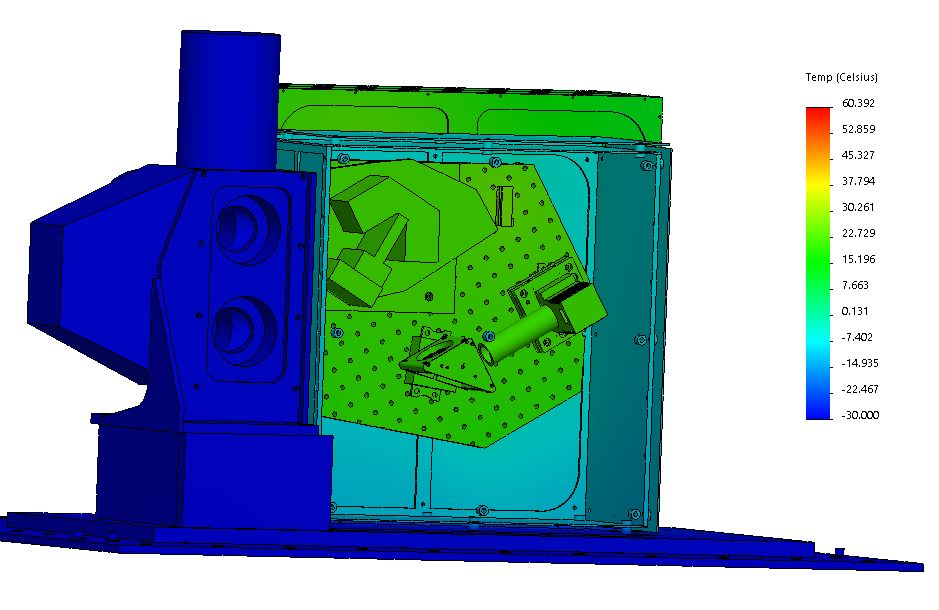
\includegraphics[width=\textwidth]{chap3_images/LIFE_V4_images/TA_Full_Model_Iter_10.JPG}
        \caption{Cold temperature case simulation for Optics Box, boxes not connected.}
        \label{fig:LIFE_V4_TA_Optics_2a}
    \end{subfigure}
    \begin{subfigure}[h]{0.6\textwidth}
        \centering
        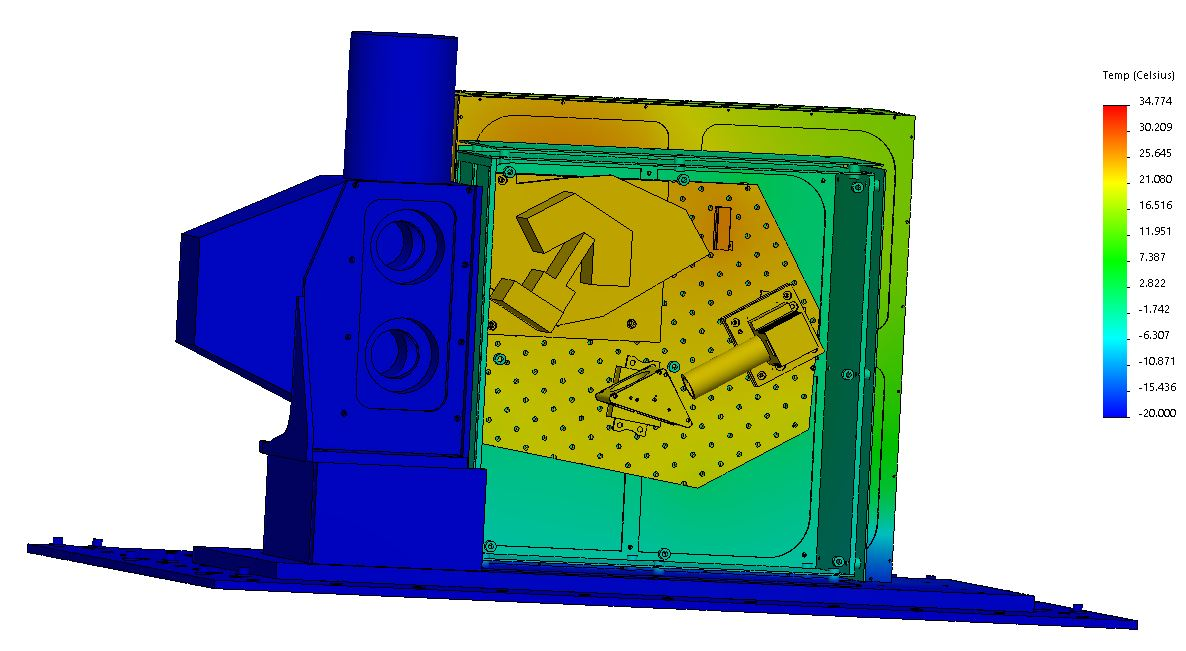
\includegraphics[width=\textwidth]{chap3_images/LIFE_V4_images/TA_Full_Model_Iter_11.JPG}
        \caption{Average temperature case simulation for Optics Box, boxes not connected.}
        \label{fig:LIFE_V4_TA_Optics_2b}
    \end{subfigure}
    \begin{subfigure}[h]{0.6\textwidth}
        \centering
        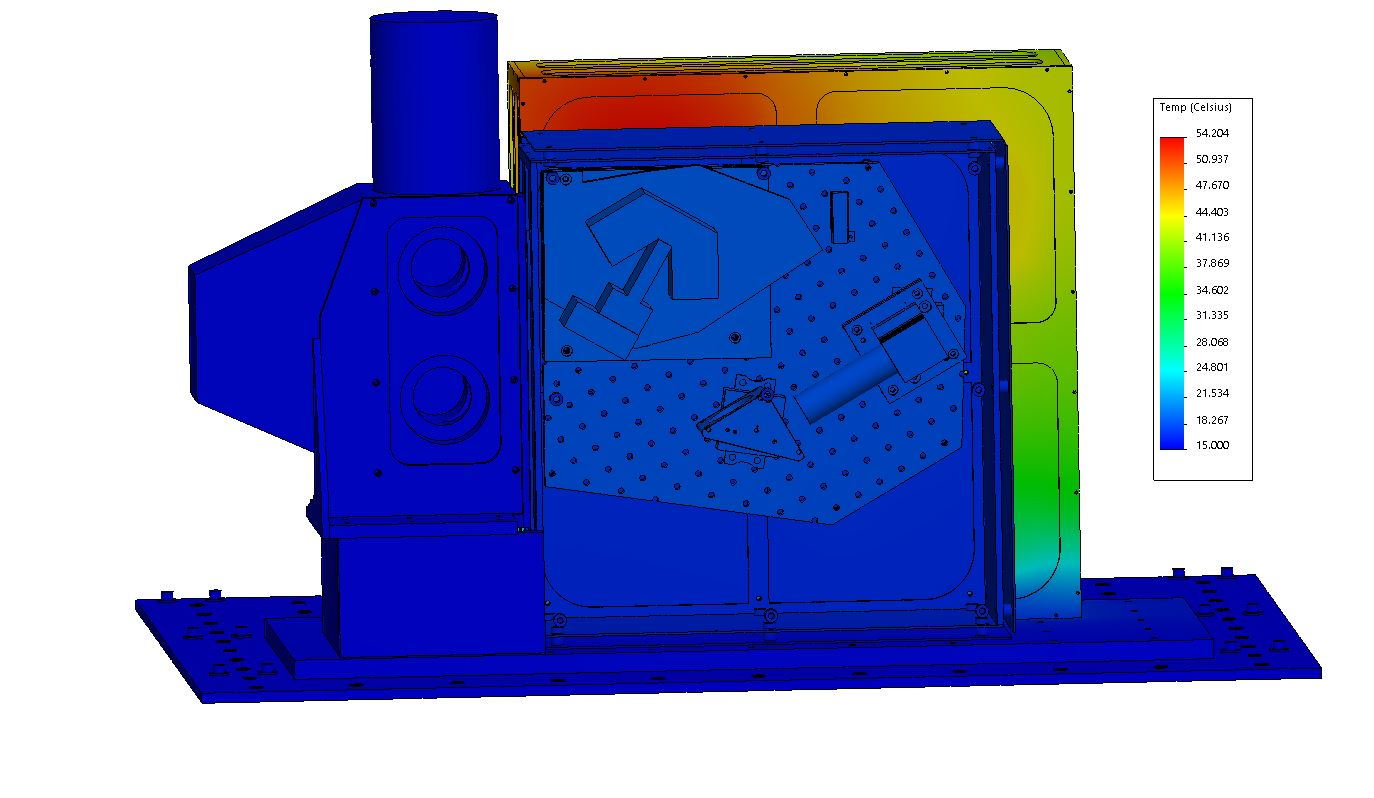
\includegraphics[width=\textwidth]{chap3_images/LIFE_V4_images/TA_Full_Model_Iter_12.JPG}
        \caption{Warm temperature case simulation for Optics Box, boxes not connected.}
        \label{fig:LIFE_V4_TA_Optics_2c}
    \end{subfigure}
    \caption{Simulations for LIFE V4, Optics Box view, with no direct thermal path between boxes.}
    \label{LIFE_V4_TA_2_Optics}
\end{figure}

\begin{figure}
    \centering
    \begin{subfigure}[h]{0.53\textwidth}
        \centering
        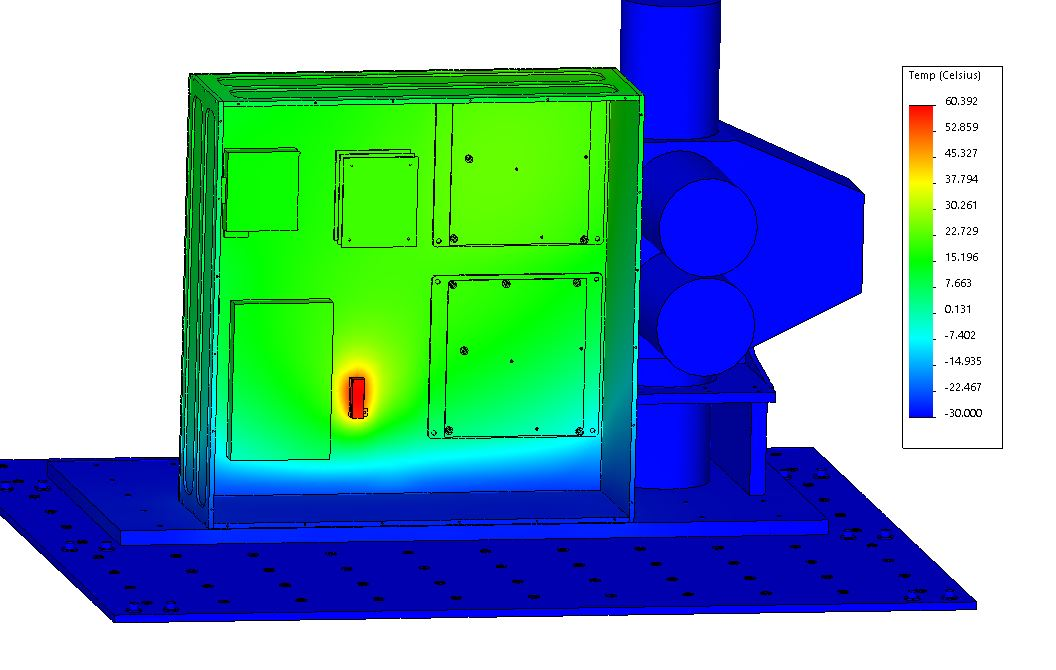
\includegraphics[width=\textwidth]{chap3_images/LIFE_V4_images/TA_Full_Model_Iter_10_ebox.JPG}
        \caption{Cold temperature case simulation for Electronics Box, boxes not connected.}
        \label{fig:LIFE_V4_TA_Ebox_2a}
    \end{subfigure}
    \begin{subfigure}[h]{0.53\textwidth}
        \centering
        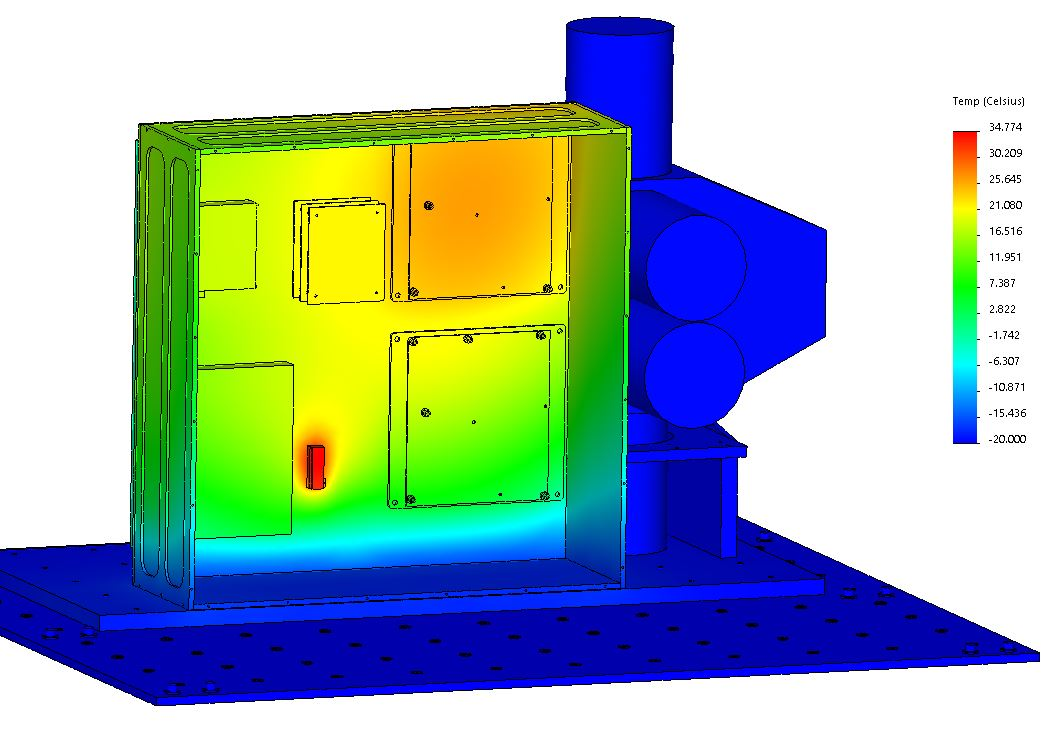
\includegraphics[width=\textwidth]{chap3_images/LIFE_V4_images/TA_Full_Model_Iter_11_ebox.JPG}
        \caption{Average temperature case simulation for Electronics Box, boxes not connected.}
        \label{fig:LIFE_V4_TA_Ebox_2b}
    \end{subfigure}
    \begin{subfigure}[h]{0.53\textwidth}
        \centering
        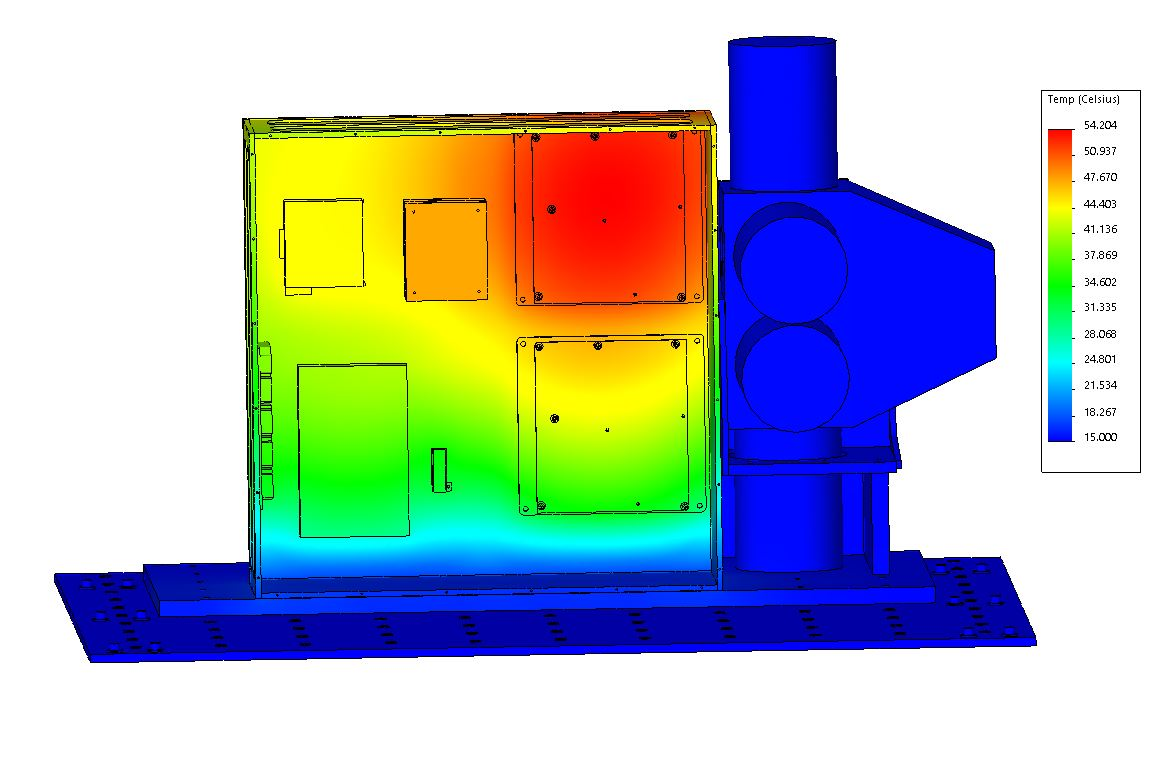
\includegraphics[width=\textwidth]{chap3_images/LIFE_V4_images/TA_Full_Model_Iter_12_ebox.JPG}
        \caption{Warm temperature case simulation for Electronics Box, boxes not connected.}
        \label{fig:LIFE_V4_TA_Ebox_2c}
    \end{subfigure}
    \caption{Simulations for LIFE V4, Electronics Box view, with no direct thermal path between boxes..}
    \label{LIFE_V4_TA_2_Ebox}
\end{figure}

With no thermal connection between the boxes, the Optics Box temperatures are now well within their required ranges. With a moderately sized heater, optical components maintain a temperature of 20°C in the cold case and warm case, and roughly 18°C in the warm case. However, with less heat being dissipated elsewhere, many components in the Electronics Box are now too warm. In the cold and average case, the components are well within their limits, and a smaller heater is required as the heat is no longer transferring the Optics Box. However, in the warm case, the DAQ board is reaching temperatures in excess of 52°C, well beyond the temperature maximum, and cooling fans may not be enough to keep it cool through continuous operation in the lab. There are also more components that will be installed in this box, which will generate more heat. A complete redesign of the electronics layout within the Electronics Box would be necessary, both for thermal reasons and space reasons. With the Optics Box requirements met for all cases, the new design only effects the Electronics Box. This leads to the third version of the electronics box, in LIFE Version 5.

\subsection{LIFE Preliminary Design: Version 5}
Towards the end of the thermal-mechanical design cycle of LIFE Version 4, the electronics design for LIFE was nearing completion. It was now known what other electronics components would need to be added: DC-DC converters (power supplies to interface with the gondola power supplies), filters for the power lines, temperature controllers, a second computer stack, and the controller for the motor within the blackbody system. After a few different iterations of the design, it was determined that there was no good way to put all electronics into one box. The box would have to be too large for the volume requirements of the gondola, or components would have to be installed very close together. This leads to difficulty in building and repair of the electrical system, and also makes meeting the thermal requirements difficult. Thus for the the next version of LIFE, Version 5, a new box would be added to the design, holding some of the instruments electrical components. The new electrical components that were placed in this box were all components necessary to operate the blackbody system, and it was thus named the \textit{Blackbody Electronics Box}. 

Outside of this addition, there were a few other changes. The Optics Box remains largely unchanged, except for the addition of smaller components such as the purge and desiccant system, which allows the box to be purged with nitrogen and kept dry before launch. The full model of LIFE V5, including this new box, is shown in Figure \ref{fig:LIFE_V5_prelim}.

\begin{figure}
    \centering
    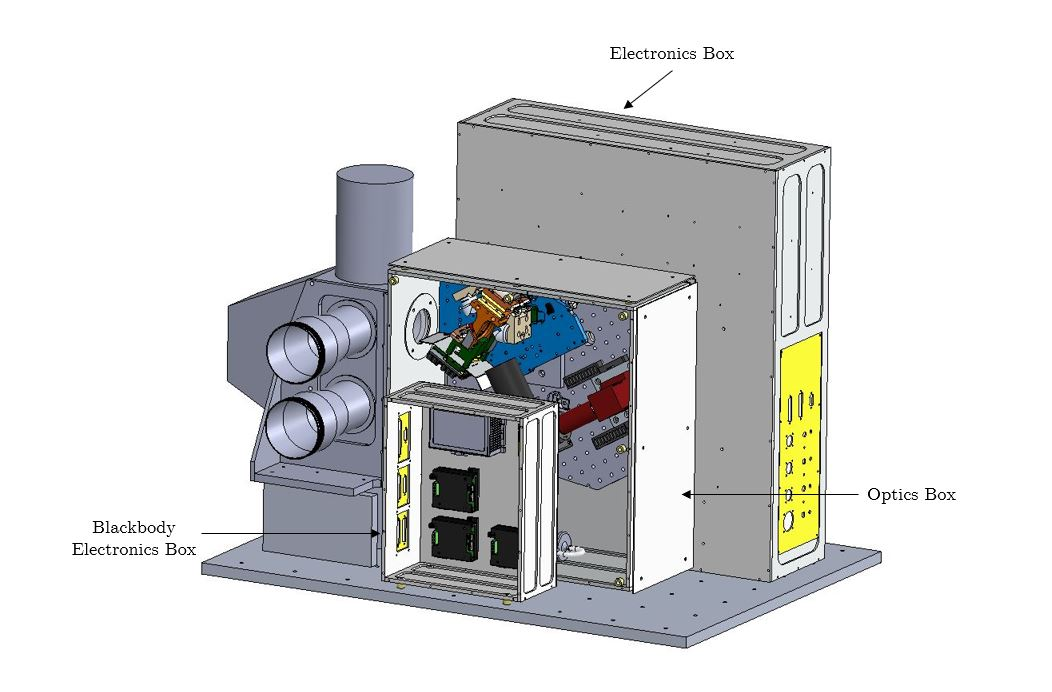
\includegraphics[width=0.7\textwidth]{chap3_images/LIFE_V5_initial_images/LIFE_V5_prelim_labelled_jpeg.JPG}
    \caption{Initial version of LIFE Version 5, with the new Blackbody Electronics Box.}
    \label{fig:LIFE_V5_prelim}
\end{figure}

\subsubsection{Electronics Box Design: Version 3}
Version 3 of the Electronics Box saw the addition of many new electronics components, which prompted a redesign of the layout. However, the main design for the layout was based upon a few requirements, from thermal simulations. The first was the location of the BMXS board. In the previous design, it was placed in the bottom right of the box, arbitrarily. As it has the most stringent minimum temperature of any component in the electronics box, it should not be placed close to the bottom of the box, which can become the coldest. As a result, it was placed hear the top of the box. The issue with placing it in this position was the potential for overheating, as it is more difficult to dissipate heat and the BMXS also has the most stringent maximum temperature, but it was less of an issue than the freezing problem. The components which had low minimum temperatures, such as the DC-DC converter, Ethernet hub, and power supply, were all placed near the base. In addition, the DC-DC converter and the power supply both dissipated a high amount of power, and placing these close to the baseplate mitigated overheating. 

In addition to the BMXS, the other parts that had a large effect on the layout were the DAQ/Pleora boards. These boards dissipated the most heat, while also having the second smallest temperature range, after the BMXS. It took many simulations to be able to place them in the correct location. First, their location was limited by their connection to the MCT Detector. Sixteen cables connect the DAQ board to the detector, and are at a finite length of less than half a meter. They had to be placed at somewhat the same height as the detector in the Optics Box to minimize distance. Beyond this constraint, the power and thermal requirements would need to be balanced for the ideal location. If the boards were too high, they would not be able to dissipate enough heat in the hot case, and would overheat. However, if they were placed too low, they would freeze in the cold case if the Pleora board attachments fell below 0°C. These boards were moved up and down and placed in various orientations through many thermal simulation iterations until they would be able to meet the minimum temperature requirements in the cold case and the maximum temperature requirements in the hot case. The final location for these boards had only 5mm of error in moving up and down to continue staying within the required range. The heaters used and the resulting temperatures are described in the thermal section. Beyond these boards, the remaining components of temperature controllers and computer stacks could be placed somewhat freely, as they had wide temperature ranges and had relatively low heat dissipation. The result of these layout iterations and thermal simulations is Version 3 of the Electronics Box, shown in Figure \ref{fig:EBOX_V3}.

\begin{figure}
    \centering
    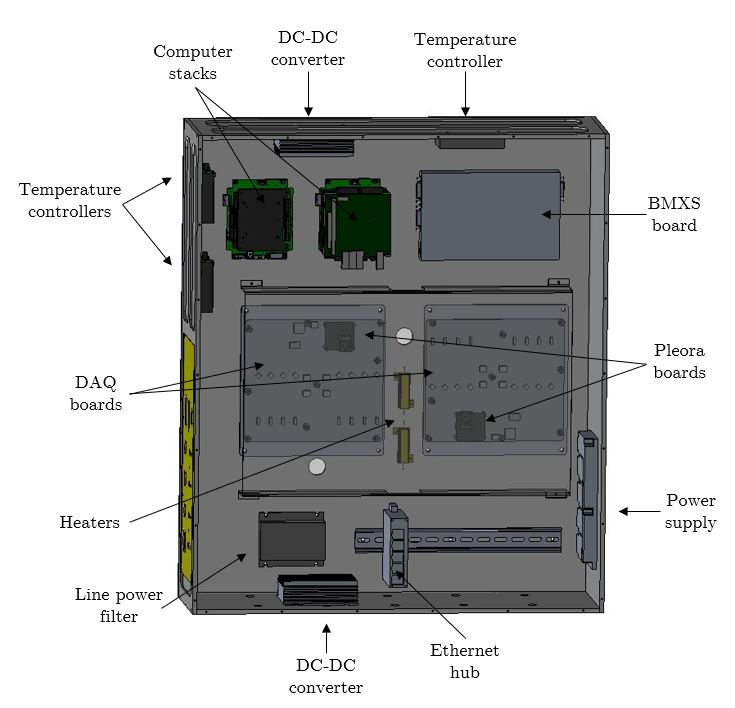
\includegraphics[width=\textwidth]{chap3_images/LIFE_V5_initial_images/Ebox_V3_init_labelled.JPG}
    \caption{Electronics Box Version 3, with more components added.}
    \label{fig:EBOX_V3}
\end{figure}

Another addition to this box beyond Version 2 was the first version of the breakout board, or the wall through where external connections would be made. This was designed using a third party software outside SolidWorks and ordered independently, outside of the machine shops. There was also planned to be a protective cover placed over the DAQ boards as they were the most electro-static discharge (ESD) sensitive components in the instrument, to stop any accidental contact with these boards during construction or repair. However it was decided later during the build that the implementation was not necessary. 

\subsubsection{Blackbody Electronics Box Design: Version 1}
This box housed components that were required to operate the blackbody system, and could not fit within the main Electronics Box while meeting size and space requirements. The core components of the new box are three temperature controllers and a motor controller. Two of the three temperature controllers control the blackbody temperatures, the third would control the temperature of this new box, and the motor controller is for the blackbody system. While less thermally sensitive than the other boxes, the thermal design of this box was still important due to the temperature range of the motor controller. As described in the thermal section, a heater was added to this box for the purpose of keeping the temperature of the box above 0°C. A few more components would be added later, but these were most important for the thermal design. A model of this box is shown in Figure \ref{fig:BBEBOX_PRELIM}.

\begin{figure}
    \centering
    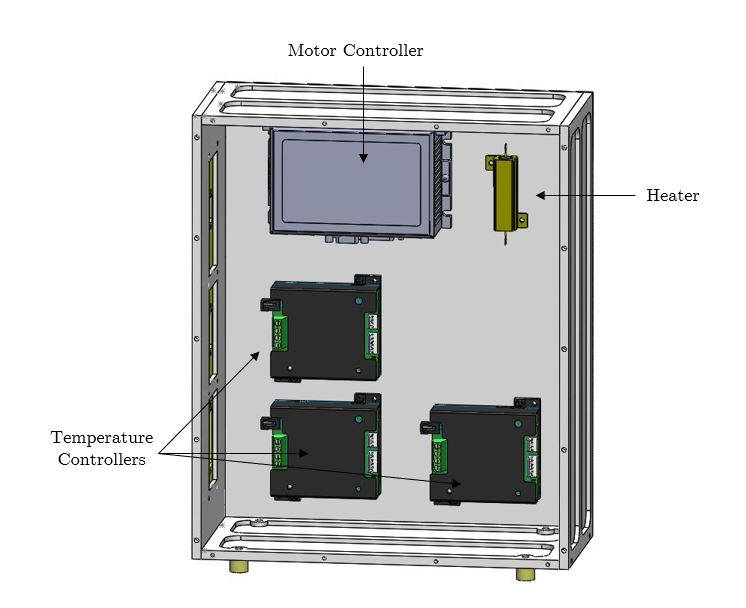
\includegraphics[width=0.8\textwidth]{chap3_images/LIFE_V5_initial_images/BBEbox_V1_init_labelled.JPG}
    \caption{Initial model of the Blackbody Electronics Box, which contains components which control the blackbodies.}
    \label{fig:BBEBOX_PRELIM}
\end{figure}

\subsubsection{LIFE Version 5: Thermal Analysis}
As with previous analyses, the simulations were split into the three major scenarios: The cold case, average case, and warm case. As the thermal design of the Optics Box from the previous thermal analysis met requirements, this will mainly focus on the Electronics Box and Blackbody Electronics Box. Numerous iterations were done with different heater values, heater locations, and electronics locations to ensure that the most critical components would meet requirements. The Electronics Box heater was split in two, becoming two resistors wired in parallel, which would aid in redundancy should one of them fail during flight. Spreading them out also means a better heat distribution to delicate components, and requires smaller heaters. For the cold case, the thermal simulation inputs were as follows: the minimum temperature was lowered to -40°C, to better simulate what could be experienced during the ascent, even for a short period of time. The heaters in the electronics box dissipated 60W each, the optics heater dissipated 22W, and the Blackbody Electronics Box heater dissipated 60W. The model for the simulation is shown in Figure \ref{LIFE_V5_Prelim_TA_COLD}.

\begin{figure}
    \centering
    \begin{subfigure}[h]{0.9\textwidth}
        \centering
        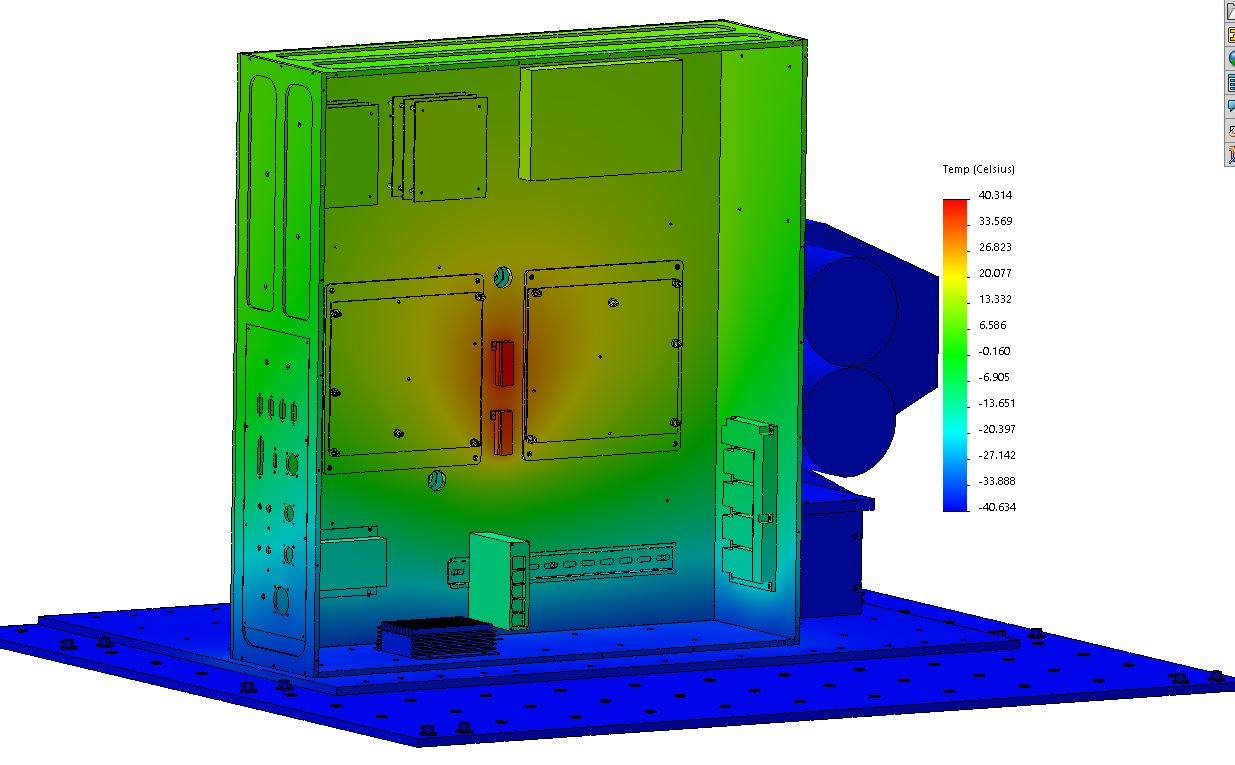
\includegraphics[width=\textwidth]{chap3_images/LIFE_V5_initial_images/Iteration_1_ebox_no_labels.JPG}
        \caption{Cold temperature case simulation for LIFE V5, Electronics Box view.}
        \label{fig:LIFE_V5_TA_COLD_EBOX}
    \end{subfigure}
    \begin{subfigure}[h]{0.9\textwidth}
        \centering
        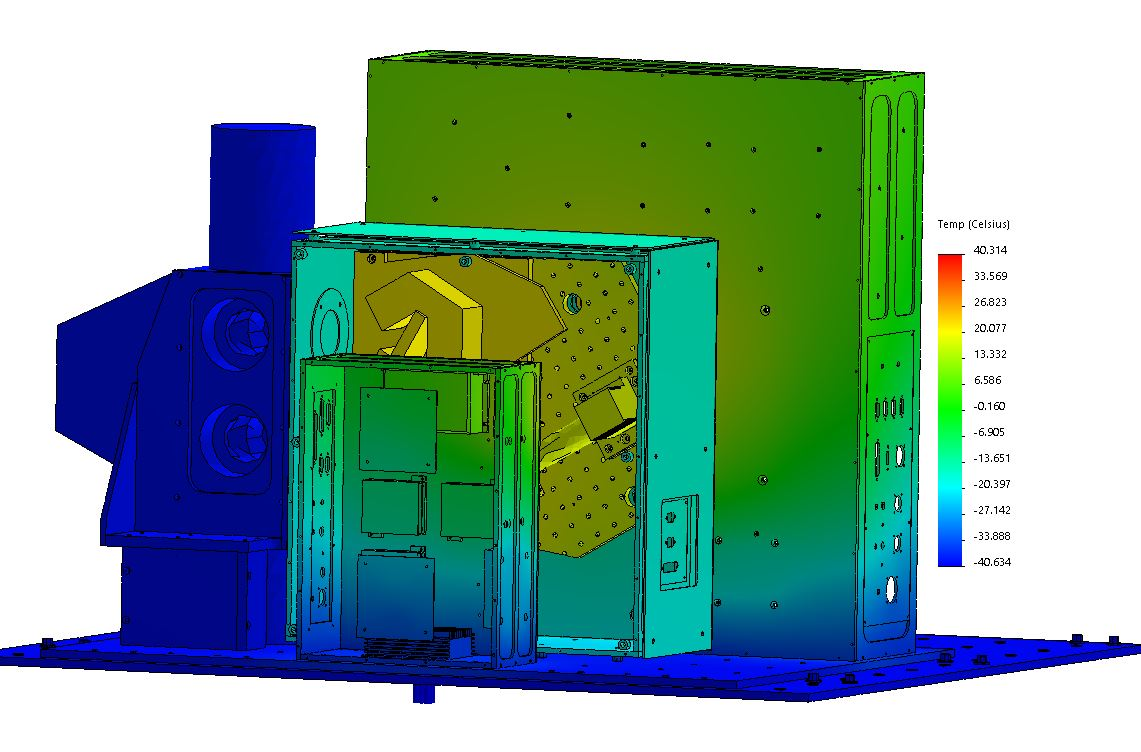
\includegraphics[width=\textwidth]{chap3_images/LIFE_V5_initial_images/Iteration_1_no_labels.JPG}
        \caption{Cold temperature case simulation for LIFE V5, Optics Box view.}
        \label{fig:LIFE_V4_TA_COLD_OBOX}
    \end{subfigure}
    \caption{Front and rear view of LIFE V5 cold scenario simulation.}
    \label{LIFE_V5_Prelim_TA_COLD}
\end{figure}

\begin{figure}
    \centering
    \begin{subfigure}[h]{0.9\textwidth}
        \centering
        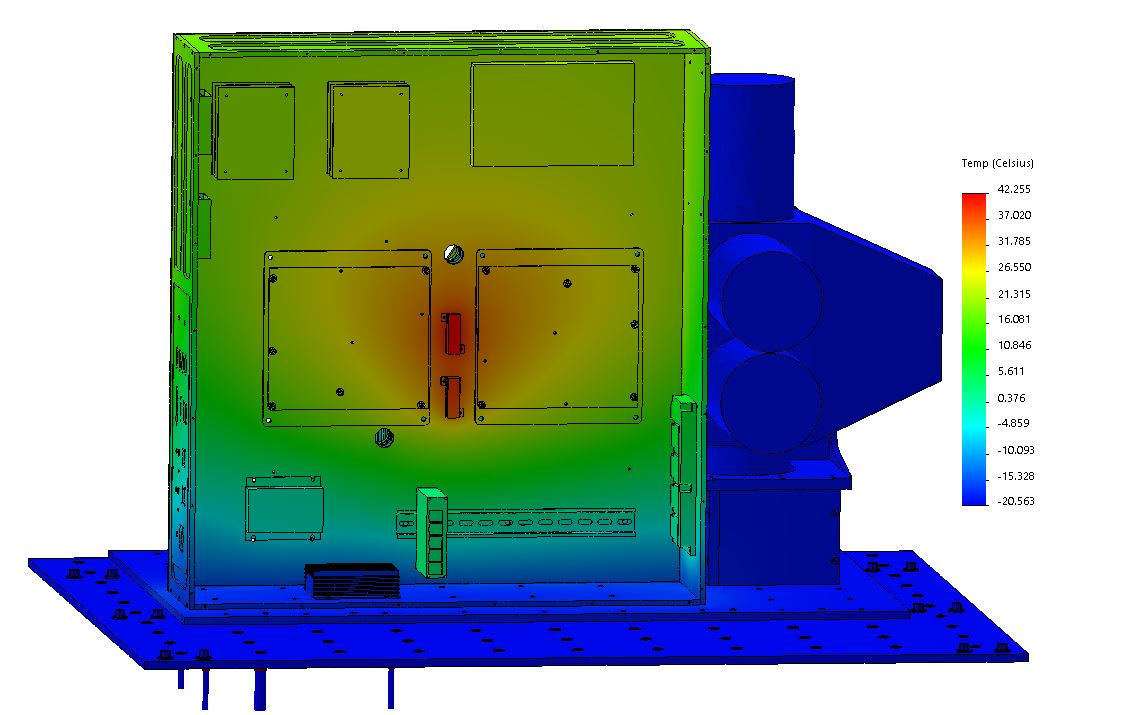
\includegraphics[width=\textwidth]{chap3_images/LIFE_V5_initial_images/Iteration_2_ebox_no_labels.JPG}
        \caption{Average temperature case simulation for LIFE V5, Electronics Box view.}
        \label{fig:LIFE_V5_TA_AVG_EBOX}
    \end{subfigure}
    \begin{subfigure}[h]{0.9\textwidth}
        \centering
        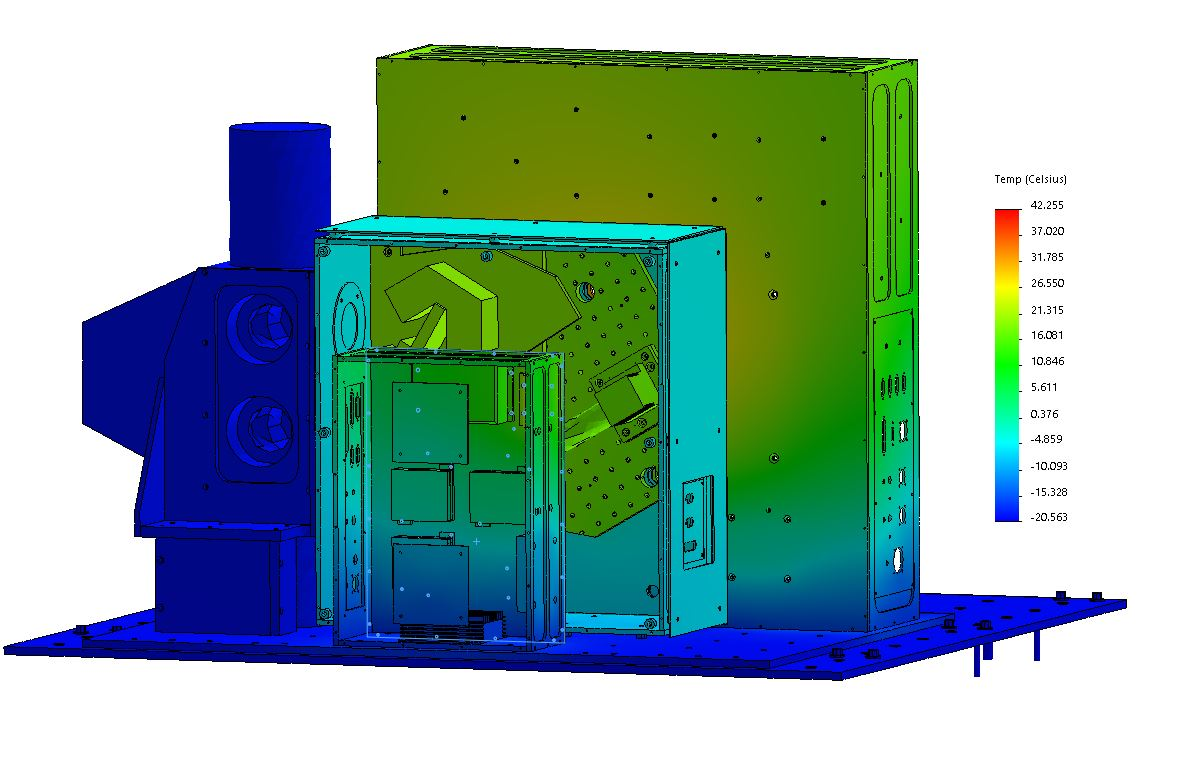
\includegraphics[width=\textwidth]{chap3_images/LIFE_V5_initial_images/Iteration_2_no_labels.JPG}
        \caption{Average temperature case simulation for LIFE V5, Optics Box view.}
        \label{fig:LIFE_V4_TA_AVG_OBOX}
    \end{subfigure}
    \caption{Front and rear view of LIFE V5 average scenario simulation.}
    \label{LIFE_V5_Prelim_TA_AVG}
\end{figure}

\begin{figure}
    \centering
    \begin{subfigure}[h]{0.9\textwidth}
        \centering
        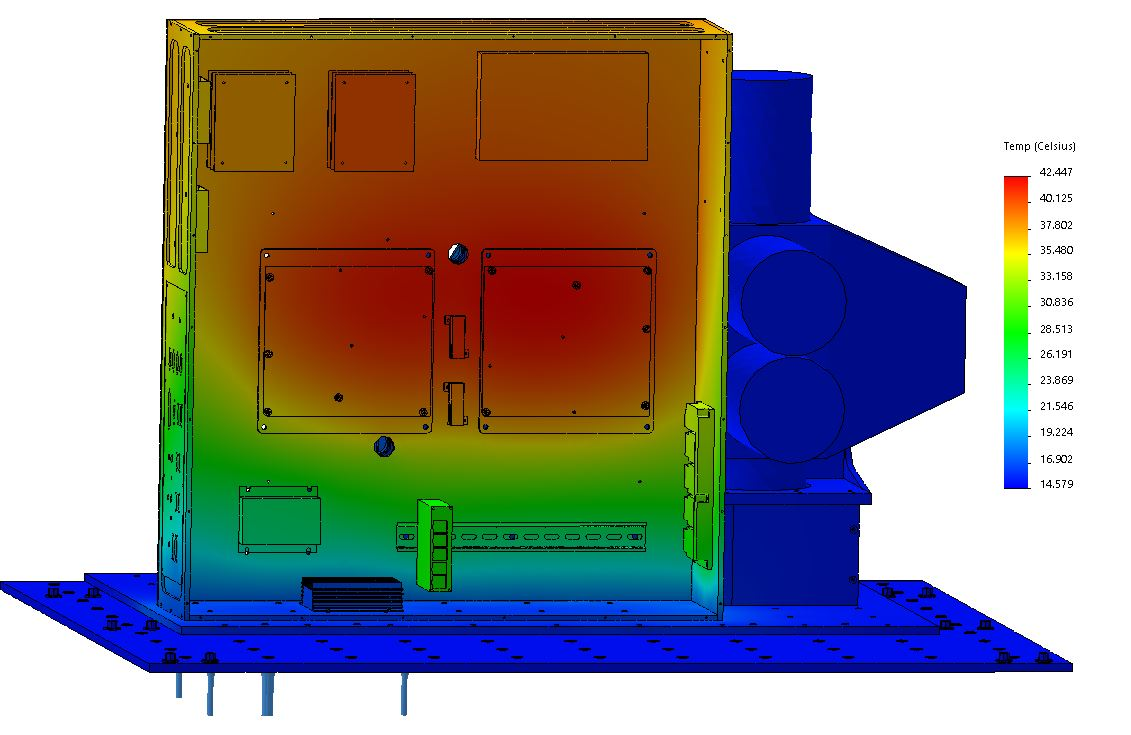
\includegraphics[width=\textwidth]{chap3_images/LIFE_V5_initial_images/Iteration_3_ebox_no_labels.JPG}
        \caption{Warm temperature case simulation for LIFE V5, Electronics Box view.}
        \label{fig:LIFE_V5_TA_WARM_EBOX}
    \end{subfigure}
    \begin{subfigure}[h]{0.9\textwidth}
        \centering
        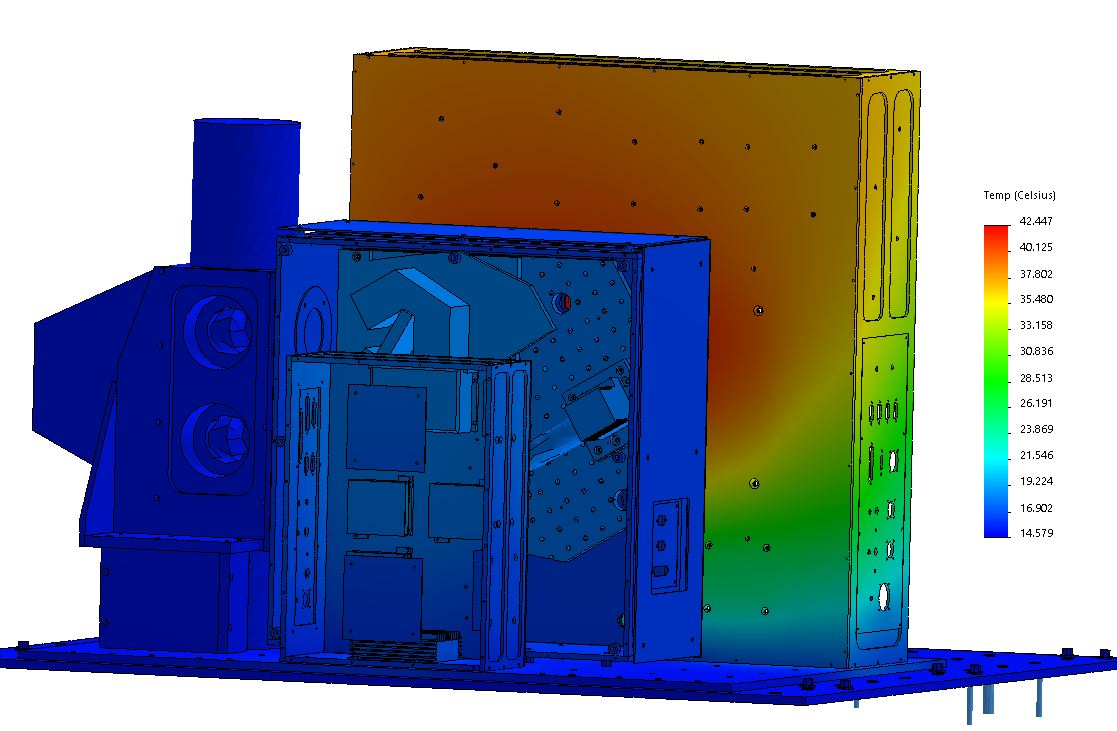
\includegraphics[width=\textwidth]{chap3_images/LIFE_V5_initial_images/Iteration_3_no_labels.JPG}
        \caption{Warm temperature case simulation for LIFE V5, Optics Box view.}
        \label{fig:LIFE_V4_TA_WARM_OBOX}
    \end{subfigure}
    \caption{Front and rear view of LIFE V5 warm scenario simulation.}
    \label{LIFE_V5_Prelim_TA_WARM}
\end{figure}

The component temperatures meet the required temperature ranges. Although the DAQ boards drop below 0°C in some areas, the locations where the Pleora boards are attached stay above 0°C, as required. For the average case, the inputs were as follows: the baseplate temperature set as -20°C, the electronics box heaters dissipate 40W each, the Optics Box heater dissipates 14W, and the Blackbody Electronics Box heater dissipates 40W. The model for the average temperature scenario is shown in Figure \ref{LIFE_V5_Prelim_TA_AVG}.

The temperature requirements are met for the average temperature case. Finally, examining the warm case, it must be ensured that the Electronics Box, and specifically the BMXS board, will not overheat. For this final case, the baseplate temperature set as 15°C, and all heaters are off. The model for the warm (lab) temperature scenario is shown in Figure \ref{LIFE_V5_Prelim_TA_WARM}.

Here, the Electronics Box is close to overheating, but manages to stay within the required temperature range. Ideally, there is a margin of error from the simulation to the requirements, but this is the worst case scenario. This simulation assumes all electronics on full power, for an indefinite amount of time, with no fans. Most important will be the installation of fans, which will run while the instrument is in the lab, ensuring the components do not overheat. So, overall, this design meets all thermal requirements, and a final, detailed design can be created. However, one more version of LIFE was created, as an alternate to Version 5. It is described in the subsequent section.

\subsection{LIFE Preliminary Design: Version 6}
One issue with LIFE Version 5 is that although some components were moved to a separate Electronics Box, the main box still contains many components. Most importantly, it contains the electronics for the Optics Box system: the BMXS board, the DAQ board, and their power supply. The BMXS board and DAQ board are both highly ESD-sensitive components, and must be handled very carefully. Less time spent working around these components means a lower chance that they could be touched accidentally while working, causing potential damage to these components. An idea was raised of moving all non-optics related electrical components into their own box, leaving all the components necessary for the operation of the optical system in their own box. This would lower time spent working around sensitive components and lowering the chance of unintended damage to the electronics. The Optics Box would remain the same. This new design was named LIFE Version 6, and a model is shown in Figure \ref{fig:LIFE_V6}.

\begin{figure}
    \centering
    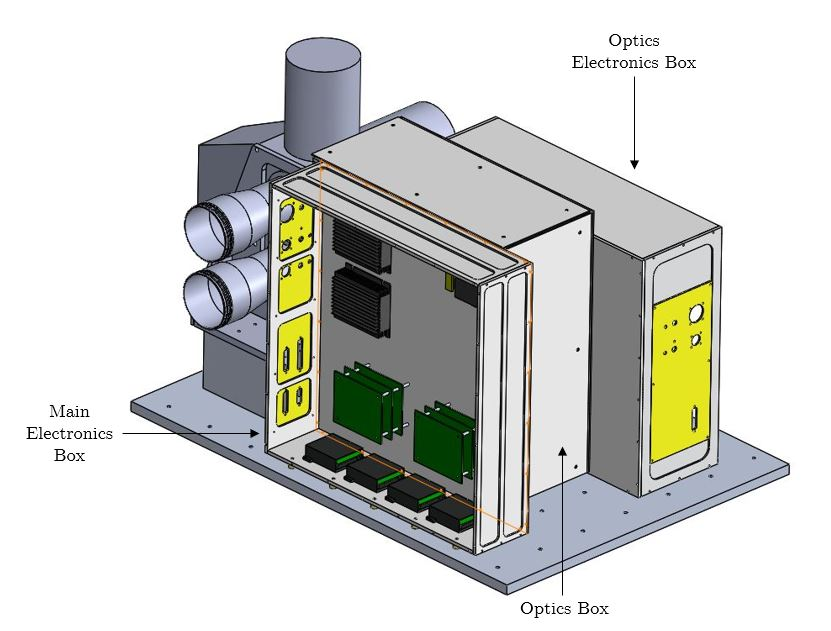
\includegraphics[width=0.7\textwidth]{chap3_images/LIFE_V6_images/LIFE_V6_img2_labelled.JPG}
    \caption{LIFE Version 6, which shifted components between electronics boxes to better protect the optics electronics.}
    \label{fig:LIFE_V6}
\end{figure}

The box that would contain all Electronics for the Optical System was named the \textit{Optics-Electronics Box}. It housed the two DAQ boards with the Pleora boards, the Ethernet hub, BMXS board, power supply, heaters for for the DAQ boards and BMXS, and their associated temperature controllers. The connections to the Electronics Box would be for power to the temperature controllers and heaters, and the Ethernet connection from the Ethernet hub to the computer stack. A model of this is shown in Figure \ref{fig:OPTOEBOX_V1}. The electronics box, holding the rest of the components, is shown in Figure \ref{fig:EBOX_V4}.

\begin{figure}
    \centering
    \includegraphics[width=0.6\textwidth]{chap3_images/LIFE_V6_images/optoebox_V1.JPG}
    \caption{A new box, meant to replace the Blackbody Electronics Box, which houses only the optics electronics.}
    \label{fig:OPTOEBOX_V1}
\end{figure}

\begin{figure}
    \centering
    \includegraphics[width=0.6\textwidth]{chap3_images/LIFE_V6_images/EBOX_V4.JPG}
    \caption{The fourth version of the Electronics Box, which here houses all electronics except the optical system components.}
    \label{fig:EBOX_V4}
\end{figure}

An issue with this design is that the BMXS board now needs to be placed on the base, where the temperature changes can be much larger. This is why in Version 5 it was placed above the DAQ boards. The DAQ boards cannot be moved lower, as they would freeze if they were too close to the base as well. One option to improve the thermal characteristics would be to add more heaters around the BMXS board, but the instrument is already drawing a large amount of heater power, approaching the limit of what can be supplied by the gondola. The other option would be to move the BMXS board above the DAQ boards, however this would make the box almost as large as before, adding weight, which is also almost at the required limit.

The were no detailed thermal analysis done for this design. After redesigning, it was determined that it was not worth the time to perform many new thermal iterations and to redesign the connections between boxes and components, which had already been designed to a large extent for the previous design. The solution for the original problem, the ESD-sensitive components, was to place a cover over them, as discussed previously (this was added after Version 6, but was still part of the Version 5 design). Thus this new design was scrapped, and the final design chosen was Version 5. The next section goes into the detailed design of this model.

\subsection{Final LIFE Design: Version 5 Revisited}
The design chosen to go ahead with the detailed design was Version 5. The detailed design includes a number of changes to the mechanical design, such as adding components that are not necessary to the thermal model. These components include connectors and fasteners, cables, and components that were omitted from thermal designs due to their complex shapes, including detailed board models. The blackbody design is also changed to show alterations made specifically for its use in the LIFE instrument. The final LIFE design also includes a more detailed thermal analysis, including radiation and other factors, which will have effects on characteristics such as the material coating. When the detailed design is complete, the model can be sent to be manufactured.

\subsubsection{Final Thermal Simulations}

The thermal analysis was re-examined in more detail first. A notable exception to the previous thermal analyses was the exclusion of radiation. Through some initial tests, it was found that radiation would have a small effect on the final thermal model. It also exponentially increased the simulation solving time, and as iterations needed to happen quickly in the initial designs, it was ignored. As this is now the final design, it was included in the analysis. The initial assumption was correct, in that for a typical bare aluminum surface, the emissivity is very low, at roughly 0.1. Adding radiation to the design cooled components slightly, but a negligible amount. However, bare aluminum is not a good surface, especially for high altitude balloon applications, due to rust. Typically, the boxes are painted or anodized to mitigate this.

Both painting and anodizing have a large effect on radiation. Painting, depending on the color and type of paint used, can increase emissivity to as much as 0.9. Anodization typically increases emissivity of aluminum to 0.77. This would dramatically reduce temperatures, especially in the Electronics Box, where temperatures are high. The box would get much too cold with an emissivity of 0.9, with some temperatures reaching 20°C below their recommended temperature ranges. The only option was to use anodization, and to improve heating. The Blackbody Electronics Box and Optics Box remained in good temperature ranges even with anodization, so the only changes needed to be made were in the Electronics Box. This was done by changing the number of heaters from two to four, and moving them to locations as close as possible to delicate components, specifically the Pleora Boards and the BMXS board. Two heaters were placed close to the Pleora Board on the right side, which was closest to the bottom of the box. This would help counteract the cold temperature that resulted from being closer to the gondola deck. Another heater was placed close to the other Pleora board, which as it is higher did not get as cold. The final heater was placed next to the BMXS board. This is not shown in the following temperature simulations, as this change was made just prior to construction.

A final change made to the thermal design was the addition of a garolite spacer between the Optics Box and Blackbody system. To ensure the stability of the Optics Box during flight (as it was sitting on spacers and therefore not as sturdy as the other boxes), the Optics Box was to be bolted directly to the Blackbody system. This would help with stability as well as help align the optical path between the two systems. However, a metal spacer could not be used as that would introduce a new thermal path to the Optics Box. To ensure thermal insulation, a spacer was machined out of garolite, an epoxy material which has good thermal insulation properties while also having low off-gassing properties.

With these changes to the surface coating and the addition of the garolite spacer, another set of thermal simulations were completed. This consisted of radiation on all box surfaces, with an emissivity value of 0.77, and 30W for each heater in the Electronics Box, 55W for the heater in the Blackbody Electronics Box, and 22W for the heater in the Optics Box. The resulting simulations are given in Figures \ref{LIFE_V5_FINAL_TA_COLD}, \ref{LIFE_V5_FINAL_TA_AVG}, and \ref{LIFE_V5_FINAL_TA_WARM} for the cold, average, and warm scenarios respectively. 

\begin{figure}
    \centering
    \begin{subfigure}[h]{0.9\textwidth}
        \centering
        \includegraphics[width=\textwidth]{chap3_images/LIFE_V5_initial_images/Iteration_1_ebox_no_labels.JPG}
        \caption{Cold temperature case simulation for final LIFE model, Electronics Box view.}
        \label{fig:LIFE_V5_FINAL_TA_COLD_EBOX}
    \end{subfigure}
    \begin{subfigure}[h]{0.9\textwidth}
        \centering
        \includegraphics[width=\textwidth]{chap3_images/LIFE_V5_initial_images/Iteration_1_no_labels.JPG}
        \caption{Cold temperature case simulation for final LIFE model, Optics Box view.}
        \label{fig:LIFE_V5_FINAL_TA_COLD_OBOX}
    \end{subfigure}
    \caption{Front and rear view of the final LIFE model cold scenario simulation.}
    \label{LIFE_V5_FINAL_TA_COLD}
\end{figure}

\begin{figure}
    \centering
    \begin{subfigure}[h]{0.9\textwidth}
        \centering
        \includegraphics[width=\textwidth]{chap3_images/LIFE_V5_initial_images/Iteration_2_ebox_no_labels.JPG}
        \caption{Average temperature case simulation for final LIFE model, Electronics Box view.}
        \label{fig:LIFE_V5_FINAL_TA_AVG_EBOX}
    \end{subfigure}
    \begin{subfigure}[h]{0.9\textwidth}
        \centering
        \includegraphics[width=\textwidth]{chap3_images/LIFE_V5_initial_images/Iteration_2_no_labels.JPG}
        \caption{Average temperature case simulation for final LIFE model, Optics Box view.}
        \label{fig:LIFE_V5_FINAL_TA_AVG_OBOX}
    \end{subfigure}
    \caption{Front and rear view of the final LIFE model average scenario simulation.}
    \label{LIFE_V5_FINAL_TA_AVG}
\end{figure}

\begin{figure}
    \centering
    \begin{subfigure}[h]{0.9\textwidth}
        \centering
        \includegraphics[width=\textwidth]{chap3_images/LIFE_V5_initial_images/Iteration_3_ebox_no_labels.JPG}
        \caption{Warm temperature case simulation for final LIFE model, Electronics Box view.}
        \label{fig:LIFE_V5_FINAL_TA_WARM_EBOX}
    \end{subfigure}
    \begin{subfigure}[h]{0.9\textwidth}
        \centering
        \includegraphics[width=\textwidth]{chap3_images/LIFE_V5_initial_images/Iteration_3_no_labels.JPG}
        \caption{Warm temperature case simulation for final LIFE model, Optics Box view.}
        \label{fig:LIFE_V5_FINAL_TA_WARM_OBOX}
    \end{subfigure}
    \caption{Front and rear view of the final LIFE model warm scenario simulation.}
    \label{LIFE_V5_FINAL_TA_WARM}
\end{figure}

These simulations show that with the anodization, all components fall within their temperature limits. The closest components are the Pleora boards, but the heaters are well placed to heat them even if the rest of the DAQ board falls below 0°C. The only part of these board that must be above 0°C are where the Pleora boards are connected, as the DAQ board minimum temperature is much lower at -40°C. The final choice to be made was what color anodization should be chosen. Ideally, white would be the best choice, to lower the absorptivity, so in the case that the instrument did see the sun it would not be highly affected. However, white is not an option for anodization as a result of the manufacturing process. The next lightest options were a clear anodization coat, or a gold anodization. Gold was chosen for its high reflectivity, lowering the absorptivity if it sees the sun. This was the final change made to the thermal model before manufacturing, although as described later, a few fixes were needed following the results of the TVAC tests to align the model with what was seen during tests.

\subsubsection{Final Mechanical Changes \& Models}\label{Mech_changes}
Another part of the design that is updated is the Blackbody system. The bottom hot and warm blackbodies are removed, as they are not useful to the instrument in the LIFE flight configuration, and are heavy. Also removed are the viewport baffles. These are taken off because the instrument needs to view downwards at a slight angle of 2.86°. This is done by tilting the mirror downwards, rather than tilting the optical system or the optics box, which was deemed too difficult. With the mirror tilted downwards the FOV may clip the edge of the baffle, so to ensure a full FOV it is removed. It is also noted that the cold blackbody will not be used during flight, so the electronics to control and operate this blackbody are not present in the instrument; it is connected to an external system in the lab for operation.

A number of mechanical changes are made. First, fasteners are added to the model. This includes all bolts, washers, nuts, and spacers needed to connect boxes together and to fasten electronics. This is done to ensure that all holes are in the correct location in regards to other parts or the connection locations of the electronics, so that everything fits together as expected after manufacturing. The next step of the design was to add connectors and cables to the electronics design. The connectors were to ensure that the holes on the breakout boards were the correct size, and that there was enough room to make connections; if the connector of a component was too long it may overlap with a nearby component, which would need to be accounted for. Also added in conjunction with this were models of the cables and wires, using the SolidWorks Routing tool. This allowed cable lengths to be determined in the model, to ensure that no wires are wasted and to ensure clean and efficient cable routing inside the boxes, keeping them out of the way of any sensitive components.

The final model of the LIFE instrument before construction is shown in Figure \ref{fig:LIFE_V5_final}. The model for the final model of the Optics box with the detailed design of the Optical system, purge system and wiring design is shown in Figure \ref{fig:OBOX_FINAL}. The final models for the Electronics Boxes which includes wiring and connectors are shown in Figures \ref{fig:EBOX_FINAL} and \ref{fig:BBEBOX_FINAL}.

\begin{figure}
    \centering
    \includegraphics[width=0.7\textwidth]{chap3_images/LIFE_V5_final_images/LIFE_V5_final_img.JPG}
    \caption{The final model of LIFE.}
    \label{fig:LIFE_V5_final}
\end{figure}

\begin{figure}
    \centering
    \includegraphics[width=0.5\textwidth]{chap3_images/LIFE_V5_final_images/Optics_Box_final.JPG}
    \caption{Final version of the Optics Box.}
    \label{fig:OBOX_FINAL}
\end{figure}

\begin{figure}
    \centering
    \includegraphics[width=0.5\textwidth]{chap3_images/LIFE_V5_final_images/EBOX_V3_final.JPG}
    \caption{Final version of the Electronics Box.}
    \label{fig:EBOX_FINAL}
\end{figure}

\begin{figure}
    \centering
    \includegraphics[width=0.31\textwidth]{chap3_images/LIFE_V5_final_images/BBEbox_final.JPG}
    \caption{Final version of the Blackbody Electronics Box.}
    \label{fig:BBEBOX_FINAL}
\end{figure}

To minimize weight of the final design, mechanical simulations were completed of some of the more load-bearing surfaces, such as the wall of the Optics Box which holds the optics breadboard, or the baseplate of the instrument. Using the instrument baseplate as an example, the plate needed to be as thin as possible to minimize weight, but also strong enough so that when the instrument was lifted and moved, it would not deform. A mechanical analysis was performed using a SolidWorks mechanical simulation, which operates similarly to the thermal simulation solver. It shows the deformation of the plate based on the force upon it. A figure of this study is shown in Figure \ref{fig:mech_sim}.

\begin{figure}
    \centering
    \includegraphics[width=\textwidth]{chap3_images/mech_deformation.JPG}
    \caption{Mechanical simulation of instrument baseplate, to minimize thickness and weight while maintaining strength.}
    \label{fig:mech_sim}
\end{figure}

This study makes two assumptions: The weight is uniformly distributed, with a total force on the baseplate of 1kN. Also, rather than the fixtures being at the handles, they are at the two edges of the plate (highlighted by green arrows). A few studies were completed with various thicknesses until a suitable option was chosen that was a compromise between strength and lightness. In this final simulation, the thickness of the plate was chosen to be 6.35mm. With these as the load and fixture, respectively, the worst case deformation is 2mm. With the fixtures on the sides, and no connections in the centre, this would be a worst case scenario. In the actual case the boxes would help strengthen the centre, leading to less deformation. As a result this was chosen as the best compromise between weight and strength.

This design also had to meet the mechanical requirements set by the CSA. To ensure that major mechanical connections of the instrument would withstand some of the possible forces seen during flight, the CSA sent a spreadsheet that could calculate if a mechanical interface would survive worse case scenarios of force, at multiple angles. To do this, for each mechanical interface, the bolt locations with respect to the centre of the interface were measured and input into the spreadsheet. Further information about the model, such as the total weight and centre of gravity, were also added. The force upon each bolt connection could be calculated. Finally, the bolt type/size (e.g. M6) was input, and the theoretical limit of the different types of forces the bolt could withstand (shear, tension) were calculated and compared to what was expected. If they were within the margin of safety to the actual value, the connection would either pass or fail.

Calculations for interfaces were done for the six major connections: The blackbody system to the blackbody frame, each box to the LIFE baseplate, the optics system to the Optics Box wall, and the entire LIFE instrument to the gondola base. As an example, the LIFE instrument interface is provided. An image of the CAD model from above with bolt locations highlighted is shown in Figure \ref{fig:LIFE_V5_topdown_for_mech_justification}, and a figure provided for the spreadsheet with bolt locations compared to the centre is shown in Figure \ref{fig:mech_justification_bolt_hole_locations}. From the latter figure, the X and Y coordinates of all bolts are input into the spreadsheet.

\begin{figure}
    \centering
    \includegraphics[width=0.8\textwidth]{chap3_images/CAD_model_img_for_mech_justification.PNG}
    \caption{A top down view of LIFE V5, with bolt locations to the gondola highlighted.}
    \label{fig:LIFE_V5_topdown_for_mech_justification}
\end{figure}

\begin{figure}
    \centering
    \includegraphics[width=0.6\textwidth]{chap3_images/mech_justification_baseplate_figure.PNG}
    \caption{An image provided for the spreadsheet which shows distances to all bolt locations from the centre of the plate.}
    \label{fig:mech_justification_bolt_hole_locations}
\end{figure}

The bolt type, M6, is also input into the spreadsheet. The bolt survival in tension for this type of bolt in this configuration is calculated to be 9.1kN. The worst case scenario that will be seen on flight for this interface is 983N. Thus this connection will easily survive the flight, and the test passes. This study is done for each interface, for each bolt, at all potential angles and forces seen for flight, such as the parachute opening or the landing. With all test passed the CSA then approves the mechanical design as ready for flight.

Renders were also completed of the final model, with the FOV included to show what the instrument would realistically look like once built. The FOV is shown as the pink shape coming from the instrument viewport. This render can be seen in Figure \ref{fig:LIFE_FINAL_RENDER}. With these models complete, parts were sent to be manufactured, which between the manufacturing and anodization, took roughly two months. The next section describes all steps from manufacturing until the high-altitude balloon launch in Timmins.

\begin{figure}
    \centering
    \includegraphics[width=0.6\textwidth]{chap3_images/LIFE_V5_final_images/side_view_bbebox.png}
    \caption{A render of the LIFE final model, from SolidWorks.}
    \label{fig:LIFE_FINAL_RENDER}
\end{figure}

\section{Pre-flight Construction \& Analysis}\label{preflight_const_analysis}
With the instrument being fully modeled and analyzed, and all requirements met, construction could begin. All components were manufactured by the Physics Machine Shops, but the full construction afterwards was done by the LIFE team. The first subsection here discusses the construction process, and lessons learned from the construction phase that should be applied to further designs. Once the construction was complete and the instrument was up and running, Thermal Vacuum tests took place, to verify the thermal design and operation. Data is presented here on what was found during these tests. Following, the thermal model was updated using results of the thermal vacuum tests, to more closely align simulation temperatures with actual temperatures. 

\subsection{Construction}\label{construction_sec}
The instrument was built through the Spring of 2019. The construction went smoothly, with the boxes being fully constructed through the course of a month, and the electronics being installed shortly after, and wired inside the ISAS clean room. A few images of the build process are shown in Figure \ref{LIFE_construction}, and the final completed instrument is shown in Figure \ref{fig:LIFE_after_build}.

\begin{figure}
    \centering
    \begin{subfigure}[h]{0.4\textwidth}
        \centering
        \includegraphics[width=\textwidth]{chap3_images/Optics_during_construction.jpg}
        \caption{Initial construction of the Optics Box.}
        \label{fig:OB_construction}
    \end{subfigure}
    \begin{subfigure}[h]{0.4\textwidth}
        \centering
        \includegraphics[width=\textwidth]{chap3_images/ebox_during_construction.jpg}
        \caption{The electronics box during construction, with initial components installed.}
        \label{fig:Ebox_during_construction}
    \end{subfigure}
    \begin{subfigure}[h]{0.6\textwidth}
        \centering
        \includegraphics[width=\textwidth]{chap3_images/electronics_boxes_initial_boot.jpg}
        \caption{Electronics and Blackbody Electronics Boxes fully wired, performing initial testing.}
        \label{fig:Ebox_fully_wired}
    \end{subfigure}
    \caption{A few images through the LIFE construction process. Images courtesy Paul Loewen.}
    \label{LIFE_construction}
\end{figure}

\begin{figure}
    \centering
    \includegraphics[width=0.8\textwidth]{chap3_images/LIFE_in_lab.jpg}
    \caption{LIFE after completion, performing initial tests in the lab.}
    \label{fig:LIFE_after_build}
\end{figure}

The most important issue that came up during the construction was an unexpected issue with the anodization: it is non-conductive. To properly install the electronics, they need to be grounded through the box to the baseplate, which is grounded to the gondola. However, due to the anodization being non-conductive, as the components were originally installed they were all floating grounds, which was not permissible by the CSA for the flight. Thus the instrument needed to be disassembled, and the anodization removed in areas where each component would be placed. Anodization was also removed on the edges of parts of the boxes, so that all boxes were electrically connected. Finally, the anodization layer was removed around bolt holes near the bottom, so an electrical connection was formed through the bolt to the gondola baseplate. Another issue this would cause, that was only realized after manufacturing, is that anodization also has an effect on the thermal conductivity. All electronics in the thermal model were assumed bonded to the mounting plates, which was a good assumption as thermal paste was applied between the components and the wall to maximize thermal transfer. However, anodization can lower the thermal conductivity between the component and the wall. There are no studies that show any definite numbers, with a thermal conductivity decrease anywhere in the range of 5-20\%. Fortunately it was found later through the thermal tests that this would not cause any issues.

Another aspect of the build that caused difficulties, that should be improved upon in the future, were the different bolts necessary. While there were not many different types of bolts used, different lengths were needed for a variety of different parts of the instrument. This made construction and repairs difficult. In future designs, the length of bolts used should be attempted to be kept the same, and at least minimized. This saves on cost and time to assemble and disassemble.

\subsection{TVAC Tests}\label{TVAC_tests}
The first verification of the thermal model would take place during the TVAC chamber tests. Each instrument from the Atmospheric Research Group that will fly on a high-altitude balloon is subjected to these tests, to ensure that it will survive the flight. The vacuum environment and cold baseplate of the TVAC attempts to simulate as closely as possible the environment that the instrument will face. The TVAC chamber itself consists of a roughly 1m\textsuperscript{3} interior cavity into which the instrument is placed. Liquid nitrogen runs through the bottom baseplate to cool, and the temperature of this baseplate can be set. Most often during tests, it is set as -40°C, the lowest that the gondola baseplate will get during the float phase of the flight. The vacuum pump decreases the pressure to 3-4 torr.

Two TVAC tests were performed on LIFE, the first of which was used as a verification for different components and for some imaging tests, the second was used more for thermal tests. Each test ran the instrument as it would during flight, taking measurements and operating from a nearby computer. Temperatures were measured both from the internal temperature sensors and from added external temperature sensors that were fed through the wall of the chamber to an external computer for measurement. An image of LIFE inside the TVAC tank is shown in Figure \ref{fig:LIFE_in_TVAC}. The instrument ran well for all tests, and stayed within the required temperature limits. As the first TVAC test was used more for instrument operation verification, not thermal verification, only the second test will be described here. The temperature data from this test is shown in Figure \ref{fig:TVAC2_data}.

\begin{figure}
    \centering
    \includegraphics[width=0.7\textwidth]{chap3_images/LIFE_in_TVAC.jpg}
    \caption{LIFE in the TVAC tank for testing. The silver box beside LIFE is the external cold blackbody used for self-emission tests.}
    \label{fig:LIFE_in_TVAC}
\end{figure}

\begin{figure}
    \centering
    \includegraphics[width=\textwidth]{chap3_images/TVAC2.png}
    \caption{Temperature measurements throughout the second TVAC test.}
    \label{fig:TVAC2_data}
\end{figure}

Overall, it was a success. The test took place over the course of eight hours, the maximum expected length of the flight. The first 250 minutes of the test was cooling down the TVAC baseplate to -40°C. The rest of the time until the instrument was turned off overnight was the core of the test, which the thermal model is compared against. Some anomalies in the data were due to testing, and were expected. For example, the temperature spike seen around the optics area at around 450 minutes was due to a heater being installed here, and power supplied during this time. The purpose of adding this heater was not for the purpose of cold survival, but for testing the effect of temperature change in the optics on the self-emission. The second day was more for instrument verification, as the supply of liquid nitrogen was exhausted early into the second day and cold temperature tests could not be completed. This test succeeded in verifying the thermal design works; the temperatures of core components, specifically the optics, stays in the required operating range, and very steady. Although the temperatures were within their required ranges however, temperatures were not quite what was expected from the thermal model. The results of the TVAC tests provided data for the improvement of the LIFE thermal model, removing assumptions and making the model more accurate. This is described in the next section.

\subsection{Final Simulations}\label{final_pre_flight_sims}
As the second TVAC test most accurately simulated what the instrument was expected to experience during flight, the thermal model was compared to these values. The largest difference between the TVAC test data and what was expected from the model was not the temperatures, but the heater power required to keep the instrument at those temperatures. The power supplied to the heaters was up to 40W less than the expected power of 60W for the electronics, and 20W less for the Blackbody Electronics power. The Optics Box needed 10W less than expected.

The reason behind this was determined to be the thermal resistance between the baseplate and the boxes. As described in Section \ref{Conduction_sec}, heat flow across a gap is very difficult to calculate. The error is so large that it was recommended by a consulted CSA expert to just determine this through tests, and apply what is learned to the model. That is exactly what happened with LIFE. In the pre-TVAC simulations, the joint connection between the baseplate and boxes is assumed to be bonded, or have a thermal resistance of 0. This was a large assumption that was expected to be wrong. Specifically, with an anodized surface, the thermal resistance will be high, as the roughness of anodization decreases the surface contact through which heat can flow. So, with a range of possible power values for the heaters from the current readings, and known temperatures, a number of iterations were completed of the thermal model to estimate a value for this thermal resistance. This was also done for other important thermal connections, such as the interfaces between the optical components (FTS, corner mirror, MCT) and the optics breadboard.

These tests used transient analysis, as the tests in the TVAC chamber were a finite length. A time was chosen towards the end of the test to compare temperature values, which was well after the temperatures were steady. The temperatures of all internal temperature sensors at 700 minutes into the test are described in Table \ref{TVAC_temps}, these would try to be matched in the simulation. Labels on the resulting simulation models in Figure \ref{LIFE_V5_FINAL_TVAC_TA} match the locations of these sensors.

After 22 iterations of different heater values and thermal resistances, a model was created wherein the heater powers were in the expected ranges from the current, and the critical temperatures were matched to within 1°C of what was seen in the tank. The thermal model for the final iteration is shown in Figure \ref{LIFE_V5_FINAL_TVAC_TA}, with labels. A summary of the resulting temperatures, compared to what was seeing during the test, is provided in Table \ref{TVAC_temps}.

\begin{figure}
    \centering
    \begin{subfigure}[h]{0.9\textwidth}
        \centering
        \includegraphics[width=\textwidth]{chap3_images/LIFE_FINAL_SIMS/Test_22_Ebox_Labels.JPG}
        \caption{Final simulation of LIFE thermal model, based on updates from TVAC data, Electronics Box view.}
        \label{fig:LIFE_V5_FINAL_TVAC_TA_EBOX}
    \end{subfigure}
    \begin{subfigure}[h]{0.9\textwidth}
        \centering
        \includegraphics[width=\textwidth]{chap3_images/LIFE_FINAL_SIMS/Test_22_BBEbox_Labels.JPG}
        \caption{Final simulation of LIFE thermal model, based on updates from TVAC data, Optics Box view.}
        \label{fig:LIFE_V5_FINAL_TVAC_TA_OBOX}
    \end{subfigure}
    \caption{Front and rear view of the final LIFE model after updates to the thermal model based on the TVAC test data.}
    \label{LIFE_V5_FINAL_TVAC_TA}
\end{figure}

\begin{table}[h]
\begin{center}
\begin{tabular}{ |c|c|c| }
 \hline
 \rowcolor{lightgray}
 Sensor & Simulated Temperature (°C) & Actual Temperature (°C)\\
  \hline
  \hline
  BB EBox - Floor & -13.5 & -13.5\\
 \hline
  BB EBox - Motor Controller & 17.7 & 17.6\\
 \hline
 Optics Box - FTS Left Side & 16.7 & 16.7\\
 \hline
 Optics Box - FTS Right Side & 16.6 & 16.6\\
 \hline
 Optics Box - MCT Mount & 20.5 & 29.4\\
 \hline
 Optics Box - Corner Mirror & 9.1 & 10.1\\
 \hline
 Optics Box - Thor Labs Plate & 16.6 & 15.6\\
 \hline
 Optics Box - Floor & -7.3 & -9.7\\
 \hline
 EBox - Floor & -2.3 & -2.2\\
 \hline
 EBox - Top Back Wall & 13.8 & 12.4\\
 \hline
\end{tabular}
\end{center}
\caption{Temperature sensor values 700 minutes into the updated SolidWorks simulation and TVAC test.}
 \label{TVAC_temps}
\end{table}

The final values used for this simulation are 5W per heater in the Electronics Box (a total of 20W), 49W power for the heater in the Blackbody Electronics Box, and 10.6W for the heater in the Optics Box. These all fell within the ranges expected by the currents. The final value for the thermal resistance was 0.16 W/mK, which is in the expected range for a compressed gap between two anodized aluminum panels. Throughout the test, the base temperature was set to -40°C (as the TVAC baseplate was), and the initial temperature was 25°C for all components. One other aspect that required some iteration was the ambient temperature, as required for the radiation simulation input. For the TVAC test, this ambient temperature would be the temperature of the walls of the TVAC chamber, which were estimated to be 5°C (as these are not actively cooled, and not thermally connected to the liquid nitrogen cooled baseplate). 

With updates to the simulation, most of the critical temperatures are within 1°C of the actual temperature, with some close as 0.1°C to the actual temperature. A notable value to point out, which is the largest difference between actual and simulated, is the MCT Mount sensor. This would turn out to be an error with a connection in the simulation, which was fixed after the flight for flight comparisons simulations, as was not an error with the simulation inputs. With a model of the thermal model instrument now updated and accurate, and the instrument successfully completing the thermal tests, the instrument was ready to fly in Timmins.

\section{Summary}
This chapter covers the largest aspect of this thesis, the creation of the thermal-mechanical model. An overview of the requirements for the model was given first, for the three major aspects of the instrument: The optical system, the electrical system, and the overall mechanical system. These requirements were taken from the known thermal ranges of instruments, taken from survivability constraints for flight from the CSA, or developed using knowledge of our system for the optics. An overview is then given of the thermal environment that will be faced, to help put these requirements and the design into perspective.

The next section of the chapter discussed the software used for the design, SolidWorks. A high-level explanation of the software was given as well how the simulations work at a core level, using Finite Element Analysis. FEA is described as it relates to the two types of simulations that were performed for the LIFE instrument, thermal and mechanical, and related these simulations back to the fundamental equations that explain thermal and mechanical phenomena.

The many versions of LIFE and its different components are described in Section \ref{prelim_design}. After an overview of the third-party blackbody system, and the work done to prepare it for LIFE, each version of LIFE is described in detail. There were a total of six versions of LIFE, each with different versions of the core Optics Box and Electronics Box system designs. Each of these designs are described in terms of the components and the thought behind the designs. Thermal analysis, being a core part of the design, is also described in each version as it was developed. Finally, the final design chosen was Version 5, and a detailed design was created that included wiring diagrams and fasteners. A more detailed thermal analysis was done on this model to ensure that it would survive the atmospheric environment, before it was built and tested.

The final section here describes the construction and analysis completed prior to the Timmins flight campaign. A few images and a description of the build process is given, as well as some notes for the construction of future instruments. Tests were completed on the instrument once it was built to ensure survivability, by placing it in the TVAC chamber. The data collected here was used to improve the thermal simulation model, and once this was complete the instrument was ready for flight.